\section{Cell types and brain anatomy, PNS, Prof. Miletta}
The cells of the brain:
\\Neurons
\\Glial Cells
\\Neurons can come in many different types.

\subsection{Neurons}
Ramon y Cajal established the Neuron Doctrine, which states that the brain is made of many small, discrete cells.
\\There are 86 billion neurons in the human brain.
\\These neurons contain a membrane, a nucleus, and specialized organelles.

\subsubsection{Structure}
Neurons have four important regions:

\\Dendrites: Branching projections that collect information from thousands of different incoming signals. They can come in various different morphologies and numbers.
\\Soma (Cell Body): Contains the nucleus and integrates information. Generates signal that will travel down the axon.
\\Axon: Conducts signals rapidly across long distances
\\Axon terminals: Small swellings that release signals to affect other neurons. Chemical signals (Neurotransmitters) cross small gaps, known as synapses. It is estimated that there are 500 trillion synapses in the adult brain.

\subsection{Classifying Neurons by Function}
\subsubsection{Sensory Neurons}
Carry information to the brain
\subsubsection{Motor Neurons}
Carry information from the brain to the muscles
\subsubsection{Interneurons}
Convey the signals around the system

\subsection{Classifying Neurons by Morphology}
\subsubsection{Multipolar Neurons}
Have many dendrites
\subsubsection{Bipolar Neurons 
}
Have one dendrite and one axon
\subsubsection{Monopolar Neurons}
Have only one projection from the soma, which branches to form the axon and the dendrite

\subsection{Synaptic Transmission}
\subsubsection{Release of Neurotransmiter at the Synapse}
Neurotransmitters are chemicals released by the presynaptic cell to affect the postsynaptic cell. The neurotransmitters are released into the synaptic cleft, which is a 20 to 30 nm space between the cells. The small size of the synaptic cleft allows the concentration of the neurotransmitter to change rapidly. 
\\Synaptic transmission occurs in the following way:
\begin{enumerate}
\item Neurotransmitter is synthesized and stored in vesicles in the axon terminal. 
\item Action potential invades the presynaptic terminal
\item Depolarization of the presynaptic terminal causes openinn og voltage-gated Ca$^{2+}$
\item Influx of Ca$^{2+}$ through channels
\item SNARE complexes pull the vesicle towards the membrane. Ca$^{2+}$ binds to synaptotagmin and the Ca$^{2+}$-synaptotagmin complex cataliyzes the fusion of vesicles with the presynaptic membrane
\item Transmitter is released into synaptic cleft via exocytosis
\item Transmitter binds to receptor molecules in postsynaptic membrane
\item Opening or closing of postsynaptic channels
\item Postsynaptic current causes excitatory or inhibitory postsynaptic potential that changes the excitability of the postsynaptic cell
\item Retrieval of vesicular membrane from plasma membrane
\end{enumerate}

\subsubsection{Types of Neurotransmitters}
There are many types of neurotransmitters. Monoamines, amino acids, soluble gases -such as NO and CO, and peptides. Peptides are large-molecular-weight neurotransmitters while the others are small-molecular-weight neurotransmitters. Most neurons release one or two small transmitters as well as a peptide.
The following are examples for each type of neurotransmitters
\begin{itemize}
\item Monoamine: Dopamine, epinephrine, norepinephrine, serotonin, melatonin
\item Amino acids: Glutamate, aspartate, GABA, glycine
\item Peptide neurotransmitters: Cholecystokinin, somatostatin, neuropeptide Y
\item Gases: Nitric oxide, carbon monoxide
\item Acetylcholine
\end{itemize}

\subsubsection{Receptors}
The receptors are specialized proteins in the cell membrane. Neurotransmiters interact with receptors to affect the postsynaptic cell. There are two types of receptors: Ionotropic receptors and metabotropic receptors.
\\Ionotropic receptors allow ions to flow across the membrane, changing the charge of the cell membrane.
\\Metabotropic receptors relay information into the cell using a series of proteins. Metabotropic receptors usually actiave G-proteins, which modulate ion channels directly or indirectly through intracellular effector enzymes and second messengers.
\subsubsection{Removal of Neurotransmitters from the Synaptic Cleft}
Degradation: The neurotransmitter is broken apart.
\\Diffusion: The neurotransmitter moves down the concentration gradient and out of the synapse.
\\Reuptake: Neurotransmitter is transported back into the original cell.

\subsection{Glial Cells}
\subsubsection{Functions of Glial Cells}
Glial cells are non-neuronal cells in the central nervous system and the peripheral nervous system that do not produce electrical impulse.
\begin{itemize}
    \item Speeding up the neuronal signaling.
    \item Regulating extracellular chemicals.
    \item Enabling neurons to modify their connections.
\end{itemize}

\subsubsection{Types of Glia Cells}
\begin{itemize}
    \item Oligodendrocytes: Exist in the CNS. Wrap myelin around axon to speed up signals. Nodes of Ranvier are the small gaps in between the myelin sheath.
    \item Schwann Cells. Exist in the PNS. Wrap myelin around the axons of neurons to speed up signals. Nodes of Ranvier are the small gaps in between the myelin sheath.
    \item Astrocytes: Regulate the extracellular chemicals and local blood flow.
    \item Microglia: Provide immune system functions for the central nervous system.
\end{itemize}

\subsection{Parts of the Brain}
\\The central nervous system (CNS) is comprised of the brain and the spinal cord.
\\The peripheral nervous system (PNS) includes the sensory neurons that link sensory receptor on the body surface to the central nervous system.
\subsection{Definitions}
\\Ganglia: Nerve cell bodies that reside in the PNS.
\\Nuclei: Local accumulation of neurons having similar connections and functions.

\subsubsection{Older Brain Structures}

\begin{itemize}
    \item The Brainstem
    \begin{itemize}
        \item Medulla
        \item Pons
        \item Reticular Formation
        \end{itemize}
    \item Thalamus
    \item Cerebellum
    \item The Limbic System
    \begin{itemize}
        \item Amygdala
        \item Hypothalamus
        \item Hippocampus

    \end{itemize}
\end{itemize}

\subsubsection{The Brainstem}
The Brainstem is the oldest part of the brain, beginning where the spinal cord swells and enters the skull. It is responsible for automatic survival functions.
\\Parts of the Brainstem:
\begin{itemize}
    \item Medulla: The base of the brainstem. Controls heartbeat and breathing.
    \item Pons: Helps with movement and facial expression. 'Pons' means 'Bridge' in Latin. This makes sense as it bridges the medulla to the Thalamus. 
    \item Reticular Formation: It's a nerve network in the brainstem that plays an important role in controlling arousal.
    \item Thalamus: Sensory switchboard/integration center. It is located at the top of the brainstem. It directs messeages to the sensory areas in the cortex and transmits replies to the cerebellum and medulla. It receives information for $\mathbf{ALL}$ of the senses $\mathbf{}{EXCEPT}$ for smell.
\end{itemize}

\subsubsection{The Cerebellum}
The Cerebellum is called the 'little brain' and is attached to the rear of the brainstem. It helps coordinate voluntary movements and balance. It also plays a part in memory, emotion regulation, timing, emotional modulation, and sensory discrimination.

\subsubsection{The Limbic System}
The Limbic System is a doughnut-shaped system of neural structures at the border of the brainstem and cerebrum, associated with emotions such as fear, aggression, and drives for food and sex. It includes the hippocampus, amygdala, and hypothalamus.

\begin{itemize}
    \item Hippocampus: Processes memories
    \item Amygdala: The amygdala consists of two almond-shaped neural clusters linked to emotions of fear and anger.
    \item Hypothalamus: Two main functions.
    \begin{itemize}
        \item  Maintanence: It directs several maintanence activities like eating, drinking, body temperature, and control of emotions. 
         \item  Endocrine: It helps control the endocrine system by giving directions to the pituitary gland.
    \end{itemize}
In addition, the Limbic System contains many Reward/Pleasure Centers. Olds and Milner (1954) discoveed that rats cross an electrified grid for self-stimulation when electrodes are placed in the reward center (hypothalamus)/ When the limbic system is manipulated, a rat will navigate fields or climb up a tree. It is possible that some addictive behavior may be related to a genetic disorder (reward deficiency syndrome).

\subsection{The Cerebral Cortex}
The Cerebral Cortex is the intricate fabric of interconnected neural cells that cover the cerebral hemispheres. It is the body's ultimate control and information processing center. 
\\Its components (that weren't mentioned above) are:
\begin{itemize}
    \item Coprus callosum: Axon fibers connecting two cerebral hemispheres
    \item Pituitary Gland: Master endocrine gland
    \item Spinal cord: Pathwyay for neural fibers traveling to and from brain; controls simple reflexes
    
\end{itemize}
    
\subsubsection{Structure of the Cerebral Cortex}
Each brain hemisphere is divided into four lobes that are separated by prominent fissures. These are:
\begin{itemize}
    \item Frontal Lobe: Helps with judgement and reasoning
    \item Parietal Lobe: Senses. Location: Periphery of the Frontal Lobe
    \item Occipital Lobe: Vision
    \item Temporal Lobe: Hearing. Hence, it is near the ear.
\end{itemize}
\subsubsection{Functions of the Cerebral Cortex}
The Motor Cortex is the area at the rear of the frontal lobes that control voluntary movements.
\\The Sensory Cortex is the area at the front of the parietal lobes that receive information frmo skin surface and sensory organs.
\\The Visual Cortex is located in the occipital lobe of the brain. It is active when we look at faces. 
\\The auditory cortex is located at the temporal lobe of the brain.

\subsubsection{Association Areas}
The association areas integrate sensory information and stored memories. More intelligent animals have increased 'uncommitted' or association areas of the cortex.

\subsection{Brain Injections of Neurochemicals}
Neuropeptide-Y (NPY) and Melanin Concentrating Hormine (MCH) both increase food intake.
NPY neurons project to MCH neurons
\subsubsection{Hypothesis}
MCH neurons mediate the downstream effects or 'commands' of NPY on feeding.

\subsection{Takeaway Messages}
You must know brain cell types and their functions/morphologies.
\\You must know brain anatomy, specifically the brain regions and their associated functions.
\section{Neuronal excitability and synaptic transmission: Igor Delvendahl and Martin Mueller}
\subsection{Neuronal Excitability}
\subsubsection{Membrane Theory}
Excitable Cells: Membrane selectively permeable to K+ ions at rest.
\\Excitation: Permeability for other ions increases.
\subsubsection{Resting Membrane Potential}
This is determined by the concentration and electrical gradients.
\\The resting membrane potential is the voltage difference across the cell membrane of a living cell when it is not actively responding to a stimulus. It is primarily determined by the concentration gradients of ions across the membrane and the distribution of ion channels and pumps.

\\In most cells, the inside of the cell is negatively charged relative to the outside. This is because there are more negatively charged ions (such as chloride ions) inside the cell, and fewer positively charged ions (such as sodium ions). Additionally, there are ion channels and pumps in the membrane that help to maintain these concentration gradients.

\\The negative charge inside the cell is primarily due to the high concentration of negatively charged proteins and organic anions, which can't pass through the membrane easily. The electrical gradient is set up by the difference of charge between inside and outside of the cell, this difference is caused by the difference of ion concentration, specifically, an ion such as potassium, which is more concentrated inside the cell.

\\The resting membrane potential is determined by the balance between the inward diffusion of positively charged ions driven by their chemical gradient and the outward diffusion of positively charged ions driven by their electrical gradient. The balance point, at which the membrane potential is stable, is known as the equilibrium potential.

\subsubsection{Equilibrium Potential (E)}
EP is the voltage at wic chemical diffusional driving force is balanced by electrical driving force.
\[E_{K} = \frac{RT}{z_{K}F}ln(\frac{[K^{+}]_{out}}{[K^{+}]_{in}})\]
Where E$_{K}$ is the equilibrium potential for K$^{+}$, T(K) is absolute temperature, R is the gas constant and F is the Faraday constant.
\\The Nernst Equation can be used to calculate E.
\subsubsection{Resting Membrane Potential}
\begin{itemize}
    \item K$^{+}$ In: 140mM, out 5 mM. E = -99
    \item Na$^{+}$ In: 5-15mM, out 145 mM. E = +68
     \item Cl$^{-}$ In: 5-40mM, out 110 mM. E = -30 to -80
      \item Ca$^{2+}$ In: 0.00005mM, out 2 mM. E = +127
\end{itemize}

\subsubsection{Goldman-Hodgkin-Katz Equation}
The GHK equation can be used to calculate V$_{m}$
\[V_{m} = \frac{RT}{z_{K}F}ln(\frac{P_{K}[K^{+}]_{out}+P_{Na}[Na^{+}]_{out}+P_{Cl}[Cl^{-}]_in}{P_{K}[K^{+}]_{in}+P_{Na}[Na^{+}]_{in}+P_{Cl}[Cl^{-}]_{out}})\]
\subsubsection{Resting Membrane Potential (RMP)}
Membrane is mostly permeable to K+ ions at rest ("K+ leak channels") $\Rightarrow$ E$_{K}$ dictates RMP (around -60 to -80 mV)
\subsection{Synaptic Transmission}
\subsubsection{Synaptic Strength}
Synaptic transmission strength is the degree of postsynaptic voltage/current change in response to action-potential stimulation


\subsection{Npq}
PSC = Npq
\\PSC = Postsynaptic current/potential amplitude
\\N = Number of release sites
\\p = Release probability
\\q = Quantal size (postsynaptic response/PSC amplitude elicited by one vesicle)


\section{iPSC Technology and Modeling Mental Disorders}
\subsection{Introduction to psychiatric mental disorders}
\subsubsection{Mental Disorders onset and Burden}
Different Mental disorders have different onsets and burdens. Autism peaks around infancy, ADHD logarithmically rises until adolescence, where it more or less flattens out. OCD peaks around childhood, and peaks again in the middle of adulthood. Dementia starts during old age. Depression and psychosis peak around early adulthood for the most part.

\subsubsection{Brain Development}
Migration and proliferation of neurons primarily occur before birth. Prefrontal excitatory synapses, higher cognitive function, and language peak around 1-5 years of age and then decrease. Prefrontal inhibitory synapses start developing around 14 and increases steeply into adulthood. Myelination rises linearly after birth until adulthood and later decreases slightly after middle age.
\\Genetics and prenatal stress are two components of pre-birth influences on the mental health of children. Postnatal stress is another thing that can influence the mental health of children.
\subsubsection{Heritability among mental disorders}
Many mental disorders have both a genetic and environmental load. Some are more heritable than others.


\subsubsection{Neuropsychiatric Disorders}
\begin{itemize}
    \item Genetic and environmental factors are crucial in psychiatric disorder
\item Complex disorders characterized by heterogenous genetic variations, variable symptoms, and alterations in aetiology
\item Changes in brain maturation, growth, and maintenance- Lead to alterations in functionality-Time dependence
\end{itemize}

\subsection{Research Approaches and Modelling}
Approach in Psychiatric Disease Research
\subsubsection{Use Animal Models}
\begin{itemize}
    \item May only partially mimic human psychiatric disease phenotype in-vivo
    \item Human vs Rodent Prefrontal Development differ in durations
\end{itemize}

\subsubsection{Why do we need alternative models?}
\begin{itemize}
    \item 3R: Replace, Reduce, Refine animal research
    \item Different genetic backgrounds in species and differences in brain structure of differences in species make animal research in psychiatry difficult 
    \begin{itemize}
        \item Especially because in psychiatric disorders a wide range of different symptoms occur, making the disease modelling challenging in animals 
    \end{itemize}
\end{itemize}
\subsection{Stem Cells/Induced Pluripotent Stem Cells}
\begin{itemize}
    \item Pluripotent stem cells can be harvested from blastocyte, which comes after the fertilized oocyte develops for 4-5 days.
\end{itemize}
\subsubsection{Pluripotent Stem Cells Differentiation}
 Different germ layers can be induced from pluripotent stem cells
\begin{itemize}
    \item Endoderm: Become the gut epithelium, lung cells, hepatocytes
    \item Mesoderm: Become adipocytes, osteocytes, cardiomyocytes.
    \item Ectoderm. This is relevant for psychiatric disease modellin. They become neurons
\end{itemize}
\subsubsection{Induced Pluripotent Stem Cells (iPSC)}
\begin{itemize}
    \item Originating from reprogrammed somatic cells to retrieve pluripotency 

    \item Still carry the genetics of the individual
    \item Characteristics of iPSCs:
    \begin{itemize}
        \item Self-renewal (symmetric division)
        \item Potential to differentiate (asymmetric division)
    \end{itemize}
    \item Pluripotency allows the differentiation to any  cell type derived from the 3 germ layers
\end{itemize}


\subsubsection{Yamanaka Discovery}
Yamanaka factors:
\begin{itemize}
    \item 24 candidate genes expressed in embryonic stem cells
    \item 4 genes are sufficient to produce iPSCs
    \item These 4 genes are: Sox2 and Oct4, KLF4, and Myc.
    \item Sox2 and Oct4 are transcription factors maintaining pluripotency in early embryos
    \item KLF4 and Myc are transcription factors modifying Chromatin structure, allowing Oct4 and Sox2 to bind their target.
    
\end{itemize}

\subsubsection{Reprogramming Approaches}
\begin{itemize}
    \item Non-Integrating Methods
    \begin{itemize}
        \item mRNA
        \item Sendal virus
        \item Episomal
    \end{itemize}
    \item Integratin Methods
    \begin{itemize}
        \item Lentivirus/retrovirus
    \end{itemize}
\end{itemize}

\subsubsection{Quality Control (QC) Requirements -iPSC}
Morphology, ICC pluripotency, negative mycoplasma test, gene expression tests, negative sendai virus test, genetic integrity test

\subsubsection{ICC: Primary Antibodies Characterizing Pluripotency}
\begin{itemize}
    \item Oct4: Octamber binding transcription factor 4
    \begin{itemize}
        \item Transcription factor expressed in embryonic development
        \item Cellular localization: Nucleus
    \end{itemize}
    \item SSEA4: Stage-specific embryonic antigen 4
    \begin{itemize}
        \item Expression in embryonic stem cells
        \item Cellular localization: Cell Membrane
    \end{itemize}
    \item TRA-1-60: T cell receptor alpha locus 1-60
    \begin{itemize}
        \item Expression in embryonic stem cells
        \item Cellular localization: Cell membrane
    \end{itemize}
    \item Sox2: Sex determining region Y-box 2
    \begin{itemize}
        \item Transcription factor expressed in embryonic development
        \item Cellular localization: Nucleus
    \end{itemize}
\end{itemize}

\subsubsection{iPSC-derived NSCs}
Neural Stem Cells (NSC): 
\begin{itemize}
    \item Capable of differentiating into neurons, oligodendrocytes, and astrocytes
    \item Still replicate
\end{itemize}
\subsubsection{Quality Control Requirements}
ICC, genetic expression
\subsubsection{ICC: Primary Antibodies Characterizing NSCs}
\begin{itemize}
    \item Nestin: 
    \begin{itemize}
        \item Expression in neural stem cells
        \item Cellular localization: Cytpolasm
        
    \end{itemize}
    \item FoxG1: Forkhead Box G1
    \begin{itemize}
        \item Expression in neurons of the developing telencephalon
        \item Cellular localization: Nucleus
    \end{itemize}
\item Tuj-1: Neuron-specific class III beta-tubulin
\begin{itemize}
    \item Expression in neurons. Tubulin is a major component of microtubules
    \item Cellular localization: Cytpolasm
    
\end{itemize}
\item Sox2: Sex determining region Y-box 2
\begin{itemize}
    \item Additionally, distinguishes neural differentiation
    \item Cellular localization: Nucleus
\end{itemize}
\end{itemize}
\subsection{2D and 3D Models}
There are a variety of modelling possibilities for the human brain. One way would be:
\begin{enumerate}
    \item iPSC
    \item NPC/NSC
    \item Neurons, Astrocytes, Microglia, Mix Culture, Co-Culture
\end{enumerate}
This would be a 2D structure. The other would be the 3D alternative:
\begin{enumerate}
    \item iPSC
    \item Embryoid body
\item Organoid 
\end{enumerate}

\subsection{2D cell culture}
\subsubsection{Differentiation into pure culture}
Direct differentiation of hPSCs into GABAergic induced Neuronal cells
\\Lentiviral transfection: After adding doxycycline to induce transgene expression, antibiotics are added to enrich transduced cells. IN cells are detached and re-plated onto coverslips to culture together with mouse primary glial cells to enhance maturation and synapse formation. After 2 weeks of transgene induction, doxycycline is removed.
\subsubsection{Direct differentiation into neurons}
Pros:
\begin{itemize}
    \item Rapid protocols to generate neurons
    \item Age memory maintenance
    \item Autologous cell transplantation
    \item Direct and indirect in vivo application
    \item Personalized medicine
    \item No ethical concerns
    
\end{itemize}
Cons
\begin{itemize}
    \item Cell survival and integration in brain circuitry in vivo remains unexplored
    \item Difficult to develop standardized protocols
    \item Health concerns
\end{itemize}
\subsubsection{iPSC-Derived Cell Cultures}
Neuron Culture
\begin{itemize}
    \item Glutamatergic-Dopaminergic-Interneurons
\end{itemize}
Glia Culture
\begin{itemize}
    \item Astrocytes
    \item Oligodendrocytes
    \item Microglia (Mesoderm!)
\end{itemize}
\subsubsection{2D Cell Culture: Co-Culture}
There are various methods
to do this:
\begin{itemize}
    \item Previous methods
    \begin{itemize}
        \item Transfer supernatant to other cells: This method involves transferring the fluid (supernatant) that is present in one cell culture to another cell culture. This can be used to expose cells in the second culture to any signaling molecules, growth factors, or other molecules present in the supernatant of the first culture.

        \item Direct contact co-culture: Direct contact co-culture: This method involves physically bringing two different cell cultures into direct contact with each other. This can be done by plating the cells on top of each other or by using a porous membrane to separate the cultures while allowing cells to come into direct contact.

        \item Indirect contact
    \end{itemize}
    \item New method
    \begin{itemize}
        \item Indirect contact: This method involve using a physical barrier, such as a membrane or extracellular matrix, to separate the two cell cultures while still allowing them to interact.
    \end{itemize}
\end{itemize}
Resarch involving Neuron-Glia interaction
\\Mimic in-vivo condition better
\\Loss of specificity due to heterogeneity

\subsubsection{Generation of iPSC derived Forebrain cortical neurons}
This method generates a mix culture of forebrain cortical neurons
Reprogramming: The first step is to reprogram adult somatic cells (such as skin cells) into iPSCs using various techniques, such as viral transduction, transposon-based delivery, and chemical induction. These iPSCs can then be induced to differentiate into specific cell types such as forebrain cortical neurons.
Differentiation: Once the iPSCs have been generated, they are differentiated into the desired cell type, in this case forebrain cortical neurons. This is typically done by exposing the iPSCs to a combination of growth factors and small molecules that promote the development of neural progenitor cells and eventually forebrain cortical neurons.
Purification: The next step is to purify the iPSC-derived forebrain cortical neurons from other cell types present in the culture. This can be done by selecting for specific cell surface markers or by sorting the cells based on fluorescence-activated cell sorting (FACS) or magnetic-activated cell sorting (MACS).
Characterization: After purification, the iPSC-derived forebrain cortical neurons are characterized to confirm the purity and functionality of the cells. This can include tests such as immunostaining, electron microscopy, and electrophysiology
Expansion and cryopreservation : Cells that pass characterization test, then can be expanded and cryopreserved for future use in research or therapy.
\section{3D Cell Culture}
\subsubsection{3D Cell Culture: Organoid system}
Organoids represent models of complex human tissue dynamics during development and disease
\\Organoids can be derived from:
\begin{itemize}
    \item Pluripotent stem cells/ Embryonic stem cells
    \item Induced pluripotent stem cells
    \begin{itemize}
        \item Organoids directly generated from affected patients
    \end{itemize}
\end{itemize}
\\Major characteristics of iPSCs: 
\begin{enumerate}
    \item Self-renewal
    \item differentiation into multiple cell types
    \item self-organization to form 3D structures
\end{enumerate}
\subsubsection{Brain Organoids}
Brain organoids are miniature organs resembling the fetal human brain under in-vitro conditions
\begin{itemize}
    \item Unguided differentiation: spontaneous generation of cerebral organoids
    \item Guided differentiation: external factors to generate region specific organoids
\end{itemize}

\subsubsection{Method of generating Cerebral Organoids}
Example of unguided cerebral organoids generation
\begin{enumerate}
    \item Suspension, matrigel droplet, spinning bioreactor
\end{enumerate}
\\First after embryoid body formation: Ectoderm specification

\subsubsection{High-throughput generation of Organoids}
High troughput system allows the generation of multiple organoids at once

\begin{itemize}
    \item Spin $\Omega$
    \begin{itemize}
        \item Motorized spinning devide
        \item Drug screenings
        \item Increases reproducibility
    \end{itemize}
    \item CERO 3D
    \begin{itemize}
        \item 3D incubator and bioreactor in one
        \item Provide homogenous 3D aggregates
        \item No embedding eneded 
        \item High number of organoids
    \end{itemize}
\end{itemize}

\subsubsection{Complexity and homogeneity}
As complexity increases, homogeneity decreases. The scale is as follows (from simplest and most homogenous to most complex and least homogenous)
\begin{enumerate}
    \item NSCs
    \item Rosettes
    \item Spheroids
    \item Forebrain organoids
    \item Cerebral organoids (whole-brain)
\end{enumerate}
\subsubsection{2D versus 3D}
\subsubsection{2D vs 3D neural cultures}
\begin{itemize}
    \item 2D neural cultures:
    \begin{itemize}
        \item Pros: 
            \begin{itemize}
                \item Simple and easy to set up and maintain
                \item Easy to image and study
                \item More reproducible
                \item Cost effective
            \end{itemize}
        \item Cons:
            \begin{itemize}
                \item Lack of complexity and organization compared to in vivo environment
                \item Over-differentiation
                \item Poor mimic of 3D micro-environment
            \end{itemize}
    \item 3D neural cultures:
    \begin{itemize}
        \item Pros: 
            \begin{itemize}
                \item More physiologically relevant
                \item Better mimic of in vivo cellular interactions
                \item Can be used to study cellular processes
                \item May enhance cell survival rate
            \end{itemize}
        \item Cons:
            \begin{itemize}
                \item Complex and difficult to set up and maintain
                \item Difficult to image and study
                \item Less reproducible
                \item Costlier
            \end{itemize}
    \end{itemize}
\end{itemize}

\subsubsection{Take home message}
\subsubsection{iPSCs and Brain Organoids}

\begin{itemize}
    \item iPSCs can be generated from many somatic cells
    \item iPSC cell lines can be derived from patients and healthy individuals, maintaining their genetic background
    \item iPSCs can be differentiated into many cell types like for example forebrain neurons
    \item No ethical concerns, however iPSCs can be hard to generate and currently they are still rather costly.
    \item Brain Organoids resemble a miniature brain in vitro
    \item Recapitulate disease models in 3D tissue
    \item Easy to handle, however maintenance over time and heterogeneity problematic
    \item No vascularization in organoids makes nutrient and oxygen delivery difficult
    \item iPSCs can be applied in disease modelling, drug screening and regenerative medicine.
\end{itemize}
\subsection{Genetic vs Polygenetic Models}
\begin{itemize}
    \item Polymorphism
    \begin{itemize}
        \item Single nucleotide (SNP)
        \item Short Repeat polymorphism
    \end{itemize}
\end{itemize}
\begin{itemize}
    \item Copy number variation -CNV
    \begin{itemize}
        \item Deletions
        \item Duplications
    \end{itemize}
\end{itemize}
\subsubsection{Polygenetic and Psychiatry Disorders}
Polygenic trait: Many genes contribute to a single effect. Most psychiatric diseases are polygenic.
\subsection{Psychiatric Disorder Modelling in iPSCs}
Example of psychiatric disorder models:
\begin{itemize}
    \item ADHD
    \item ASD
    \item Major Depressive Disorder
    \item Schizophrenia
    \item Bipolar Disorder
\end{itemize}
\subsubsection{Altered proliferation and networks in neural cells derived from  idiopathic autistic individuals}
Example of ASD-derived iPSC model:
\begin{itemize}
    \item ASD-derived NPCs display increased cell proliferation
    \item ASD-derived NPC found with reduced $\beta$-Catenin transcriptional activity
    \item ASD-derived neurons show reduced network activity
\end{itemize}
\subsubsection{Advantages and Limitations of iPSC models}
Advantages:
\begin{itemize}
    \item Genetic background of patients
\item Patient-specific phenotype 
\item Patient-specific drug screening
and toxicity tests possible
\item Reduction of animal-based
research
\item Important application: genetic
editing in iPSC-derived cells
\end{itemize}

Limitations:
\begin{itemize}
    \item Variability in reprogramming
(Quality Control necessary!)
\item No behavioral research (of the
cells- but data on Patients may be
available)
\item Environment not as in-vivo
\item Power- Sample size / being able to
handle
\end{itemize}

\section{Neural stem cells, neurogenesis, and pluripotent stem cell-based models of brain disease}
\subsection{Neural stem cells in the embryonic brain}
The ventricular zone (VZ) is a region in the developing brain that surrounds the lateral ventricles, which are spaces filled with cerebrospinal fluid. The VZ is a critical region for the generation of new neurons during development, as it is the site of origin for many of the brain's neural progenitor cells, which give rise to the various types of neurons and glial cells that make up the mature brain.

\\E14 Cortex is the mouse developmental stage at which the neocortex, the outermost layer of the brain, is formed. The neocortex is responsible for many of the brain's most advanced functions, including consciousness, perception, and decision-making.

\\The medial ganglionic eminence (MGE) and lateral ganglionic eminence (LGE) are two regions within the VZ that give rise to distinct populations of neurons. The MGE is a source of interneurons, which are a type of neuron that connects the input from other neurons to the output neurons, playing a key role in neural circuit function, the LGE on the other hand gives rise to projection neurons, which send signals to other areas of the brain or body.

\\Both MGE and LGE are formed early in embryonic development, and they both generate a rich diversity of interneuron and projection neuron types during brain development. Studies on these regions have provided insight into how the brain develops and how different types of neurons are generated and integrated into neural circuits.

\\In summary, the ventricular zone serves as the origin of many of the brain's neural progenitor cells, and the E14 cortex, MGE, and LGE are all regions within the VZ that play specific roles in the generation of different types of neurons during brain development.
\subsubsection{Potential Stem Cells with Neural Capability}
\begin{itemize}
    \item Totipotent (non-self renewing). Cell source: zygote
    \item Pluripotent (self-renewing). Cell: blastocyst. Cell: embryonic stem cell
    \item Broad potential (self-renewing). Cell: multipotent stem cells. Source: embryo or adult brain
    \item Limited potential (limited self-renewal): Cell: Neural progenitor. Source: Brain or spinal cord
    \item Limited division (non-functional)
    \subsubsection{The ventricular zones}
    \subsubsection{How to visualize dividing cells (and their progeny)}
    
\end{itemize}


\subsubsection{How to visualize dividing cells (and their progeny)}
\begin{itemize}
    \item Endogenous markers (pH3, Ki67, mitotic figures)
    \item Thymidine analogues (BrdU(
    \item Retroviruses
    \item Transgenic lineage tracers
\end{itemize}
\subsubsection{Thymidine-analogues to label dividing cells}
Thymidine analogues are a class of compounds that are structurally similar to thymidine, a nucleoside that is a building block of DNA. These analogues can be incorporated into the DNA of dividing cells during the synthesis of new DNA, making them useful for labeling and tracking the progression of cells through the cell cycle.

There are several different thymidine analogues that have been used for this purpose, including bromodeoxyuridine (BrdU), iododeoxyuridine (IdU), and chlorodeoxyuridine (CldU). Each of these analogues can be incorporated into the DNA of dividing cells during the S-phase of the cell cycle, and can be detected by using specific antibodies that bind to the analogue-containing DNA.

One of the most widely used thymidine analogues is BrdU. When BrdU is incorporated into the DNA of a dividing cell, it can be detected using an anti-BrdU antibody, which binds to the BrdU-containing DNA and can be visualized using a variety of techniques, such as fluorescence microscopy.

The use of thymidine analogues to label dividing cells has several important applications in cell biology. For example, it is used to track the proliferation of cancer cells, to study the dynamics of stem cell populations and to measure cell cycle kinetics in response to different treatments.

It's important to note that not only cells in S phase but also in G2 phase can incorporate BrdU (and other thymidine analogues) if the culture conditions are optimized, as cells in G2 also replicate their DNA in preparation for mitosis, which can lead to a proportion of labeled cells in G2 phase, Depending on the study and the specific cell population under examination.
\subsubsection{Cell division during neocortical development}
Cell division during neocortical development is a complex process that involves the proliferation and differentiation of neural progenitor cells to generate the diverse cell types that make up the cerebral cortex. The neocortex is the outermost layer of the brain, and is responsible for a variety of functions including perception, motor control, and higher cognitive processes.

During development, the neocortex is divided into three main regions, called the ventricular zone (VZ), the subventricular zone (SVZ), and the intermediate zone (IZ).

The ventricular zone (VZ) is the innermost layer of the developing neocortex, and it is here where the majority of neural progenitor cells are located. These cells divide symmetrically to generate more progenitor cells and also divide asymmetrically to generate neurons and glial cells that migrate out of the VZ to form the deeper layers of the neocortex. The cells divide symmetrically to expand the pool of progenitor cells and also divide asymmetrically to generate neurons and glial cells. This process is crucial to the formation of the neocortex, as it generates the large number of cells that are necessary to build the complex neural network of the cerebral cortex.

The subventricular zone (SVZ) is located just outside of the VZ, and it is here where the newly generated neurons and glial cells migrate to form the upper layers of the neocortex. The cells in the SVZ migrate through a process called tangential migration where they follow a radial path that extends from the VZ to the cortical plate, the final destination of these cells.

The intermediate zone (IZ) is a thin layer of cells located between the VZ and the cortical plate. It is composed of newly generated neurons that have not yet reached the cortical plate, and this zone plays a critical role in the formation and patterning of the neocortex. The neurons in the IZ migrate radially and then horizontally, this process is called radial-horizontal migration.

These three regions work together to generate the diverse cell types that make up the neocortex, and the specific molecular mechanisms that drive this process are still being studied. The molecular and cellular mechanisms that regulate the proliferation, differentiation, migration, and organization of these cells are the focus of active research. Defects in the process can lead to a range of developmental disorders, such as neural tube defects or cerebral malformations.
\subsubsection{Transgenic fate tracing}
Transgenic fate tracing is a technique used to track the progeny of a specific group of cells in an organism over time. This can be achieved by introducing a transgene, such as Cre-LacZ, into the genome of the cells of interest.

The Cre-LacZ transgene is a combination of two different genes: the Cre recombinase and the lacZ gene. The Cre recombinase is a bacterial enzyme that can recognize specific sequences of DNA, called loxP sites, and can excise or invert a DNA segment located between two loxP sites.

On the other hand, the lacZ gene codes for the enzyme beta-galactosidase, which cleaves lactose into simpler sugars and also generate a blue color.

When the Cre recombinase is expressed in a cell, it can recognize and excise a DNA segment located between two loxP sites, thus activating the lacZ gene. Thus, in cells where Cre recombinase is expressed, beta-galactosidase is also expressed, this enzyme cleaves a substrate, X-gal, which allows the detection of cells expressing Cre recombinase using a histological blue color.

The Cre-LacZ transgene is usually introduced into a specific cell population in an organism through genetic manipulation, such as the use of a virus to deliver the transgene to the cells of interest or through the use of genetically engineered mice carrying the transgene in a specific set of cells.

Once the Cre-LacZ transgene is introduced into the cells of interest, the Cre recombinase can be used to excise a specific DNA segment and activate the lacZ gene. The expression of the lacZ gene in the progeny of the cells of interest can then be detected by staining for beta-galactosidase activity, this allows the researchers to track the progeny of the original cells over time. This technique is particularly useful for tracking the progeny of stem cells, for instance to determine the origin of specific cell types in a tissue, or to track the spread of cells with certain mutations.

It's important to note that the Cre-LacZ technique works in a binary fashion, meaning that cells expressing Cre will be labeled while those not expressing Cre will not, so depending on the specific context, it may be necessary to use other methods to confirm the origins of the cells or the presence of specific mutations.
\subsubsection{Retroviruses}
Moloney murine leukemia (MML) viruses. Cannot cross nuclear membrance: specific for dividing cells. 
\subsubsection{Radial Glia in the oSVZ divide}
\subsubsection{Radial glia divide and generate neural progeny}
Asymmetric/symmetric divisions differ within proliferative zones. Asymmetric mostly in VZ, symmetric mostly in svz. 
\subsubsection{Dogma until rather recently: you start with more or less all neurons into life}
The old theory: “Once development was ended, the fonts of
growth and regeneration of the axons and
dendrites dried up irrevocably. In the adult
centers, the nerve paths are something fixed,
and immutable: everything may die, nothing
may be regenerated.” -Ramon y Cajal
\subsubsection{Early evidence for Cell Division in the Adult Brain}
A Nature article in 1964 hinted at this and casted doubt at Ramon y Cajal's theory.
\subsubsection{Neurogenesis in the mammalian hippocampus}
\begin{itemize}
    \item Life-long neurogenesis in the adult hippocampus in mammals including humans
    \item Involved in certain forms of learning and memory
    \item Reduced and/or altered neurogenesis in neuro-psychoatric disease (depression, ageing)
\end{itemize}

\subsubsection{Dynamic Regulation of adult neurogenesis}
Enriched environment, physical activity, and learning increase neurogenesis. 
\\Drug abuse, neurodegenerative disease, stress and depression, aging and traumatic brain injury decrease neurogenesis.
\\Adult neurogenesis is the process of generating new neurons in the brain, specifically in the hippocampus and olfactory bulb, in adult mammals. This process is dynamic, which means that the rate of neurogenesis can change in response to different conditions or experiences.

\\There have been several studies that have investigated the ways in which adult neurogenesis can be dynamically regulated. For example:
\begin{itemize}
    \item Exercise: Physical activity has been shown to increase the rate of adult neurogenesis in the hippocampus. Studies have found that running, in particular, leads to an increase in the number of new neurons and improves learning and memory.
\item Stress: Chronic stress can reduce the rate of adult neurogenesis in the hippocampus. Studies have found that stress causes the death of new neurons and impairs learning and memory.
\item Diet: Some studies have found that calorie restriction or a diet low in fat and high in fruits and vegetables can increase the rate of adult neurogenesis in the hippocampus.
\item Age: Adult neurogenesis rate decrease with aging, The rate of neurogenesis in the hippocampus decreases as we age, which might contribute to age-related cognitive decline.
\item Environmental enrichment: Studies have found that environmental enrichment, such as living in a stimulating and varied environment, can increase the rate of adult neurogenesis in the hippocampus.
\item Genetic manipulations: Scientists have manipulated different gene to check the effects on adult neurogenesis. For instance, deletion of gene BDNF (Brain-derived neurotrophic factor) has been shown to result in decreased adult neurogenesis in the hippocampus
\end{itemize}

It's important to note that these are just a few examples of how adult neurogenesis can be regulated and that the field of research is still being explored.
\subsubsection{Using intravital imaging to follow neural stem cells}
Intravital imaging is a technique that allows researchers to visualize the dynamics of living cells and tissues in real-time, by using imaging technologies such as two-photon microscopy, confocal microscopy, or fluorescence microscopy.

One of the main applications of intravital imaging is the study of neural stem cells (NSCs) and their progeny, as it allows researchers to track the behavior and fate of these cells in living animals.

One way of achieving this is by using transgenic animals that express specific markers in NSCs. The Ascl1CreER/tdTOMATO combination is a transgenic strategy that allows researchers to specifically label and track NSCs in vivo.

The Ascl1 gene encodes a transcription factor that is specifically expressed in neural stem and progenitor cells, and the Cre-recombinase which is derived from the P1 bacteriophage, can be used to target cells that express the Ascl1 gene, allowing to specifically label the NSCs.

The Cre-recombinase is fused to the hormone-binding domain of the estrogen receptor, which allows the researchers to regulate the activity of Cre recombinase with temporal precision by administration of the hormone tamoxifen.

The second element of the combination is tdTOMATO, which is a red fluorescent protein that can be used to visualize the cells labeled by Cre. This allows the researchers to track the behavior and fate of the NSCs in vivo over time.

Using intravital imaging techniques, researchers can visualize the behavior of NSCs in the brain of live animals, such as the migration and proliferation of the cells, the formation of new neurons and the interaction of the cells with their microenvironment. This provides valuable information about the mechanisms that control NSC behavior and can help to identify new therapeutic targets for diseases related to neural stem cell dysfunction.

Overall, the Ascl1CreER/tdTOMATO combination is a useful tool for researchers studying the behavior of neural stem cells in vivo, as it allows for the specific labeling and tracking of these cells over time, providing insight into the mechanisms controlling the behavior of neural stem cells.

\subsubsection{Constructing lineage trees of adult neural stem cells}
Lineage tracing is a technique used to reconstruct the developmental history of a group of cells. In the context of adult neural stem cells (NSCs), it involves using transgenic animals that express a specific marker such as Cre recombinase under control of a gene that is active in NSCs. This marker can then be used to flip a floxed sequence in DNA and trigger the expression of a reporter gene such as tdTomato that can be used to visualize the cells that have been labeled by the marker. This allows researchers to track the progeny of NSCs over time, and to construct a lineage tree of the different cell types derived from these cells. This knowledge can be used to develop new therapeutic strategies for diseases related to neural stem cell dysfunction.
\subsubsection{One mother and her daughters}
Things to look at:
\begin{itemize}
    \item Stem cell dynamics
    \item Mode of cell division
    \item Migration and integration
    \item Functional properties
    \item Self-renewal potential. Evidence suggests that self-renewal is long term
    
\end{itemize}
Evidence also suggests quick depletion. Calzolari 2015, Encinas, 2011.

\subsubsection{Distinct Behavior of NSCs in the Hippocampus}
AsclqCreER targeted lineages show neurogenic burst. First the NSCs peak and decrease, then neural progenitors peak and decrease, and then neurons show a logarthmic curve.

\\For GliCreER, a similar pattern is observed. That is for niche maintenance.

\subsubsection{Diversity of hippocampal stem cells}
Quiescent NCSs become activated NSCs, which then become proliferating progenitors and eventually neurons. 
\\Quiescent NSCs:
\begin{itemize}
    \item Long-term self-renewing NSCs can become Depleting NSCs.
    \item Depleting NSCs, through neurogenic burst, can become activated NSCs, but this is a terminal procedure that cannot be reversed.
    \item Long-term self-renewing NSCs on the other hand can become activated NSCs and through niche management, can go back and forth in the Quiescent and activated states.
\end{itemize}
This happens in the dentate gyrus
\subsubsection{iCOUNT: An approach to investigate the division history of a cell}
iCOUNT (integrated Cell Cycle Analysis of Single Cells) is a computational approach for analyzing the division history of individual cells in a population. It is based on a combination of image processing, machine learning, and mathematical modeling. iCOUNT can be used to identify different stages of the cell cycle and quantify the relative proportions of cells in these stages. Additionally, it can be used to infer information about the rate and variability of cell division, and to detect abnormal or aberrant cell cycle behaviors such as cell cycle arrest or premature entry into senescence. The iCOUNT approach can be applied to a wide range of cell types and imaging modalities, making it a powerful tool for investigating the regulation of the cell cycle and its role in various biological processes and diseases.
\subsubsection{Molecular signature of previous cell divisions}
iCOUNT is a technology used to quantify the number of cells in a sample, such as human embryonic stem cell-derived organoids, which are three-dimensional structures that mimic certain aspects of a tissue or organ. iCOUNT uses image analysis and machine learning algorithms to automatically identify and count the cells in a sample, providing a more accurate and efficient method of cell counting than manual counting techniques. This technology can be particularly useful in research involving human ESC-derived organoids, as it allows for precise quantification of cell numbers during the differentiation and development of these structures.

\subsubsection{Functional significance of identified genes/pathways}
Denoth-Lippuner 2021

\\Abstract | Neural stem cells (NSCs) generate new neurons throughout life in the mammalian brain.
Adult- born neurons shape brain function, and endogenous NSCs could potentially be harnessed
for brain repair. In this Review, focused on hippocampal neurogenesis in rodents, we highlight
recent advances in the field based on novel technologies (including single- cell RNA sequencing,
intravital imaging and functional observation of newborn cells in behaving mice) and characterize
the distinct developmental steps from stem cell activation to the integration of newborn neurons
into pre- existing circuits. Further, we review current knowledge of how levels of neurogenesis are
regulated, discuss findings regarding survival and maturation of adult- born cells and describe
how newborn neurons affect brain function. The evidence arguing for (and against) lifelong
neurogenesis in the human hippocampus is briefly summarized. Finally, we provide an outlook of
what is needed to improve our understanding of the mechanisms and functional consequences
of adult neurogenesis and how the field may move towards more translational relevance in the
context of acute and chronic neural injury and stem cell- based brain repair.

\subsubsection{Levels of de novo lipogenesis regulate adult NSC activity}
Knobloch et al 2013.

\subsubsection{Hypothesis}
Altered lipid metabolism $\rightarrow$ Defects in neurogenesis $\rightarrow$ Intellectual disability. R1819W mutation in FASN is implicated.
\subsubsection{Linking neurogenesis to cognition}
Mouse model $\rightarrow$ Molecular/biochemical analyses $\rightarrow$ Human tissue disease model from genome-edited hESCs and iPSCs $\rightarrow$ genetic penetrance studies $\rightarrow$ mouse models again for optimization.
\\For the lipid metabolism hypothesis, impaired neurogenesis in mice create impaired cognition. When we analyze this biochemically, we see that an enzymatic gain of function is present and there is functional loss -potentially- due to lipotoxicity.
\subsubsection{FASN$^{R1819W/R1819W}$ hESCs show NSC phenotype in 2D cultures}
\subsubsection{Modeling human FASN mutations in mice and human cells}
Bowers et al 2020. 
Highlights:
\begin{itemize}
    \item The human FASN R1819W variant affects neurogenesis and cognition in knockin mice
\item FASN R1819W impairs human neural stem/progenitor cell (NSPC) proliferation
\item FASN-dependent metabolism differentially regulates NSPC activity in mice and humans
\end{itemize}
Altered neural stem/progenitor cell (NSPC) activity and neurodevelopmental defects are linked to intellectual disability. However, it remains unclear whether altered metabolism, a key regulator of NSPC activity, disrupts human neurogenesis and potentially contributes to cognitive defects. We investigated links between lipid metabolism and cognitive function in mice and human embryonic stem cells (hESCs) expressing mutant fatty acid synthase (FASN; R1819W), a metabolic regulator of rodent NSPC activity recently identified in humans with intellectual disability. Mice homozygous for the FASN R1812W variant have impaired adult hippocampal NSPC activity and cognitive defects because of lipid accumulation in NSPCs and subsequent lipogenic ER stress. Homozygous FASN R1819W hESC-derived NSPCs show reduced rates of proliferation in embryonic 2D cultures and 3D forebrain regionalized organoids, consistent with a developmental phenotype. These data from adult mouse models and in vitro models of human brain development suggest that altered lipid metabolism contributes to intellectual disability.
\subsubsection{Understanding FASN mutations in mice and human cells}
Significance
\\Regulation of cellular metabolism in proliferating progenitor cells and their neuronal progeny is critical for brain development and function. Here, we identify a pivotal role of fatty acid synthase (FASN)-dependent de novo lipogenesis for mouse and human brain development, as genetic deletion of FASN leads to microcephaly in the developing mouse cortex and cortical malformations in human embryonic stem cell–derived forebrain organoids. Mechanistically, we show that FASN is required for proper polarity of apical progenitor cells. The dual approach applied here, using mouse genetics and human forebrain organoids, establishes a role of FASN-dependent lipogenesis for mouse and human brain development and identifies a link between progenitor-cell polarity and lipid metabolism.

\\Abstract
\\Fate and behavior of neural progenitor cells are tightly regulated during mammalian brain development. Metabolic pathways, such as glycolysis and oxidative phosphorylation, that are required for supplying energy and providing molecular building blocks to generate cells govern progenitor function. However, the role of de novo lipogenesis, which is the conversion of glucose into fatty acids through the multienzyme protein fatty acid synthase (FASN), for brain development remains unknown. Using Emx1Cre-mediated, tissue-specific deletion of Fasn in the mouse embryonic telencephalon, we show that loss of FASN causes severe microcephaly, largely due to altered polarity of apical, radial glia progenitors and reduced progenitor proliferation. Furthermore, genetic deletion and pharmacological inhibition of FASN in human embryonic stem cell–derived forebrain organoids identifies a conserved role of FASN-dependent lipogenesis for radial glia cell polarity in human brain organoids. Thus, our data establish a role of de novo lipogenesis for mouse and human brain development and identify a link between progenitor-cell polarity and lipid metabolism.

\section{Brain circuit development at the structural and functional level and tools to study it - Karayannis}
\subsubsection{The Human Cortex is Compartmentalised}
\begin{itemize}
    \item Frontal Lobe: Speech, Smell, Motor Control, Concentration/planning/problem-solving
    \item Temporal: Hearing, face recognition
    \item Parietal: Touch and pressure, taste, body awareness. In between the temporal and parietal and occipital lobes, we have language and reading.
    \item Occipital lobe: Vision
    \item Cerebellum: Coordination
\end{itemize}

\subsubsection{Cortical Interneuron are a diverse group of cells}
\\Glutamatergic neurons (80-90$\%$)
\\The rest is GABAergic interneurons
\subsubsection{Signalling Centers and Transcription Factors Shape Cortical Arealization}


Cortical arealization refers to the process by which different regions of the cerebral cortex develop distinct functional characteristics. Signaling centers, such as the dorsal and ventral regions of the neocortex, play an important role in this process by releasing signaling molecules that influence the growth and differentiation of cells during development. Transcription factors, which are proteins that control the expression of genes, also play a key role in shaping cortical arealization.

Research has shown that signaling molecules, such as Sonic hedgehog (Shh) and Fibroblast growth factor (FGF), released from the dorsal and ventral regions of the neocortex play a crucial role in the development of distinct regions of the cerebral cortex. For example, studies have shown that Shh signaling from the dorsal region of the neocortex is necessary for the development of the dorsal regions of the cerebral cortex, while FGF signaling from the ventral region of the neocortex is necessary for the development of the ventral regions of the cerebral cortex.

Transcription factors, such as Emx2, Pax6, COUP-TFI, and Sp8, also play important roles in the formation of different regions of the cerebral cortex. Emx2 and Pax6, for example, have been shown to control the development of the dorsal regions of the cerebral cortex, while COUP-TFI and Sp8 have been shown to control the development of the ventral regions of the cerebral cortex.

Loss of function or gain of function mutations in genes encoding signaling molecules or transcription factors can influence the development of different regions of the cerebral cortex. For example, studies have shown that loss of function mutations in the Shh or FGF signaling pathways result in defects in the development of the dorsal or ventral regions of the cerebral cortex, respectively. Similarly, studies have shown that loss of function mutations in Emx2 or Pax6 result in defects in the development of the dorsal regions of the cerebral cortex, while gain of function mutations in COUP-TFI or Sp8 result in defects in the development of the ventral regions of the cerebral cortex.

In summary, signaling centers and transcription factors work together to shape the development of distinct functional regions in the cerebral cortex, and defects in the genes encoding these signaling molecules and transcription factors can lead to malformations in these regions.

\subsubsection{The Cortex Develops in an Inside-Out Manner}
The development of the cerebral cortex, the outermost layer of the brain, occurs in an inside-out manner. This refers to the fact that the earliest generated cells, called radial glial cells, migrate to the surface of the developing brain and give rise to the upper layers of the cortex, also known as the superficial layers (layer I to VI). This process starts at the ventricular zone, an area of the brain where the neural progenitor cells that give rise to neurons and glial cells reside.

\\As the process continues, the more recent cells migrate through the already formed layers, forming deeper layers of the cortex (layer V and VI), the last layers to form are the deeper layers (layer III to IV) .

\\This inside-out mechanism of corticogenesis has been observed in many species, including humans, rodents, and non-human primates. The inside-out development of the cortex is regulated by a complex interplay of molecular signaling pathways and transcription factors, including the ones I mentioned before like Shh, FGF, Emx2, Pax6, COUP-TFI, and Sp8 which are known to play crucial roles in controlling cell proliferation, cell migration, and differentiation during this process.

\\It is important to note that this mechanism of development is conserved in all mammals and other vertebrates, but different regions of the brain may have slight variations in the exact mechanism and timings of the development.
\subsubsection{GABAERGIC INTERNEURONS ORIGINATE IN TE GANGLIONIC EMINENCES}
It is well established that a large proportion of GABAergic interneurons originate in the ganglionic eminences (GE), which are transient embryonic structures present in the ventral forebrain. The GE includes the preoptic area, the medial and caudal ganglionic eminences (MGE and CGE) which give rise to different subsets of interneurons that migrate to the neocortex, the olfactory bulb, and other telencephalic regions.

\\In particular, the MGE and CGE give rise to interneurons that migrate tangentially to the neocortex, and these interneurons are involved in the formation of the functional microcircuits in the neocortex. These interneurons are a diverse population, characterized by different molecular and morphological characteristics, which include the expression of transcription factors such as Dlx1/2, Nkx2.1, FoxP2, and others.

\\During tangential migration, cells move parallel to the pial surface, following radial glial cells as a guide, which act as a scaffold for the migrating cells. The cells migrate to the surface, forming the superficial layers of the neocortex, and eventually reach their final destinations where they differentiate into mature interneurons and integrate into the cortical circuits.

\\Tangential migration is a complex process that is regulated by different molecular mechanisms such as the guidance molecules and cytoskeleton remodelling. The proper formation of the neocortex relies on the proper tangential migration of the interneurons, and disruptions to this process can lead to the development of neurological disorders.
\subsubsection{Genetic Fate-Mapping of Cortical GABAergic Interneurons Shows Different Types are Bor at Different Times}
Genetic fate-mapping is a technique that is used to trace the origin, migration, and fate of specific cell types or populations of cells during development. Studies using this technique have shown that different types of GABAergic interneurons, which are inhibitory neurons involved in the formation of functional microcircuits in the neocortex, have distinct origins and are generated at different times during development. These studies have found that some GABAergic interneurons are generated early in development, while others are generated later, and that these different types of interneurons migrate to the neocortex at different stages. This indicates that there is a complexity and diversity in the origin and the role of GABAergic interneurons in the formation of functional microcircuits in the neocortex.
\subsubsection{Cortical Gabaergic Interneurons Largely Follow te Inside-Out Pattern}
\subsubsection{Genetic Fate-Mapping of Cortical GABAergic Interneurons Shows Different Types are Born at Different Places}

\subsubsection{Four Major events control brain development}
\begin{itemize}
Pre-Natal
\begin{itemize}
    \item 
Proliferation: This is the process of cell division that leads to an increase in the number of cells. During the prenatal period, there is an increase in the number of neural progenitor cells that give rise to neurons and glial cells. These cells divide and differentiate, giving rise to the various cell types that make up the brain. This proliferation process is tightly regulated by different signaling pathways and transcription factors that are responsible for controlling the rate and timing of cell division.
 
\end{itemize}
  Post-Natal:
  \begin{itemize}
   \item 
Cell Death: This process also known as programmed cell death, in which cells that are not needed or are not functional are eliminated by the organism. This process occurs both prenatally and postnatally and plays an important role in sculpting the final brain structure by removing unnecessary cells and sculpting the neural circuits.
    \item Connections: Once the cells have been generated and placed in their proper locations, they must make connections with other cells in order to form functional neural circuits. This process, called synapse formation or wiring, occurs primarily during the postnatal period and is important for the development of normal brain function.

    \item Refinement: This process, also called synapse elimination or pruning, is the selective elimination of synapses and connections between neurons, which allow the brain to eliminate any unnecessary or redundant connections. This process is also important in sculpting the final brain structure and in fine-tuning neural circuit function, and occurs primarily during postnatal period.
  \end{itemize}
\end{itemize}

\subsubsection{The Cortex is Electrically Active from a Early Stage}
Yes, the cerebral cortex, which is the outermost layer of the brain and is responsible for higher cognitive functions such as perception, attention, and decision-making, is electrically active from an early stage of brain development. This activity is thought to be crucial for the proper formation and maturation of the neural connections in the cortex. Studies have shown that patterns of electrical activity in the developing cortex can be used to predict the formation of specific neural circuits and the development of specific cognitive functions.
\subsubsection{Sequential Developmental Activity Patterns are Motivated by Distinct Factors}
Sequential developmental activity patterns (SAPs) refer to the patterns of electrical activity that occur in the developing cerebral cortex and are thought to be important for the formation and maturation of neural connections.

\\cENOs (Calcium Events of Non-specific Origin) are early and transient episodes of intracellular calcium transients and they occur in the developing brain before neural activity.

\\Gamma oscillations are high-frequency (30-80 Hz) patterns of electrical activity that are observed in the adult brain and are thought to be important for cognitive functions such as perception and attention. In the developing brain, Gamma oscillations are observed to be present in the primary sensory cortices and thought to play a role in the development of sensory processing and information transfer.

\\Spindle bursts are a type of transient, high-frequency neural activity (12-15 Hz) that occurs during the prenatal and early postnatal period, primarily in the thalamus, and thought to be related to the development of sleep and arousal mechanisms.

\\Theta oscillations are medium-frequency (4-7 Hz) patterns of electrical activity observed primarily in the hippocampus, a region of the brain important for learning and memory. Theta oscillations in the developing brain are observed to be involved in the formation and maturation of neural circuits in the hippocampus and thought to play a role in the early development of spatial navigation.
\subsubsection{In Vitro 2-P Ca2+ Imaging of Cortical Activity in Development}


In vitro 2-photon calcium imaging is a technique used to study the electrical activity of neurons in the developing cerebral cortex. This technique is often used to visualize and quantify the patterns of intracellular calcium transients (cENOs) in the developing brain.

\\The technique involves culturing neurons from the developing cerebral cortex on a glass coverslip, loading them with a calcium-sensitive dye, and then imaging them using a 2-photon microscope. This allows researchers to visualize the intracellular calcium transients that occur in response to neural activity, and to measure the timing, amplitude, and spatial distribution of these transients.

\\In addition, researchers use this technique to study the activity patterns of specific types of neurons and neural circuits, such as the activity of GABAergic interneurons, or the activity patterns in the developing primary visual cortex, by genetically targeting specific populations of cells and imaging only them.

\\Overall, in vitro 2-photon calcium imaging is a powerful tool for studying the electrical activity patterns in the developing cerebral cortex and for understanding the mechanisms that underlie the formation and maturation of neural connections. It is a widely used experimental approach for investigating brain development, neural circuit formation and function.


\subsubsection{In Vivo Wide-Filed Imaging of Brain-Wide Cortical Activity in Development}
n vivo wide-field imaging of brain-wide cortical activity in development is a technique used to study the patterns of electrical activity that occur in the developing cerebral cortex of living animals. This technique is often used to visualize and quantify patterns of activity in the developing brain over a large area and over time.

\\The technique involves the use of a wide-field optical imaging system to measure the intrinsic or fluorescent signals that reflect neural activity, such as voltage-sensitive dyes, or genetically encoded calcium indicators, across the entire cerebral cortex of living animals. This allows researchers to visualize the patterns of neural activity that occur in different regions of the developing brain, and to track the changes in these patterns over time.

\\In addition, researchers use this technique to study the activity patterns of specific types of neurons and neural circuits, such as the activity of GABAergic interneurons, or the activity patterns in the developing primary visual cortex, by genetically targeting specific populations of cells and imaging only them.
\section{Most Developmenntal and Adult Activities are Mediated by Circuits}
\subsubsection{Innterneuron Diversity and Microcircuit Connectivity}
In Layer 2/3, we have VIP and Reelin. In Layer 4 we have PV. Layer 5, we have SST and PV and CCK.
VIP, Reelin, PV, SST, and CCK are all types of neurotransmitters or neuromodulators, which are chemical signaling molecules that are used by neurons to communicate with one another.

\\VIP, or vasoactive intestinal polypeptide, is a neuropeptide that is involved in a wide range of physiological processes, including regulation of blood flow, immune function, and glucose metabolism. It also plays a role in the regulation of neural activity, particularly in the hypothalamus and pituitary gland.

\\Reelin is a protein that is involved in the development and organization of the nervous system, particularly in the development of the cerebral cortex. It is thought to play a role in the proper alignment and layering of neurons in the developing brain, and in the formation of neural connections.

\\PV, or parvalbumin, is a protein that is expressed in a subset of inhibitory interneurons in the brain, it is a calcium buffer and known for playing a key role in synchronizing neural activity and in the regulation of neural oscillations.

\\SST, or somatostatin, is a neuropeptide that is involved in the regulation of hormone secretion and the regulation of neural activity in the hippocampus and other brain regions.

\\CCK, or cholecystokinin, is a neuropeptide that is involved in the regulation of appetite and digestion, as well as in the regulation of neural activity in the hippocampus and other brain regions. It also plays a role in the modulation of anxiety and pain.




\subsubsection{GABA-ergic Morpology and Connnectivity Meets Function}
PV (parvalbumin) expressing fast-spiking (FS) cells and Reelin-expressing low-spiking (LS) cells are two distinct types of inhibitory interneurons in the brain. These two types of interneurons have different electrical properties and different roles in neural processing.

\\PV-expressing FS cells are a subclass of inhibitory interneurons that fire action potentials at very high frequencies and have a very low variability of firing rate. They are known to play a role in the synchronization of neural activity and in the regulation of neural oscillations, particularly in the gamma range. PV cells are also involved in shaping sensory-evoked responses in the cerebral cortex, including those in the primary visual, auditory and somatosensory cortices.

\\Reelin-expressing LS cells, on the other hand, are a subclass of inhibitory interneurons that fire action potentials at relatively low frequencies, with a high variability of firing rate. They have been found to be involved in the regulation of the development of the cerebral cortex, especially in the lamination and alignment of the cortical layers and the formation of neural connections. They are thought to provide a temporal and spatial patterning of activity to the developing neurons, guiding their migration and proper positioning within the cortex.


\subsubsection{GABA-Ergic Cells also vary  in their synaptic short-term dynamics}
PC $\rightarrow$ BC have truncated spikes at the beginning, whereas PC $\rightarrow$ MC have truncated spikes at the end
\subsubsection{There is a large Morpological and Functional Diversity of Cortical Interneurons}
t
\subsubsection{There is a large morpological diversity in cortical pyramidal cells}

\subsection{Neurodevelopmental Disorders-Examples}
\subsubsection{Severe Macroscopic Abnormalities in Pyramidal Cell Migration Defects}
Pyramidal Cells:Pyramidal cells are a type of neuron found in the cerebral cortex, the largest part of the brain responsible for higher cognitive functions such as perception, thought, and consciousness. They are named for their triangular shape and are some of the most common and diverse types of neurons in the brain. Pyramidal cells play a crucial role in the brain's communication network, and are involved in a wide variety of functions including memory, learning, and executive functions. These cells are heavily connected to other cells, and are also the main target of excitatory inputs in the brain.
\\Caused by Reelin autosomal recessive mutations.Similar abnormalities can be observed in mice.
\\Mutations in the REELIN gene, which encodes the Reelin protein, have been linked to a number of neurological disorders, most notably a condition called lissencephaly, which is characterized by a smooth surface of the brain with few or no convolutions (gyri and sulci) and an enlarged ventricular system. Lissencephaly is a rare brain malformation disorder that can occur in both autosomal dominant and autosomal recessive forms, and it can have a wide range of effects on brain development and function.
\subsubsection{Connectivity Abnormalities in the Cortex of Schizoprenic Patients}
Basket Cell: PV, GAD67, and GAT1 reduced. 
\\Pyramidal Cell: GABA receptor subunit $\alpha$2 is increased.

\subsection{Tools: Molecular Tools}
\subsection{Assessing Neuronal Diversity Through Single Cell Transcriptomics}

Single cell transcriptomics is a set of techniques used to study the molecular properties of individual cells. This includes the analysis of the RNA transcripts present in each cell, which can reveal information about the genes that are being expressed and the proteins that are being produced. By studying the transcriptomes of individual cells, researchers can gain a deeper understanding of the diversity of cells within a tissue or organism.

\\Assessing neuronal diversity is one of the important research area in neuroscience, through the use of single cell transcriptomics, scientists able to understand the diversity of gene expression across different types of neurons in the brain, including regional and subtype variations, which can reveal important information about the functions of different types of neurons and how they contribute to brain function.

\\Single cell transcriptomics have been instrumental in identifying new subtypes of neurons and characterizing the molecular underpinnings of brain disorders. It also allows to generate a detailed map of the different cell types in the brain, and how they are connected to one another, which may help researchers to better understand the complexity of the brain and aid in the development of new therapies for brain disorders.

\subsection{Functional Tools}
\subsubsection{Glutamate uncaging mapping-recordings in vitro}
Glutamate uncaging is a technique used to selectively activate individual synapses in the brain. Synapses are the junctions between neurons where chemical signals, such as neurotransmitters, are released to communicate between cells. Glutamate is one of the most common excitatory neurotransmitters in the brain and plays a crucial role in neural processing and plasticity.

\\The technique of glutamate uncaging uses a laser to release a burst of glutamate from a chemical precursor, such as MNI-glutamate, at a specific location in the brain. This allows researchers to selectively activate a specific synapse and study its effects on the neural activity in that region.

\\Glutamate uncaging mapping is a technique used to map the location and function of specific synapses in the brain. This typically involves using a microscope to visualize the brain and a laser to release glutamate at specific locations, while recording neural activity (such as electrical activity of cells, fluorescence activity of specific proteins) to study the effects of the uncaging on the neural network.

\\This technique can be used to study neural circuit function and plasticity, in the healthy brain and in models of neurological disorders, as well as in the study of synaptic and cellular physiology. In neuroscience research, it is a powerful tool to understand how specific synapses contribute to neural processing, information flow and can lead to a better understanding of the neural mechanisms underlying brain disorders.

\subsubsection{Optogenetics: Channelrhodopsin-assisted connectivity mapping in-vitro}
Optogenetics is a technique that uses light-sensitive proteins called opsins, like Channelrhodopsin, to control the electrical activity of cells in the brain. In vitro Optogenetics allows for precise control of the cellular environment and observation of the cell behavior under controlled conditions. Channelrhodopsin-assisted connectivity mapping (CRACM) is a specific approach that combines optogenetics with techniques for mapping neural connectivity to study the function and plasticity of specific neural circuits in a cell type-specific manner in culture dishes.
\subsection{Anatomical Tools}
\subsubsection{Classical anatomical tracers-anterograde and retrograde}
In anterograde tracers,  since the information flows from the somas to the axons, the injection is in the somas. In retrograde, we inject to the axons.
\subsubsection{Volume Electron Microscopy}
Volume Electron Microscopy (EM) is a method that uses a series of images taken at different depths to create a 3D reconstruction of a sample at a high-resolution. It allows to study large volume samples and have high resolution images of the cellular structure, helps visualizing the internal structure of cells, organelles and molecules, it is a powerful technique for neuroanatomy and neurobiology research and for many other fields.

\subsubsection{Tissue clearing and CLARITY}
Tissue clearing is a technique that makes the tissues transparent and allows for the observation of the internal structure at a high resolution. The CLARITY workflow is a specific technique for tissue clearing that uses a combination of chemical and physical methods to preserve the structure of the tissue while making it transparent. The resulting cleared tissue can be imaged using various microscopy techniques, such as light sheet and electron microscopy, to study the internal structure of the tissue in 3D. CLARITY is widely used in neuroscience research to study neural circuits and brain organization at high resolution.
\subsubsection{We image the cleared brain through Light-Sheet Microscopy}
Confocal + 2Photon: Higher res, takes a very long time to scan.
\\Light-sheet: lower res +fast scanning possible
\subsubsection{Using a cre-dependent strategy to target rabies virus infection and monosynaptic retrograde spread}
A Cre-dependent strategy can be used to target rabies virus infection in specific cell types in the brain. Cre is a recombinase enzyme that can be used to selectively activate or inactivate genes of interest in cells that express Cre recombinase. By using a Cre-dependent rabies virus, scientists can control the cells infected with the virus, limiting it to a specific population of cells or cell types, instead of spreading indiscriminately.

The rabies virus can be used to trace the connectivity between neurons in the brain. This is called monosynaptic retrograde spread. This process takes advantage of the ability of the rabies virus to infect a neuron and then travel along the neuron's axons to infect other neurons that it is connected to. By using a Cre-dependent strategy to selectively infect a specific population of neurons, scientists can track the connections of these neurons to other cells in the brain. This can be used to map the neural circuits in the brain and understand the functional interactions between different cell types in the brain.

\section{Glia Signaling and Brain Metabolism}
\subsubsection{Insights into the structural and functional interactions between neurons and glial cells are crucial to understand how the brain works}
\subsection{Astrocytes}
\subsubsection{Heterogeneity of astrocytes}
Grey matter astrocytes (protoplasmic astrocytes) are more compact and round. Wite matter astrocytes (fibrous astrocytes) are more elongated with regards to their projections.
\subsubsection{Rodent vs Human astrocytes}
Human protoplasmic astrocytes and more complicated than the rodent counterpart.
\subsubsection{Mice implanted with human astrocytes}
Neurons displayed enhanced long term-potentiation (LTP)
\\Animals learned faster
\subsubsection{What are the functions of astrocytes}
Astrocytes for the "Tripartite Synapse" alongside 2 neurons. Astrocytes surround synapses.

\\Astrocytes also form the "Neurovascular Unit" as Neurons, Astrocytes, and Blood Vessels
\\Their functions are:
\begin{itemize}
    \item Uptake and recycling of neurotransmitters
    \item Release of gliotransmitters
    \item Buffering extracellular ions 
    \item Energy metabolism
    \item Biosyntesis
    \item Waste recycling
    \item Local blood flow regulation
\end{itemize}

\subsubsection{Uptake and recycling of neurotransmitters}
Glutamate-Glutamine Shuttle
\begin{itemize}
    \item Synaptic glutamate is taken up trough excitatory amino acid transporters
    \item Astrocytes either convert it to glutamine or intermediates of the TCA cycle
    \item Glutamine is transported back to neurons
    \item Neurons lack glutamine synthetase, only astrocytes produce glutamine
\end{itemize}
GABA
\begin{itemize}
    \item GABA is taken up through GABA transporters (GAT)
    It enters the TCA cycle
\end{itemize}
\subsubsection{Release of gliotransmitters}
Gliotransmission: Astroglial release of glutamate, ATP, D-serine
\subsubsection{Astrocyte Calcium Signaling}
Genetic calcium indicator: GCaMP6s. \\Using this indicator, we can in-vivo two photon image astrocyte calcium activity. 
GCaMP6s is a genetically-encoded calcium indicator that can be used to visualize changes in intracellular calcium levels in living cells. By expressing GCaMP6s in astrocytes, it is possible to monitor changes in intracellular calcium levels in these cells in response to various stimuli in real time.
\\
For instance, by using two-photon microscopy, researchers can image calcium signaling in individual astrocytes in vivo. This allows them to study how astrocytes interact with neurons and other cells in the brain, and how astrocyte calcium signaling modulates neural activity and synaptic plasticity. Additionally, researchers can also use GCaMP6s to study the role of astrocyte calcium signaling in pathological conditions such as brain injury and neurodegenerative diseases.
Possible pathways:
\begin{itemize}
    \item Direct calcium influx through ion channels
    \item Release from the ER via GPCR and second messengers
    \item Calcium influx through exchangers
    \item Calcium released from mitochondria
\end{itemize}

\subsubsection{Neurotransmitters Activate Distinct Microdomains i Astrocyte Processes}

\subsubsection{Energy Metabolism}
The neuron-glia metabolic coupling hypothesis proposes that neurons and glial cells, particularly astrocytes, are closely linked in their metabolism, and that this coupling plays a crucial role in regulating neural activity and brain function. The hypothesis states that neurons rely on the metabolic support provided by astrocytes, such as the exchange of glucose and lactate, to maintain their high energy demands and keep the extracellular environment stable. Astrocytes respond to the neurotransmitters released by neurons and increase their metabolic activity to provide the energy and building blocks needed by neurons. This metabolic coupling occurs through various mechanisms and is essential for maintaining homeostasis in the brain. Dysregulation of this coupling has been linked to several neurological diseases and therefore is a valuable theoretical framework for understanding brain disorders and developing new treatments.
\subsubsection{Astrocytes regulate local blood flow}
Astrocytes can release vasodilators or vasoconstrictors at blood vessels
\subsubsection{Astrocytes form a glial network}
\begin{itemize}
    \item Gap junctions form a channel between 2 membranes
    \item Allow ions and metabolites to pass between cells
    \item Theya re made of connexin proteins
    \item Astrocytic connexins: Cx30 and Cx43
\end{itemize}

\subsubsection{Hypothesis: Astrocytic network may allow the trafficking of energy substrates from blood vessels to active sites of high energy demand}
\subsubsection{Is the astroglial syncytium for metabolite trafficking}
Summary of the study: The mechanisms by which astrocytes modulate neural homeostasis, synaptic plasticity, and memory are still poorly explored. Astrocytes form large intercellular networks by gap junction coupling, mainly composed of two gap junction channel proteins, connexin 30 (Cx30) and connexin 43 (Cx43). To circumvent developmental perturbations and to test whether astrocytic gap junction coupling is required for hippocampal neural circuit function and behavior, we generate and study inducible, astrocyte-specific Cx30 and Cx43 double knockouts. Surprisingly, disrupting astrocytic coupling in adult mice results in broad activation of astrocytes and microglia, without obvious signs of pathology. We show that hippocampal CA1 neuron excitability, excitatory synaptic transmission, and long-term potentiation are significantly affected. Moreover, behavioral inspection reveals deficits in sensorimotor performance and a complete lack of spatial learning and memory. Together, our findings establish that astrocytic connexins and an intact astroglial network in the adult brain are vital for neural homeostasis, plasticity, and spatial cognition.
\subsubsection{Oligodendrocytes}
Myelin is made by:
\begin{itemize}
    \item Oligodendrocytes in the CNS  :Oligodendrocyte extends many processes
and can wrap around multiple axonal
segments (up to 50 internodes)
of different neurons.
\item Scwann cells in the PNS: Schwann cell associates only with
a single axonal segment, and the whole cell
including the cell body wraps around
a short axonal segment
\end{itemize}

\subsubsection{What is myelin?}
Myelin is an insulating layer, or sheath that forms around nerves, including those in the brain and spinal cord. It is made up of protein and fatty substances
\\Functions of myelin:
\begin{itemize}
    \item Myelin increases action
potential conduction velocity:
by saltatory conduction
\item Myelin insulates the axon
allowing the passive flow of
electrical current
\item Action potentials occur at the
nodes of Ranvier
\item Myelin allows for much faster conduction and very rapid information processing in very compacted nervous systems
\end{itemize}
\subsubsection{Oligodendrocyte maturation and myelin formation}
\begin{enumerate}
    \item Infiltration and proliferation of oligodendrocyte precursor cells
    \item Differentiation into immature (premyalinating) oligos
    \item Immature oligos send out processes to axons
    \item Signals induce wrapping of membrane around axons
\end{enumerate}

\subsubsection{How is myelination of axons regulated?}
Axon diameter, attractive and repulsive signals are important factors
\\Signaling between oligodendrocytes and axons: Axons release signaling molecules such as neuregulin and leukemia inhibitory factor (LIF) that attract oligodendrocyte precursor cells (OPCs) to the axons and stimulate them to differentiate into mature oligodendrocytes. These signaling molecules also promote the formation and maintenance of myelin.
Proliferation and differentiation of oligodendrocytes: Oligodendrocyte precursor cells (OPCs) divide and differentiate into mature oligodendrocytes. 
Different signaling pathways and transcription factors are involved in this process. For example, the Notch, Wnt, and Sonic Hedgehog signaling pathways and transcription factors Olig2 and Sox10 all play important roles in regulating the proliferation and differentiation of oligodendrocytes.
\\Environmental factors: Myelination is also influenced by various environmental factors such as the availability of nutrients, the levels of growth factors, the presence of inflammation, and the pattern of neural activity. For example, injury, disease or infection can lead to inflammation which can disrupt myelination
\\Neural activity: There is evidence that the activity of neurons can also regulate myelination. Studies have shown that electrical activity in axons can promote myelination and affect the formation of myelin sheath.
\\Oligodendrocytes preferentially myelinate electrically active (vesicle releasing) axons
\subsubsection{Oligodendrocyte differentiation and axonal myelination continues into adulthood}
\subsection{Activity or experience driven myelination may influennce neural signal processing, network plasticity, and cognition}
Imagine two neurons A and B innervating the same postsynaptic neuron. Before-learning, they are idle, however, after learning, A might be more myelinated, which could make it faster in terms of conduction, making it more in sync with B.

\subsubsection{Formation of new oligodendrocytes and myelin in the adult brain
is critical for learning new motor skills, spatial and contextual fear memory}
Inducible deletion of myelin regulatory factor (Mrf) specifically from OPCs, disrupts de novo myelination witout affecting existing myelin. Example from McKenzie 2014: Myelin-forming oligodendrocytes (OLs) are formed continuously in the healthy adult brain. In this work, we study the function of these late-forming cells and the myelin they produce. Learning a new motor skill (such as juggling) alters the structure of the brain's white matter, which contains many OLs, suggesting that late-born OLs might contribute to motor learning. Consistent with this idea, we show that production of newly formed OLs is briefly accelerated in mice that learn a new skill (running on a "complex wheel" with irregularly spaced rungs). By genetically manipulating the transcription factor myelin regulatory factor in OL precursors, we blocked production of new OLs during adulthood without affecting preexisting OLs or myelin. This prevented the mice from mastering the complex wheel. Thus, generation of new OLs and myelin is important for learning motor skills.
\subsubsection{Long-term axonal integrity relies on oligodendrocyte support functions}
Oligodendrocyte dysfunctions cause axonal degeneration.
The long-term integrity of axons, the thin, long extension of the neuron cell that are responsible for transmitting electrical signals, relies on the support functions provided by oligodendrocytes. Oligodendrocytes are a type of glial cell that play a critical role in the maintenance of axonal integrity by providing the myelin sheath, a fatty insulation layer that surrounds the axons in many neurons of the central nervous system.

\\The myelin sheath plays a crucial role in the proper functioning of axons by increasing the speed and efficiency of signal transmission along the axon. The myelin sheath also protects the axon from mechanical damage and metabolic stress, which helps to maintain axonal integrity over time.

\\Additionally, oligodendrocytes also release a variety of growth factors and extracellular matrix molecules that support axonal survival and regeneration, protect them from damage, and help axons to maintain the correct cytoskeleton and axonal transport.
\subsubsection{Novel function of oligodendrocytes: They are metabolically coupled to the axons they ensheath}

\subsubsection{Axon-glia interactions regulate axonal homeostasis}
\subsubsection{Brain homeostasis critically depends on the functionality of glial cells}
\begin{itemize}
    \item Depression
    Schizophrenia
    \item Addiction
    \item Epilepsy
    \item Chronic pain
    \item Migraine
    \item ALS
    \item Parkinson's
    \item Stroke
    \item Alzheimer's
    \item MS
\end{itemize}

\section{Basic Concepts in immunology}
\subsection{The Immune System}
\begin{itemize}
    \item Versatile defence system that evolved to protect higher organisms from invading pathogenic microorganisms
    \item Enormous variety of cells and molecules that specifically recognize and eliminate a plethora of pathogens
    \item Cells and molecules interact in dynamic network
    \item Immune recognition:
    \begin{itemize}
        \item Specificity (small differences in chemical structure are detected) $\rightarrow$ eliminate non-self (when dangerous) and tolerate self (but not altered self)
    \end{itemize}
\end{itemize}
\subsubsection{The Immune System}
\begin{itemize}
    \item Anatomic barriers: Skin, oral mucosa, respiratory epithelium, intestine
    \item Innate immune cells: Macrophages, granulocytes, natural killer cells
    \item Adaptive immunity: B cells/antibodies, T cells
\end{itemize}
Innate and adaptive immune response operate in concert to protect the host

\subsubsection{Components of Innate Immunity}
\begin{enumerate}
    \item Anatomical Barriers
    \begin{itemize}
        \item Skin
        \item epithelia (intestine)
        \item Intestinal movement
        \item OScillation of broncho-pulmonary cilia
        \item Eyelids
    \end{itemize}
    \item Secretory Molecules:
    \begin{itemize}
        \item organic acids in skin secretions
        \item Lysozyme in oro-naso-paryngeal, lacrimal secretions and tears (breaks down te bacterial cell wall)
        \item Thiocyanate in saliva
        \item Interferons inhibit viral replication and activate other cells
    \end{itemize}
    \item Innate immune cells:
    \item Phagocytes (macrophage, neutropil, dendritic cells)
    \item inflammatory cells (neutropils, eosinopils, basopils, mast cells, ICLs)
    \item Cytotoxic cells (NK cells)
\end{enumerate}
\subsubsection{Components of Adaptive Immunity}
\begin{itemize}
    \item Humoral Immunity
    \begin{itemize}
        \item Mediated by antibodies produced by B cells
        \item Can be transferred from one individual to another by the fluid part (humor) of the blood
    
    \end{itemize}
    \item Cellular Immunity
    \begin{itemize}
        \item Mediated by T cells
        \item Can be transferred from one individual to another by the cells of the blood
    \end{itemize}
\end{itemize}
Lymphocytes (B ad T cells) display antigen-binding surface receptors
\\Mature lymphocytes circulate in the blood and lymph, enter secondary lymphoid organs or inflamed tissues

\subsubsection{Kinetics of Innate and Adaptive Immunity}
Innate immunity is very fast, peaks early, and then decreases sharply. While adaptive immunity is slower.

\subsubsection{Innate and Adaptive Immunity Kinetics}
\begin{itemize}
    \item Innate
    \begin{itemize}
        \item Response Time: Minutes to Hours
        \item Specificity: Limited and pre-defined (fixed). Recognize foreign patterns
        \item Response to secondary infection: Identical to primary response
    \end{itemize}
    \item Adaptive
    \begin{itemize}
        \item Response Time: Days to weeks
        \item Specificity: Highly diverse, improves during the course of an immune response. Recognize specific antigens
        \item Response to secondary infection: Faster and stronger than primary  response (memory)
        
    \end{itemize}
\end{itemize}

\subsubsection{Organs of the Immune System}
\begin{itemize}
    \item Primary lymphoid organs
    \begin{itemize}
        \item Bone marrow, thymus. These are the sites of development and maturation of immune cells
    \end{itemize}
    \item Secondary lymphoid organs
    \begin{itemize}
        \item Lymph nodes (LNs), spleen, and others
        \item Sites of induction of immune responses, concentration of antigen from peripheral tissues through lymphatic vessels which drain to the local lymph node
    \end{itemize}
    \item Lymphatic system
    \begin{itemize}
        \item Returns fluid from tissues to circulatory system
    \end{itemize}
\end{itemize}

\subsubsection{Innate Immune Cells}
Phagocytes: Neutropil, Macrophage, Dendritic Cell
\\Type 2 inflammatory cells: Basopil, Eosinophil, Mast cell
\\Innate lympoid cells: Natural killer cell, ILC
\subsubsection{Pathogen Recognition by Innate Cells}
Toll like receptors expressed on immune cells recognize pathogen associated molecular patterns (PAMPs). These TLRs have different numbers and can bind to a variety of receptors that are specific to Bacterial parasites, gram-positive bacteria and fungi, gram-negative bacteria, flagellated bacteria

\subsubsection{Chemotaxis}
Immune cells migrate towards
attractants (chemotaxis). E.g.
Bacteria produce N-formylmethionine
containing
peptides, attracting
phagocytic cells. Immune
cells also respond to
chemotactic signals of host
origin (chemokines). Adaptive immunne cells are also capable of chemotaxis.
\subsubsection{Phagocytes}
Ingest and destroy extracellular particulate material by phagocytosis.
\\Neutropill: Phagocytosis and activation of bactericidal mechanisms
\\Macrophage: Phagocytosis and activation of bactericidal mechanisms. Antigen presentation
\\Dendritic cell: Antigen uptake in peripheral sites. Antigen presentation

\subsubsection{Macrophages}
\begin{itemize}
    \item Phagocytosis
    \item Bactericidal
    \item Tissue repair
    \item Antigen presentation for specific immune response
    \item Specialized subsets in different tissues (Kupffer cells in liver or Microglia in brain)
\end{itemize}
Macrophge: Phagocytosis and activation of bactericidal mechanisms. Antigen presentation.
\subsubsection{Adaptive Immune Cells}
\begin{itemize}
    \item Lymphocytes are generated from the bone marrow (hematopoiesis)
    \item Mature lymphocytes circulate in the blood and lymph, enter secondary lymphoid organs (spleen, lymph nodes, Peyers patches) or inflammed tissue
    \item Lymphocytes produce and display antigen-binding surface receptors that carry high specificity
    \item 2 major populations of lymphocytes:
    \begin{itemize}
        \item B lympohcytes (B cells) and T lymphocytes (T cells)
    \end{itemize}
\end{itemize}
B cells: Mediate humoral immunity
\\T cells: Mediate cellular immunity

\subsubsection{B Cells}
Mature in the bone marrow (BM)
\\Express a unique antigen-binding receptor on their surface (B cell receptor = surface bound antibody)
\\Naive B cell binds antigen $\rightarrow$ B cell is activated $\rightarrow$ progeny cells express identical antibody and differentiate into memory or effector cells
\item Plasma cells secrete this same antibody into circulation

\subsubsection{B Cells -Antibodies}
They have a Y shape. The top parts are the variable regions (they differ between different B cells)
\\The bottom part of "Y" (The vertical stick) is the constant regions (come in different isotypes that influence their function)

\subsubsection{Effector Functions of Antibodies}
\begin{itemize}
    \item Neutralization of toxins (released by bacteria) or in the case of viruses this blocks their ability to attach to receptors on host cells
    \item Opsonization i.e coating of bacteria to facilitate subsequent phagocytosis
    \item Agglutination and immobilization of bacteria and viruses
    \item Mucosal protection by inhibiting pathogens from attaching to mucosal surfaces
    \item Conferring immunity to the foetus by te transplacental passage of IgG
\end{itemize}

\subsubsection{T Cells}
\begin{itemize}
    \item Arise in the bone marrow (BM) and mature in the thymus.
    \item Express a unique antigen-binding recptor on their surface (T cell receptor = TCR) that recognizes antigen only when presented by antigen presenting cells on major histocompatibility complex (MHC) molecules
    \item Naive T cell recognizes antigen $\rightarrow$ T cell is activated and proliferates $\rightarrow$ progency cells express identical TCR and differentiate into memory and effector cells
    \item Two major populations of T cells: T helper cells (CD4$^{+}$ T cells) and cytotoxic T cells (CD8$^{+}$ T cells). 
\end{itemize}
\subsubsection{T Cells - T cell receptor}
TCR recognizes small peptides (8 - 20 amino acids) of proteins presented by major histocompatibility complex (MHC) molecules
\begin{itemize}
    \item CD4 T helper cell: Th cells recognize peptide associated with MHC class II
    \ITEM CD8 Cytotoxic  T cells: CTL recognize peptide associated with MHC class I
\end{itemize}

\subsubsection{Antigen Recognition by T Cells}
\begin{itemize}
    \item Exogenous antigens: Class II. CD4 T cells secrete cytokines
    \item Endogenous antigens: Class I. CD8 T cells kill.
\end{itemize}
\subsubsection{T Helper cell: CD4 T cells}
\begin{itemize}
    \item Interacts with MHC class II molecules + foreign antigen
    \item T helper cells express the CD4 molecule on the cell surface
    \item Upon activation Th cells secrete a variety of growth and differentiation factors, collectively called cytokines
    \item Through secreted cytokines Th cells promote the activation of B cells, cytotoxic T cells, macrophages and others
    \item A subset of T cells called regulatory T cells dampens immune responses and suppresses excessive immunity

\end{itemize}
\subsubsection{T Helper Cells}
There are different subsets of T cells that produce different cytokines tat promote the type of immune response best suited for combating different types of pathogens

\subsubsection{Cytotoxic T Cells = CD8+ T Cells}
\begin{itemize}
    \item TCR interacts with MHC class I molecules + foreign antigen
    \item CTL express the CD8 molecule on the surface
    \item Upon activation CTLs are able to kill target cells tat express the relevant MHC class I molecules + foreign antigen (thus CTLs can recognize virally or bacterially infected "self" cells)
    \item CTLs have an important function in monitoring the cells of the body and eliminating those tat display foreign antigens (virus-infected cells, tumour cells, and cells of a foreign tissue graft)
\end{itemize}

\subsubsection{Cardinal Features of Adaptive Immunity}
\begin{itemize}
    \item Specificity: Mediated by specific receptors expessed on B cells (BCR) and T cells (TCR) 
    \item Diversity: B and T cell receptors have great variability due to DNA rearrangements. Self-reactive cells are eliminated (during development or functionally inactivated)
    \item Clonal expansion: B and T cells that recognize antigen become activated and proliferate
    \item Memory: Second response is faster and stronger than the first
    
\end{itemize}

\subsubsection{Clonal Expansion and Selection}
\begin{itemize}
    \item Each lymphocyte bears a single type of receptor with a unique specificity
    \item Self-reactive lymphocytes are deleted during development
    \item Antigen recognition leads to lymphocyte activation and clonal expansion of cells bearing the same specificity
\end{itemize}
\subsubsection{Immune Memory}
Secondary response magnitude to the same antigen is far greater than primary response magnitude.

\subsubsection{Summary of Adaptive Immunity}
\begin{itemize}
    \item B Cells: Produce antibodies and mediate humoral immunity
    \item T Cells: Promote immunity through cytokine secretion and kill dangerous cells
\end{itemize}


\section{Basic Principles of cell death mediators and relevance for neuroimmunology}
\begin{itemize}
    \item Why a way a cell dies can be important
    \item What mediates cell death
    \item How does the immune system respond
    \begin{itemize}
        \item Sensing danger
        \item Inflammatory mediators
        \item Cell types involved
    \end{itemize}
    \item Relevance for neuroimmunology
\end{itemize}
\subsubsection{Why do we need cells to die?}
If you increase the rate of proliferation compared to the rate of death, you have cancer. If you increase the rate of death compared to the rate of proliferation, you may get a disorder of loss such has Alzheimer's disease. 
\subsubsection{1972: Histology and images of cells with peculiar phenotype}

\subsubsection{A regulated form of cell death: Apoptosis}
\begin{itemize}
    \item Programmed cell death
    \item Quiet cell death
    \item Apoptotic bodies are rapidly taken up by neighbouring cells or immune cells (phagocytes)
    
\end{itemize}

\subsubsection{Cell death in development: organ remodeling}
Cell death plays a crucial role in the development of organisms, particularly in the process of organ remodeling. During organ development, cells differentiate and organize into functional structures. However, in order for the organ to attain its final shape, size, and function, excess or unnecessary cells must be eliminated.

One example of cell death in development is apoptosis, which is a tightly regulated process that is essential for proper organ formation and function. Apoptosis is involved in the development of various organs such as the nervous system, heart, lungs, and muscles. For example, during neural development, apoptosis is crucial for the proper formation of neural connections by eliminating excess neurons and synapses. Similarly, in the development of the heart, apoptosis is important for sculpting the heart chamber by eliminating cells that form the interventricular septum.

Another example is called ‘programmed cell death’ (PCD) in plants, which is an important process in the formation of various plant organs such as leaves, flowers, and fruits. PCD plays a key role in the development of plant organs by shaping and sculpting them, eliminating unnecessary cells and tissues, and allowing for the proper differentiation of cells.

In some cases, the immune response is also involved in organ remodeling, particularly in the process of phagocytosis. Phagocytosis is the process by which cells engulf and degrade other cells or debris. This process is important in the development of organs such as the lung, where macrophages and other immune cells clear away apoptotic cells and debris to ensure proper alveolar formation and function.

In summary, cell death plays a crucial role in organ remodeling during development by eliminating excess or unnecessary cells, shaping and sculpting organs, allowing for proper differentiation of cells, and ensuring proper organ function. Apoptosis and PCD are some examples of cell death mechanisms that are involved in organ development while phagocytosis is an example of immune response involved in organ remodeling.
\subsubsection{Critical junctures in removal of self-reactive or effector immune cells}
During lymphocyte development, apoptosis is necessary to get rid of cells with non-reactive antigen receptor and cells that are autoreactive so that only optimally reactive antigen receptors remain/.
\\Contraction of effector cell populations: Once they have served their purpose, to prevent chronic inflammation, their populations are contracted via apoptosis.
\subsubsection{Modes of Cell Death}
\begin{itemize}
    \item Programmed Necrosis
    \item Apoptosis
    \item Pyroptosis
    \item Lysosomal cell death
    \item Ferroptosis
    \item Necroptosis
    \item Entosis/cannibalistic cell death
    \end{itemize}
The question is, why are there so many ways to die?
\\There are multiple ways of cell death because different types of cell death serve different purposes in the body. Apoptosis, necrosis, and pyroptosis are all mechanisms that the body uses to eliminate damaged or harmful cells, but they each have different triggers and outcomes.

\\Apoptosis is a tightly regulated process that is often triggered by internal signals within the cell, such as DNA damage or abnormal cell growth. It is a "clean" form of cell death that helps to maintain the integrity of surrounding tissue and prevent the spread of harmful molecules.

\\Necrosis, on the other hand, is an uncontrolled form of cell death that is typically triggered by external factors such as injury, infection, or chemical exposure. It causes the cell to swell and burst, releasing harmful molecules that can damage nearby cells and tissues.

\\Pyroptosis is a form of programmed cell death that is triggered by infection and inflammation. It is characterized by the rapid release of inflammatory signals, which attracts immune cells to the site of infection, and the cell dies in a process that is similar to necrosis.
\subsubsection{Detection methods for apoptosis, necroptosis, pyroptosis}
\begin{itemize}
    \item Apoptotic markers
    \begin{itemize}
        \item Membrane blebbing $\rightarrow$ EM
        \item Chromatin condensation
        \item Caspase-activity $\rightarrow$ substrate cleavage
\item Mitochondrial outer membrane permeability $\rightarrow$ release of cytochrome c; membrane potential
\end{itemize}

\item Necroptotic markers
\begin{itemize}
    \item use of MLKL ko mice; necrosulfonamide (human cells only)
    \item Increased levels of RIPK3 protein or RNA
    \item time-lapse photography
    \item DAMP release
    \item use of phospho RIPK1 S166, phospho RIPK3, phospo MLKL
\end{itemize}
\item Pyroptosis markers
\begin{itemize}
    \item ASC specs- confocal
    \item Caspase-1 cleavage; caspase-1 specific inhibitor
    \item Precipitation of cleaved IL-1b in the supernatent
\end{itemize}
\end{itemize}
\subsubsection{Ferroptosis: te new deat on the block}
Unknonw trigger signal. Lipid peroxidation. Quantiative lipid peroxide species.
\\Protein expression increase: ACSL4, TFRC, PTGS2, or CHAC1
\\Protein expression decrease: NCOA4, cargo receptor for ferritinophagy; gpx4
\\Initiators of ferroptosis: erastin, rsl3, fin56, PdPT
\\Inhibitors of ferroptosis: deferoxamine (DFO), ferrostatin-1, ferrostatin, liproxstatin

\subsubsection{Wiring in the cell}
Normally, a stimulus comes, and as a response the cell either survives, differentiates, and proliferates or dies.
\subsubsection{Missing switches in apoptosis leads to necrosis}
"Missing switches in apoptosis" refers to a malfunction or malfunctioning of the signaling pathways and processes that regulate the process of apoptosis, also known as programmed cell death. Apoptosis is a normal and controlled process by which cells self-destruct in a controlled manner when they are no longer needed or are damaged. When these "switches" or signaling pathways are missing or malfunctioning, it can lead to a process called necrosis, which is the death of cells or tissue as a result of injury or disease. Necrosis is an uncontrolled and chaotic process that can cause inflammation and tissue damage. In short, when the process of programmed cell death (apoptosis) does not work properly, it can lead to the uncontrolled death of cells or tissue (necrosis).
\subsubsection{Mediators for apoptosis}
Cellular stress via DNA damage, chemotherapy, ER stress cause apoptosis.
\\Intrinsic pathway: The intrinsic apoptotic pathway is triggered by the release of pro-apoptotic factors from the mitochondria. These factors, such as cytochrome c, activate a cascade of enzymes called caspases. Caspases are a family of enzymes that play a key role in the execution of apoptosis by cleaving and destroying specific proteins within the cell, leading to its demise.

\\The key regulator of the intrinsic apoptotic pathway is the Bcl-2 family of proteins, which are located on the outer membrane of the mitochondria. These proteins can be divided into two groups: pro-apoptotic (Bax and Bak) and anti-apoptotic (Bcl-2 and Bcl-Xl). The balance between these two groups of proteins determines whether the cell will undergo apoptosis.

\\When there is an imbalance between pro- and anti-apoptotic Bcl-2 family proteins, pro-apoptotic proteins will be activated and induce the release of cytochrome c from the mitochondria. Once the cytochrome c is released, it binds to the adaptor protein Apaf-1, which in turn activates the initiator caspase-9. Caspase-9 then activates the executioner caspases, such as caspase-3 and caspase-7, which then cleave and destroy the key proteins that hold the cell together, leading to its apoptosis.
\\Extrinsic apoptosis: Extrinsic apoptosis, also known as the death receptor pathway, is a type of programmed cell death that is triggered by signals from outside of the cell. These signals are received by receptors on the cell surface, such as the tumor necrosis factor (TNF) receptor and the Fas receptor. When these receptors bind to their respective ligands, they activate a cascade of signaling events that ultimately lead to the activation of caspases and the destruction of the cell.

\\The extrinsic apoptotic pathway is activated when the cell receives a signal through a death receptor on its surface, such as TNF receptor 1 (TNFR1) or the Fas receptor. These receptors are members of the TNF receptor superfamily and are activated by their respective ligands, such as TNF-alpha or FasL.

\\When the death receptor is activated, it recruits an adaptor protein called FADD (Fas-associated death domain protein) to the death-inducing signaling complex (DISC). FADD then recruits and activates caspase-8, an initiator caspase, which then cleaves and activates other executioner caspases, such as caspase-3 and caspase-7. These caspases then cleave and destroy key proteins within the cell, leading to its demise.

\subsubsection{It's not always simple to pin down a type of cell death}
For example, IAPs play a modulating role in apoptosis, necroptosis, and pyroptosis. Caspase 8 is an effector in both pyroptosis and apoptosis and is a modulator in necroptosis.
\begin{itemize}
    \item Apoptosis
    \begin{itemize}
        \item Modulators: IAPs, FLIP, BH3, BCL2 family
        \item Effector: Caspase-8, Caspase-9
        \item Executioner: Caspase-3, Caspase-7
    \end{itemize}
    \item Necroptosis
    \begin{itemize}
        \item Modulators: IAPs, FLIP, Caspase-8
        \item Effector: RIPK1, RIPK3
        \item Executioner: MLKL
        
    \end{itemize}
    \item Pyroptosis
    \begin{itemize}
        \item Modulator;: IAPs, Inflammasome sensors
        \item Effector: Caspase-1, Caspase-8, Caspase-11
        \item Executioner: Gasdermin
    \end{itemize}
    \item Ferroptosis:
    \begin{itemize}
        \item Modulators: Ferritin, Lipid metabolism, glutaminolysis
        \item Effector: GPX4, FSP1, DHFR
        \item Executioner: Unkown
    \end{itemize}
\end{itemize}


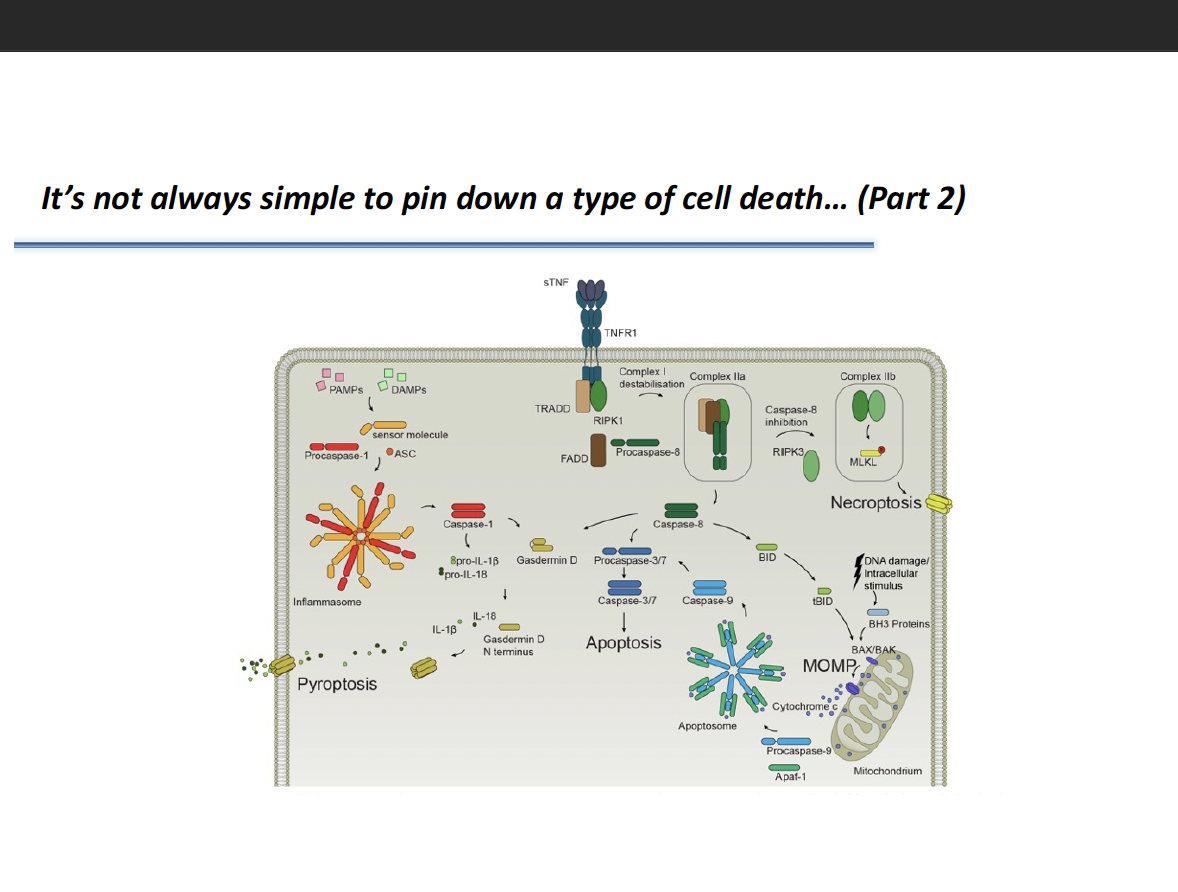
\includegraphics[width=1\textwidth]{Images/CellDeath.png}\\[1cm]

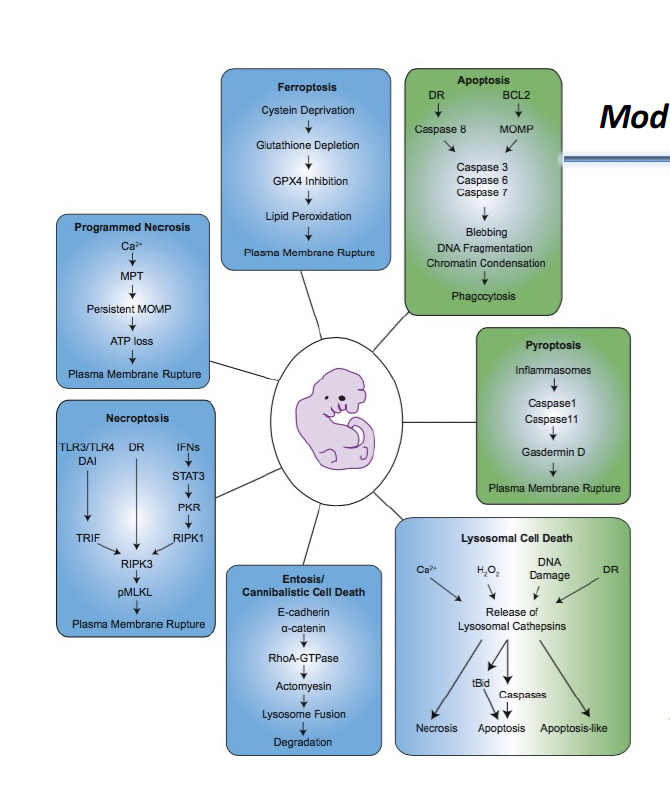
\includegraphics[width=1\textwidth]{Images/Types.png}\\[1cm]


\subsubsection{Elimination of damaged or infected cells}
\begin{itemize}
    \item Elimination of infected cells or transformed cells by apoptosis: Cytotoxic cells can kill virus infected cells or tumour cells and cause apoptosis.
    \item Elimination of infected cells by necrosis: Cells infected with a virus or bacteria cause necroptosis or pyroptosis which cause the cell to burst, releasing DAMPs and pro-inflammatory cytokines, leading to inflammation.
\end{itemize}

\subsubsection{Sensing danger: PAMPs and DAMPs}
PAMPs: Pathogen associated molecular pattern
\\DAMPs: DAMPs, or danger-associated molecular patterns, are molecules that are released by cells during injury or stress and are recognized by the immune system as signals of tissue damage. They can be considered as "danger signals" that alert the immune system to the presence of cellular damage or stress and trigger an inflammatory response.

\subsubsection{PAMPs are recognized by different receptors}
unique to pathogens and are recognized by the host's immune system as signals of an infection. They differ from DAMPs, which are molecules that are released by host cells and are recognized by the immune system as signals of tissue damage.

PAMPs are recognized by a different set of receptors on the host's immune cells called pattern recognition receptors (PRRs). Examples of PRRs include:

Toll-like receptors (TLRs): TLRs are receptors that are found on the surface of immune cells and are capable of recognizing a wide range of PAMPs, including lipopolysaccharides (LPS) from gram-negative bacteria, and viral double-stranded RNA.
NOD-like receptors (NLRs): NLRs are receptors that are found in the cytoplasm of immune cells and are capable of recognizing PAMPs from both bacteria and viruses.
RIG-I-like receptors (RLRs): RLRs are receptors that recognize viral RNA and are found in the cytoplasm of immune cells
C-type lectin receptors (CLRs): CLRs are receptors that recognize carbohydrates and are found on the surface of immune cells.
PPRs: PPRs are receptors that recognize nucleic acids, such as viral DNA and RNA.
\subsubsection{DAMPs are recognized by different receptors}
TLR2 and TLR4: MGB1, HSP, histone, hyaluronic acid, biglycan
\\TLR3, TLR7, TLR9: Self-nucleic acids
Other receptors include:
\\NOD-like receptors (NLRs) : These receptors are located in the cytoplasm of cells and can recognize a variety of DAMPs, including ATP and HMGB1.
\\RIG-I-like receptors (RLRs) : These receptors are also located in the cytoplasm of cells and can recognize viral RNA and other DAMPs.
\\C-type lectin receptors (CLRs) : These receptors are found on the surface of cells and can recognize carbohydrates and other DAMPs.
\\Toll-like receptors (TLRs) : These receptors are also found on the surface of cells and can recognize a variety of PAMPs and DAMPs.
\subsubsection{Cell death proteins modulating inflammation and the immune response?}
\begin{itemize}
    \item 
\end{itemize}
\subsubsection{Inflammatory mediators}
\begin{itemize}
    \item Tumor necrosis factor (TNF)
    \item IL-1 family members
    \item IL-6
    \item Interferon (IFN)
    \item iNOS/ROS
    \item Prostaglandins
\end{itemize}

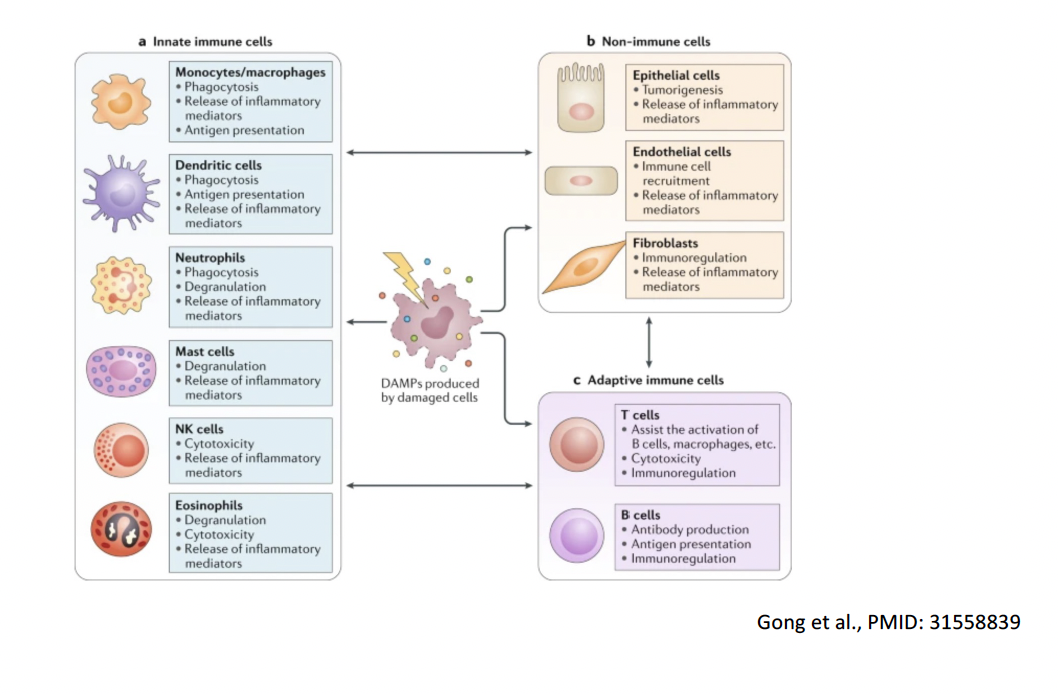
\includegraphics[width= 1\textwidth]{Images/Immunity.png}\\[1cm]
\subsubsection{Neurological disease: loss of neurons in specific locations in the brain}
In Alzheimer's Disease, there is atrophy of the hippocampus, the ventricles were enlarged, and the cerebral cortex show evidence of atrophy as well. In addition, there is a loss of dopaminergic neurons in te substantia nigra.


\subsubsection{Summary of the Whole Lecture}
Apoptosis, pyroptosis, and necroptosis are three different types of cell death that occur in cells.

Apoptosis is a type of programmed cell death that is controlled by the cell itself. It is triggered by a variety of internal and external signals, such as DNA damage, growth factor deprivation, and viral infections. Apoptosis is characterized by the activation of caspases, a family of proteases that cleave and degrade specific cellular proteins. This leads to the activation of a cascade of events that result in the shrinkage of the cell, chromatin condensation, and the formation of apoptotic bodies. These bodies are then engulfed and cleared by neighboring cells or phagocytic cells, such as macrophages, without triggering an inflammatory response. Apoptosis plays a crucial role in maintaining tissue homeostasis and preventing the development of cancer.

Pyroptosis is a type of programmed cell death that is mediated by the inflammasome, a cytosolic complex that senses pathogenic and danger signals, such as bacterial and viral infections and damage-associated molecular patterns (DAMPs). The inflammasome activates caspase-1, which cleaves and activates pro-inflammatory cytokines, such as IL-1β and IL-18. This leads to the release of inflammatory mediators and the formation of a pore in the cell membrane, resulting in the death of the cell. Pyroptosis is a highly inflammatory form of cell death that plays a crucial role in host defense against pathogens.

Necroptosis is a type of programmed cell death that is mediated by the receptor-interacting protein kinase (RIPK) family of proteins. Necroptosis is triggered by a variety of signals, such as growth factor deprivation, DNA damage, and viral infections. It is characterized by the formation of large necrotic cell corpses, which are not engulfed by phagocytic cells and generate a strong inflammatory response. Necroptosis is thought to play a role in host defense against pathogens and the elimination of cancer cells.

All three types of cell death are activated by different signaling pathways, however, they all play a crucial role in maintaining tissue homeostasis, preventing the development of cancer, and defending against pathogens.

PAMPs (Pathogen-associated molecular patterns) are molecules that are unique to pathogens and are recognized by host cells to initiate an innate immune response. These molecules are involved in the detection of pathogens by activating the inflammasome and triggering pyroptosis.

DAMPs (Damage-associated molecular patterns) are molecules that are released from stressed or damaged host cells and are recognized by the host cells to initiate an innate immune response. These molecules are involved in the detection of cell damage by activating the inflammasome and triggering pyroptosis.

\section{Microglia}
Brain Cells
\begin{itemize}
    \item Neurons
    \itemize Non-neuronal cells: GLIA
    \begin{itemize}
        \item Oligodendrocyte
        \item Astrocyte
        \item Microglia: the resident macrophahges in te brain (5-12$\%$ of brain cells)
    \end{itemize}
\end{itemize}

\subsubsection{Macrophages}
Macrophages:
\begin{itemize}
    \item Are phagocytic
    \item Repair tissues after inflammation
    \item Clear foreign and senescent cells
    \item Play a role in innate immunity
    \item Are important to tissue homeostasis
\end{itemize}

\subsubsection{What is Phagocytosis?}
\begin{enumerate}
    \item Microbe binds to phagocyte receptors
    \item Phagocyte membrane zips up around the microbe
    \item Microbe is ingested in phagosome
    \item Fusion of phagosome with lysosome
    \item Killing of microbes by ROS, NO, and lysosomal enzymes in phagolysosomes
\end{enumerate}

\subsubsection{Antibody-mediated opsonization}
\begin{enumerate}
    \item Opsonization of microbe by IgGG
    \item Binding of opsonized microbes to phagocyte Fo receptors
    \item Fo receptor signals activate phagocyte
    \item Phagocytosis of microbe
    \item Killing of ingested microbe
\end{enumerate}


\subsubsection{Macrophage Activation}
\begin{enumerate}
    \item Activation of macrophages
\item Responses of activated macrophages
\begin{itemize}
    \item Enhanced killing of phagocytosed bacteria
    \item Secretion of inflammatory cytokines
    \item Increased expression of molecules required for T cell activation
\end{itemize}
\end{enumerate}

\subsubsection{Tissue Resident Macropages}
\begin{itemize}
    \item Macropaghages are present in each tissue
    \item Macrophages have different roles in each tissue
    \item Macrophages contribute to tissue homeostasis ('Housekeeping roles')
    \item Macrophages are imprinted by the tissue environment
\end{itemize}
\subsubsection{Microglia-The Resident Macrophages in the CNS Parenchyma}
Microglia:
\begin{itemize}
    \item Innate sentinels, "te first line of defense" in the CNS
    \item Dendritic morpology
    \item "Grid-like" distribution
    \item Constantly retracting and extending their processes
    \item Highly dynamic
    \item Scanning their environment
\end{itemize}

\subsubsection{Microglia Signature Genes}
Microglia have unique microglia signature. 
\\Microglia also have conserved core gene program across evolution. Spi1, irf8, Sall1, Gm, Cst3, Mertk, P2ry12, Trem2, exb Apbb1ip, Mef2a, Bin1, cd81, Tardbp

\subsubsection{Hematopoiesis}
Bone Marrow: The site of ematopiesis: 
\begin{enumerate}
    \item Hematopoietic stem cell
    \item Monocyte/dendritic cell precursor
    \item Monoblast
    \item Monocyte
    \item Macrophage
    \item Activated macrophages
\end{enumerate}
\subsection{Bone Marrow Transplantation}
\begin{enumerate}
    \item Total Body Iradiation
    \item Donor Hematopoietic stem cells (HSCs)
    \item Microglia are Not replaced by BM-derived cells
    \item Immune cells (including monocytes) are replaced by new donor cells
\end{enumerate}
\subsubsection{Developmental Hematopoiesis}
Initially, primitive hematopoiesis takes place in the Yolk sac in the mother's womb. Then, definitive hematopoiesis takes place in the fetal liver and after birth it takes place in the bone marrow.

\subsubsection{Yolk Sac Macrophages Give Rise to Microglia}
Runx1$^{CreER}$YFP$^{LSL}$ were injected to yolk sac macrophages. Later, when microglia were analyzed, it was demonstrated that microglia self-maintain locally without circulating monocytes and that they were derived from Yolk Sac Macrophages.
\\Early erythromyeloid precursors (EMPs) in the
yolk sac differentiate into primitive
macrophages, which colonize the developing
brain and give rise to the adult population of
microglia.
\\Microglia self-maintain locally without the input
of circulating monocyte

\subsubsection{Does Ontogeny Matter?}
Exchange of resident microglia with 'monocyte-derived' microglia
\begin{enumerate}
      \item In the experiment, we have a microglia-deficient brain
      \item Donor cells engraft in a microglia-deficient
brain
      \item Microglia-like cell repopulation
\end{enumerate}
In this experiment, it was shown that added mononcytes in the brain had a different signature compared to embryonically-derived microglia
Microglia signature genes are only expressed when they are YS-derived

\\Lineage- and tissue-specific factors imprint the microglia signature/identity,
which then translates into their tissue-specific functions

\subsubsection{Functions of Microglia in Health}
Microglia are important for neurodevelopment and brain homeostasis. Some examples include:
\begin{itemize}
    \item Microglia are important for synaptic pruning, neurogenesis, and learning-dependent synapse formation
    \item Microglia are important for wiring the forebrain
    \item Microglia regulate oligodendrogenesis and myelination
    \item Microglia regulate capillary function
\end{itemize}
\subsubsection{Microglia-Deficient Mice}
\begin{itemize}
    \item Macrophage colony stimulating factor signaling (CSF1R) is critical for the development of microglia

\item Mice lacking CSF1R lack microglia and have enlarged ventricles, OB atrophy
\item CSF1R$^{FIRE}$ mice lack microglia but do not have neurodevelopmental abnormalities
\end{itemize}

\subsubsection{"Reactive" Microglia}
TGF-b Signaling is important for microglia
development, maturation and their
quiescence. Loss of TGFBR signaling in microglia leads to reactive and dysmature microglia and the development of motor neuron deficits.
\subsubsection{Disease-Associated Microglia (DAMs)}
Disease-associated microglia (DAM) are a subtype of microglia, which are the resident immune cells of the central nervous system (CNS). In a healthy brain, microglia play important roles in maintaining the proper functioning of the CNS, including supporting neuron survival, synapse formation and pruning, and clearing away cellular debris. However, in certain neurological and neurodegenerative diseases, such as Alzheimer's disease, multiple sclerosis, and Parkinson's disease, microglia can become activated and take on a "disease-associated" phenotype. These DAM are characterized by changes in their gene expression, morphology, and function, and are thought to contribute to the pathology of these diseases.

\\Senescent microglia in ageing show similar profile as DAMs in AD
\\Aged microglia show:
\begin{itemize}
    \item Functional impairments:
    \begin{itemize}
        \item Reduced engulfment of amyloid-$\beta$
        \item reduced process mobility, chemotaxis, and migration
        \item increased activation and enhanced release of inflammatory cytokines
        \item loss of neuroprotective potential
    \end{itemize}
\end{itemize}
\\AD microglia show:

    \begin{itemize}
        \item reduced and ineffective A$\beta$ phagocytosis and digestion
        \item C3 receptor-mediated microglia activation
        \item microglia depletion does not affect plaque formation and neurodegeneration
    \end{itemize}
We believe that APP (Ampyloid$\beta$ plaque) formation and $\alpa$Syn aggregates/Lewy body formation leads to te Aged microglia $\rightarrow$ Neurodegenerative microglia transition.

\subsubsection{Microglia Heterogeneity, Diversity, and States}
Microglia spatial diversity and states:
\begin{itemize}
    \item Density
    \item Morphology
    \item Signature
    \item Sex-Difference
    \item Clearance/pruning
    \item Metabolism
\end{itemize}
\\In the old view: there was the idea of dichotomy in microglia: Good vs Bad
\begin{itemize}
    \item Good Microglia
    \begin{itemize}
        \item Resting
        \item Ramified
        \item M2
        \item Anti-inflammatory
    \end{itemize}
    \item Bad Microglia
    \begin{itemize}
        \item Activated
        \item Ameboid
        \item M1
        \item Pro-inflammatory
    \end{itemize}
    
\end{itemize}
Now, the new view is that there are different states of Microglia, such as:Epigenetic, proteonic, metabolomic, transcriptomic.
\\Tan et al 2020:
\\Abstract
\\Microglia have been recently shown to manifest a very interesting phenotypical heterogeneity across different regions in the mammalian central nervous system (CNS). However, the underlying mechanism and functional meaning of this phenomenon are currently unclear. Baseline diversities of adult microglia in their cell number, cellular and subcellular structures, molecular signature as well as relevant functions have been discovered. But recent transcriptomic studies using bulk RNAseq and single-cell RNAseq have produced conflicting results on region-specific signatures of microglia. It is highly speculative whether such spatial heterogeneity contributes to varying sensitivities of individual microglia to the same physiological and pathological signals in different CNS regions, and hence underlie their functional relevance for CNS disease development. This review aims to thoroughly summarize up-to-date knowledge on this specific topic and provide some insights on the potential underlying mechanisms, starting from microgliogenesis. Understanding regional heterogeneity of microglia in the context of their diverse neighboring neurons and other glia may provide an important clue for future development of innovative therapies for neuropsychiatric disorders.




\subsubsection{The CNS: An Immune Privileged Site}
The CNS Borders are:
\begin{itemize}
    \item The meninges
    \begin{itemize}
        \item Dura mater 
        \item arachnoid mater
        \item pia mater
    
    \end{itemize}
    \item Choroid plexus
    \item Perivascular spaces
\end{itemize}

Original concept of an immune privileged site:
\begin{itemize}
    \item  Implanted tissue grafts do not elicit
immunity leading to graft rejection
\item Evasion of immune recognition
\item Absence of lymphatic vessels
\item Presence of a blood-brain barrier (BBB)
\end{itemize}

Revised:
\begin{itemize}
    \item  Grafts are rejected when transplanted
into the ventricles
\item CSF drains to deep cervical lymph
nodes
\item Lymphatic vessels in the dura
\item T cells cross the BBB in the absence of
inflammation
\end{itemize}

\subsubsection{CS Macrophages: Microglia and BAMs}
Microglia and BAMs are different.


\subsubsection{Immune Cells Diversity at the CNS Borders}
Mass cytometry of CNS including the borders show that microglia are the largest immune cell population, with the second place being BAMs. Other immune cells exists as well, albeit in smaller amounts.

\subsubsection{The Dural Sinus Hub}
The dural sinuses are a group of large venous channels that drain blood from the brain and skull. They are located in the dura mater, which is the outermost layer of the meninges that surrounds the brain and spinal cord. The dural sinus hub is a term used to describe the area where several dural sinuses converge and drain into larger veins.

\\Recent studies have shown that the dural sinus hub is an important site of immune surveillance within the brain. It has been found that the dural sinus hub is rich in immune cells, including macrophages and T cells, which are able to migrate to the brain and spinal cord and participate in immune responses. These immune cells are thought to be involved in the surveillance of the brain and skull, and are able to detect and respond to pathogens and other foreign invaders that may enter the brain through the dural sinuses.

\\The dural sinus hub also contains specialized cells called "pericytes" that are able to control the permeability of the blood-brain barrier and regulate the exchange of blood and cerebrospinal fluid between the brain and the blood vessels.
\subsubsection{Immune Surveillance and Meningeal Immunity}
T cells
\begin{itemize}
    \item T cell signals are important for brain homeostasis and function of the brain
\item Mice lacking T cells have an impaired ability to perform spatial learning, memory tasks and also have social deficits, anxiety-like and depression-like behaviors (reviewed in de Lima et al. 2020, Ma et al. 2021)
\item Development of PML induced by the JC virus in immunocompromised hosts
\end{itemize}

Macrophages (BAMs)
\begin{itemize}
    \item  Perivascular macrophages: Integrity of the BBB, vasoconstriction
\item Hydrocephalus observed in mice lacking macrophages including choroid plexus
macrophages: role in CSF homeostasis? (reviewed in Munro et al. 2022).
\end{itemize}

\subsubsection{Immune Surveillance}
There needs to be a balance between tolerance and immunity. If there is too much immunity, there can be autoimmunity. If there is too much tolerance, this can lead to tumor development. 

\\Tolerance
\begin{itemize}
    \item Ag-specific tolerance (MHCII) 
    \item inhibitory checkpoint molecules
    \item Immune suppressive factors (TGF-b, IL-10)
\end{itemize}
\\Immunity
\begin{itemize}
    \item Ag-specific T cell activation
    \item Co-stimulation
    \item proinflammatory cytokines
\end{itemize}
\subsubsection{Homeostatic Functions of Immune Cells in the Brain}
Tissue support: by BAMs and Microglia
\\Immune surveillance: by patrolling immune cells

\section{}{Autoimmune Disorders (Myasthenia gravis, Neuromyelitis optica, MS)}

\subsection{Learning Objectives}
Objective 1: Describe the pathogenesis, clinical manifestations
and treatment options for Myasthenia gravis
 = prototypical antibody mediated neurological disorder
\\ Objective 2: Get to know typical findings of Neuromyelitis optica
spectrum diseases, relevance of AQP4-antibodies

\subsubsection{Pathomechanism at the Neuromuscular Endplate}
The NMJ is vulnerable to toxins, autoantibodies, genetic abnormalities
\begin{itemize}
    \item 1975: Appel et al.: Detection of
AChR-reactive antibodies in
MG patients
\item 2001: Vincent et al.: MuSKreactive
antibodies
\item 2011-2012: Higuchi, Peyzner,
Zhang et al.: LRP4-reactive antibodies
\end{itemize}

\subsubsection{Immunopathology}
Localization of IgG at a neuromuscular junction in Myasthenia Gravis
\\Antibodies bind to the AChR (80-85%)
\begin{itemize}
    \item – Complement-mediated destruction
\item Accelerated internalization and degradation
\item Blocked ACh-AChR binding
\item Anti-MuSK (10$\%$): IgG4, do not fix complement, adversely affect AChR clustering
\end{itemize}

\subsubsection{Autoimmune Myasthenia gravis}
 The thymus is abnormal in most patients
 \begin{itemize}
     \item - Lymphoid follicular hyperplasia or thymoma
\item AChR epitope expression on myoid cells/ thymoma
likely involved in initiation of the anti-AChR immune
response
 \end{itemize}
 Genetic predisposition
 \begin{itemize}
     \item Monocygotic twins: 30-40$\%$ concordance rate
\item GWAS: Certain HLA types predispose to MG
\item Other associated autoimmune disorders

 \end{itemize}

 May begin at any age, early peak: 20-30, ♀ $>$ ♂
late peak (increasing): 60-80,
\subsubsection{Myasthenia Gravis: Disease Course}
About 80$\%$ present with eye symptoms: Double vision or eye droop
\\Only 15$\%$ remain ocular at 3 years

\\Risk factors for generalization:
\begin{itemize}
    \item female, seropositivity (MuSK $>$ AChR
    \item Unclear, if immune terapy reduces risk of generalization, conflicting retrospective data. No randomized contol data
\end{itemize}

\\MG Mortality: Prior to 1960: 30$\$$, now less than 1$\%$ die. This is due to mechanical ventilation, prednisone...
\\Most patients improve and go into remission

\subsubsection{MG Clinical Presentation}
Case 1: " I cannot chew my steak"
\\54 years old man
Was unable to chew without
supporting his chin with his
hand = jaw ptosis
Not painful, like in jaw
claudication = inability to
chew because of pain
(temporal arteritis)
After treatment with plasmaperesis he was better.
\subsubsection{MG: Diagnostic Tests}
\begin{itemize}
    \item Edrophonium Test (Tensilon)
\begin{itemize}
    \item inhibits ACh degradation: $\uparrow$ACh)
\end{itemize} 
\item Autoantibodies
\begin{itemize}
    \item anti-AChR, less common: anti-MuSK, -LRP4)
\end{itemize}
\item Electrophysiology:
Repetitive nerve stimulation, single-fiber EMG
\item Other Tests:
\begin{itemize}
    \item Thyroid
\item TPMT activity
\item chest CT or MRI
\end{itemize}

\end{itemize}

\subsubsection{MGyastenia Gravis: Therapy}
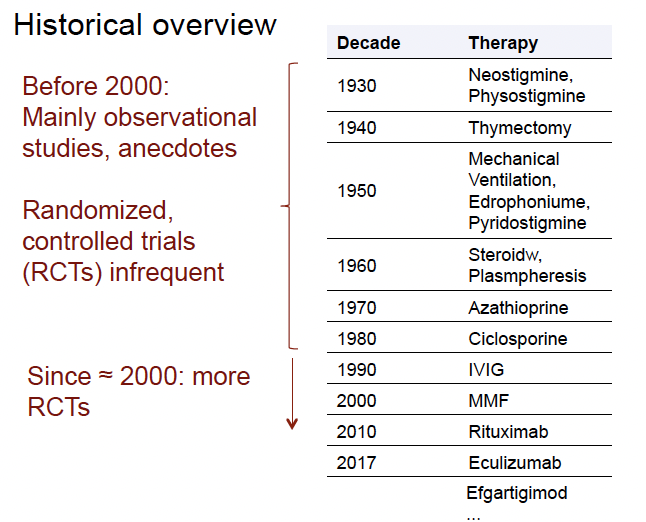
\includegraphics[width=1\textwidth]{Images/MGThera.png}\\[1cm]

Acetylcholinesterase Inhibitors:
\begin{itemize}
    \item Since 1930s: symptomatic
treatment of choice for MG
\item Inhibit the breakdown of
acetylcholine at the
neuromuscular junction
\item Increased signalling
\item Relieve of symptoms
\item Pyridostigmin was granted FDA
approval in 1955 as oral tablet.
\end{itemize}

\subsubsection{Myasthenia Gravis: Therapy (Continued)}
\\Steroids: work well, but have long-term side
effects
\\Immunosuppressants:
\begin{itemize}
    \item Azathioprine
\item Mycophenolate Mofetil (safe contraception)
\item Intensified therapy: rituximab (in particular
MuSK myasthenia)
\end{itemize}

Problems: Still little robust RCT data, delayed onset of action
\\
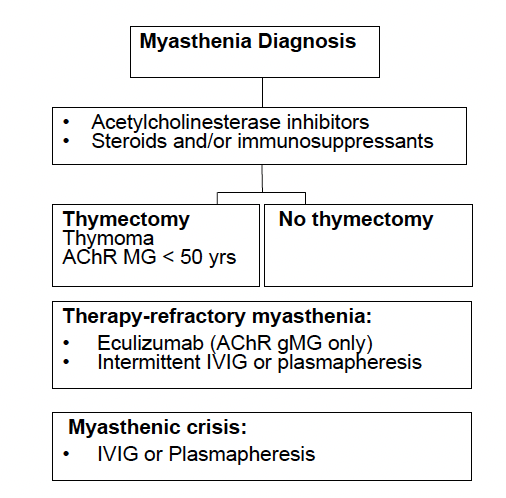
\includegraphics[width=1\textwidth]{Images/MGD.png}\\[1cm]



\subsubsection{New Therapy}
New monoclonal antibodies
\begin{itemize}
    \item B-cell and plasma cells-directed antibodies
    \item Complement inhibitors
    \item Neonatal FC receptor inhibitors
\end{itemize}
Monoclonal antibodies (mAbs) are a type of therapy that target specific molecules or cells in the body. In the case of MG, several monoclonal antibodies have been developed to target the acetylcholine receptors, or the antibodies that attack them. These mAbs have been shown to be effective in improving muscle strength and function in patients with MG.

\\One example of a monoclonal antibody used to treat MG is eculizumab. Eculizumab is a humanized monoclonal antibody that targets the complement protein C5, which is involved in the formation of the immune complex that attack acetylcholine receptors. By inhibiting C5, eculizumab reduces the formation of these immune complexes, thereby reducing the destruction of acetylcholine receptors, and improving muscle strength in patients with MG.

\\Another example of a monoclonal antibody used to treat MG is rituximab, it works by targeting a protein called CD20 which is present on the surface of B cells, a type of immune cell that produces the antibodies that attack the acetylcholine receptors. By targeting and depleting these B cells, rituximab reduces the production of these harmful antibodies, improving muscle strength and function in patients with MG.
\subsubsection{Neuromyelitis optica spectrum disorders}
Neuromyelitis optica - Inflammatory disorder of the CNS characterized by
recurrent attacks of optic neuritis and transverse myelitis
Aquaporin-4 IgG is a serum biomarker found in 80$\%$ of patients
\begin{itemize}
    \item • Specific biomarker of neuromyelitis optica
\item allowed distinction from MS
\item Led to recognition of a wider spectrum of clinical manifestations,
including brainstem, diencephalic and cerebral syndromes,
resulting in the current term:
“neuromyelitis optica spectrum disorders”
\end{itemize}

\subsubsection{NO Spectrum Disorders History}
\begin{enumerate}
    \item Devic Syndrome
    \item NMO: Variant of MS? 
    \item Anti-Aquaporin-4 Antibodies
    \item “… Contemporary diagnostic criteria require
absence of clinical disease outside the optic
nerve or spinal cord.
We have, however, frequently encountered patients
with a well-established diagnosis of NMO in whom
either asymptomatic or symptomatic brain
lesions develop suggesting that the diagnostic
criteria for NMO should be revised.”
\end{enumerate}

\subsubsection{NMOSD-IPND Criteria 2015}
\\• Increased specificity versus MS
\\• Increased sensitivity compared to 2006 criteria
\\• Broader spectrum of clinical and MRI findings
\\• Facilitate earlier and more accurate diagnosis
\\• AQP4-IgG seropositive diagnosis with 1 attack
\\• Earlier initiation of treatment
\\• Epidemiologic studies
\\• Clinical trials

\subsubsection{Criteria for AQP4-IgG+ NMOSD}
1. At least one core clinical characteristic
\begin{itemize}
    \item A. Optic neuritis
\item B. Acute myelitis
\item C. Area postrema syndrome: hiccups, nausea, vomiting
\item D. Acute brainstem syndrome
\item E. Symptomatic narcolepsy or acute diencephalic clinical syndrome with NMOSD-typical
diencephalic MRI lesions
\item F. Symptomatic cerebral syndrome with NMOSD-typical brain lesions
\end{itemize}

2. AQP4-IgG+ (cell-based assay)
\\3. Exclusion of alternative diagnoses
\subsubsection{Aquaporin-4 IgG}
• Discovered in patients with neuromyelitis optica in 2004
\\• AQP4 is the most common water channel in the CNS, expressed in the astrocyte endfeet
\\• APQ4+NMOSD is considered an autoimmune astrocytopathy
\\• AQP4-IgG is pathogenic
Pathology:
\begin{itemize}
    \item Inflammatory infiltrates,
\item axonal loss & demyelination
\item  Perivascular deposition of
\begin{itemize}
    \item immunoglobulins and
\item complement
\end{itemize}

\item Loss of AQP4 in astrocytes
\end{itemize}
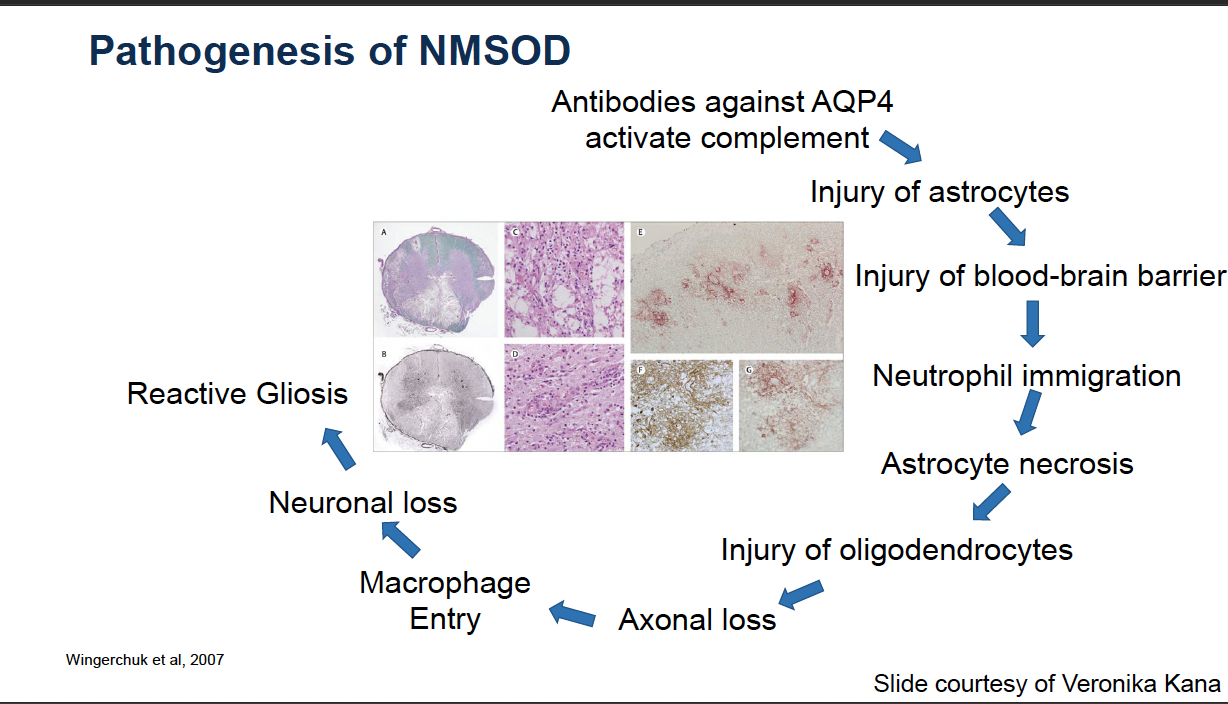
\includegraphics[width=1\textwidth]{Images/PathogenesisNMSOD.png}\\[1cm]
\subsubsection{Epidemiology AQP4+ NMOSD}
Prevalence varies between populations and
geographic location.
\\Higher prevalence in non-white populations:
\begin{itemize}
    \item Afro-Caribbeans, African-Americans
~ 1/10,000
\item Whites ~ 1/25,000
\end{itemize}
• More common in females (9:1)
• Onset fourth decade
\begin{itemize}
    \item 5$\%$ cases pediatric
\item 12$\%$ cases $>$65 years
\end{itemize}

\subsubsection{AQP4+ NMOSD - Clinical Manifestations}
Spectrum of clinical manifestations
\begin{itemize}
    \item  Optic neuritis
\item Transverse myelitis
\item Area postrema syndrome, and other brainstem
\item Diencephalic syndrome
\item Cerebral syndrome
\end{itemize}

\\• Severe attacks, which can result in permanent deficits
\\• Relapsing course, no secondary progression
\\• Frequent coexisting autoimmunity
(SLE, Sjogren, antiphospholipid Ab)

\subsubsection{NMSOD Diagnostics}
NMSOD Diagnostic tests
comprehensive history and examination
\begin{itemize}
    \item Core clinical features, exclude DDs
\end{itemize}
brain and spinal cord neuroimaging with MRI
\\determination of AQP4-IgG antibody status
\begin{itemize}
    \item Serum more sensitive than CSF
\item Cell-based assays: higher specifity and sensitivity, FACS
\end{itemize}
Lumbar puncture+CSF analysis
\begin{itemize}
    \item - 50$\%$ pleocytosis, WBC $>$ 100 in 6$\%$ cases.
\item Neutrophils, eosinophils, may be present.
\item CSF-unique OCB in $<$20$\%$.
\item GFAP levels elevated during attacks
\end{itemize}

\subsubsection{NMSOD: Treatment}
ACUTE ATTACKS
\begin{itemize}
    \item  Glucocorticoid therapy: iv methylprednisolone (1g/d for 3-5 days)
Severe symptoms or vision loss, poorly responsive to steroids:
\item Plasma exchange
\end{itemize}
 ATTACK PREVENTION
immunotherapy, to reduce the risk of relapse as soon as the
diagnosis of NMOSD is made.
\\with AQP4-IgG: Eculizumab (≈94$\%$ risk of relapse reduction), satralizumab
(≈75$\%$) or off-label: inebilizumab (≈77$\%$; US, Japan, not yet approved in CH),
rituximab or tocilizumab, others (AZP, MMF, aHSCT)
› without AQP4-IgG: all off-label

\subsubsection{Targets for approved NMOSD immunoterapies}
Rituximab: anti-DC20
\\Inebilizumab: anti-CD19
\\Satralizumab: anti-IL-y
\\Eculizumab: anti-C5

\subsubsection{NMOSD Multidisciplinary Team}
\\• Neurologist, Nurse specialist
\\• Pain Specialist
\\• Ophthalmologist
\\• Urologist
\\• Psychologist
\\• Occupational therapist
\\• Physiotherapist
\\• Dietician

\subsubsection{AQP4 vs MS}
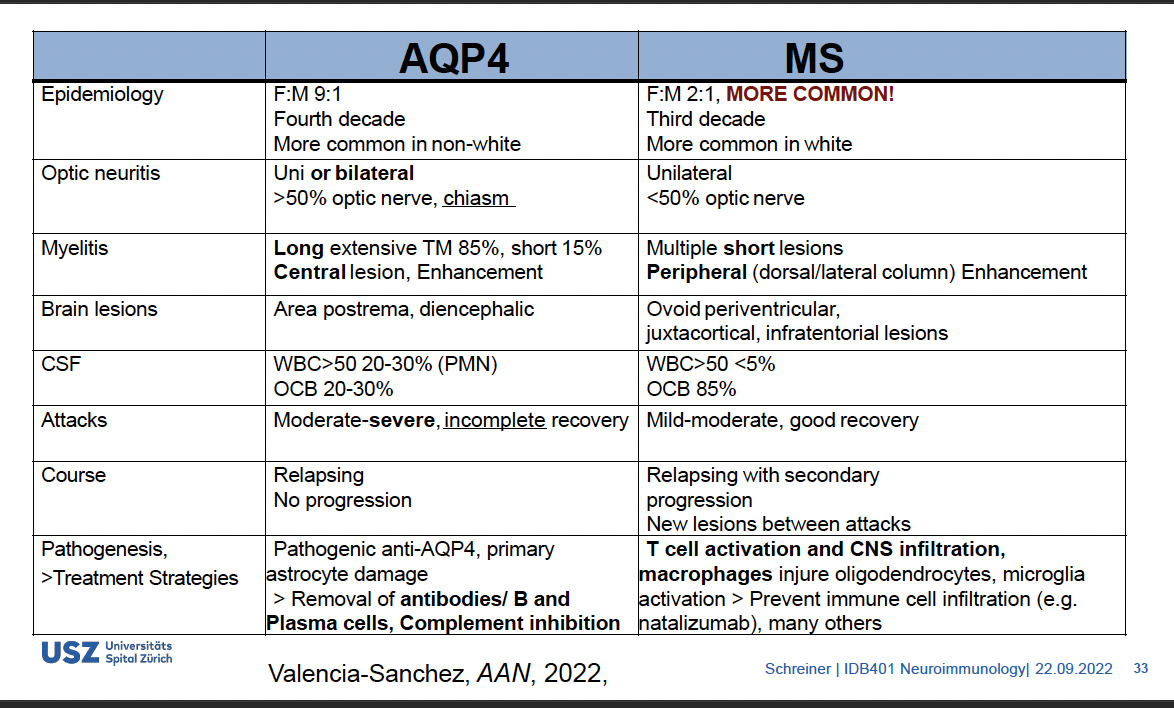
\includegraphics[width=1\textwidth]{Images/AQP4 vs MS.png}\\[1cm]

\section{Multimodal Census of Neuronal Cell Types}

\section{Multimodal census of neuronal cell types}

\subsubsection{Synapses, neurons, circuits}
Cell types are very important to understand.

\subsubsection{Diversity of neuronal cell type}

\subsubsection{Data modalities for neuronal classification}
Some different modalities to do so:
\begin{itemize}
    \item Neuronal morphology
    \item Biophysical properties, action potential firing
    \item In vivo activity (for different types of behavior)
    \item Neurochemical and synaptic markers
    \item Gene expression profiles
\end{itemize}
Brain atlases:
\begin{itemize}
    \item paper
    \item BRAIN (Huge research with lots of money going into brain atlases and BRAIN.
\end{itemize}

\subsubsection{Neuronal morphology I (neuroanatomy)}
This slide concerns cells in the hippocampus
\\There are two main classes of dendrites (in horizontal and vertical directions)
\\In the picture on the slide, the colored ones are axons, the black ones are dendrites.
\\Axons vary in cell layer distribution
\\Red: form synapsis on axon of cell
\\Example: basket cells are light blue

\subsubsection{Neuronal morphology II (neuroanatomy)}
The dendritic and axonal structures reflect possible inputs and outputs
\\Axons may form synapses on:
\begin{itemize}
    \item Dendrites (proximal or distal)
    \item Perisomatic region
    \item Axons
\end{itemize}
Axonal projections may indicate functional relevance of a cell type:
\begin{itemize}
    \item Local
    \item Long-range to specific brain regions
\end{itemize}

In Figure 4, there are two basket cells that project into cell layers. 

\subsubsection{Biophysical properties and action potential firing (electrophysiology)}
During patch-clamp recording, depolarizing or hyperpolarizing current injections (or positive or negative voltage steps) can be used to measure:
Key biophysical parameters:
\begin{itemize}
    \item  Input resistance
\item Capacitance
\item Resting membrane potential
\end{itemize}
Key action potential (AP) parameters:
\begin{itemize}
\item Half-width
\item Firing threshold and frequency
\item Attenuation
\end{itemize}
Use patch pippette to record biophysical properties. Many different parameters can be read out in such experiments.
\\The patch clamp method can help identify 3 cells separately that would not work wit all cell types: RS-INT, FS-INT, CA1-PYR

\\RS-INT, FS-INT, and CA1-PYR are types of neurons in the brain. RS-INT stands for "regular-spiking interneuron," FS-INT stands for "fast-spiking interneuron," and CA1-PYR stands for "CA1 pyramidal neuron." Interneurons are nerve cells that transmit signals between other nerve cells, and pyramidal neurons are a type of nerve cell that are characterized by their triangular shape. CA1 refers to a specific area of the hippocampus, which is a region of the brain involved in memory and spatial navigation.

\subsubsection{In vivo activity (electrophysiology)}
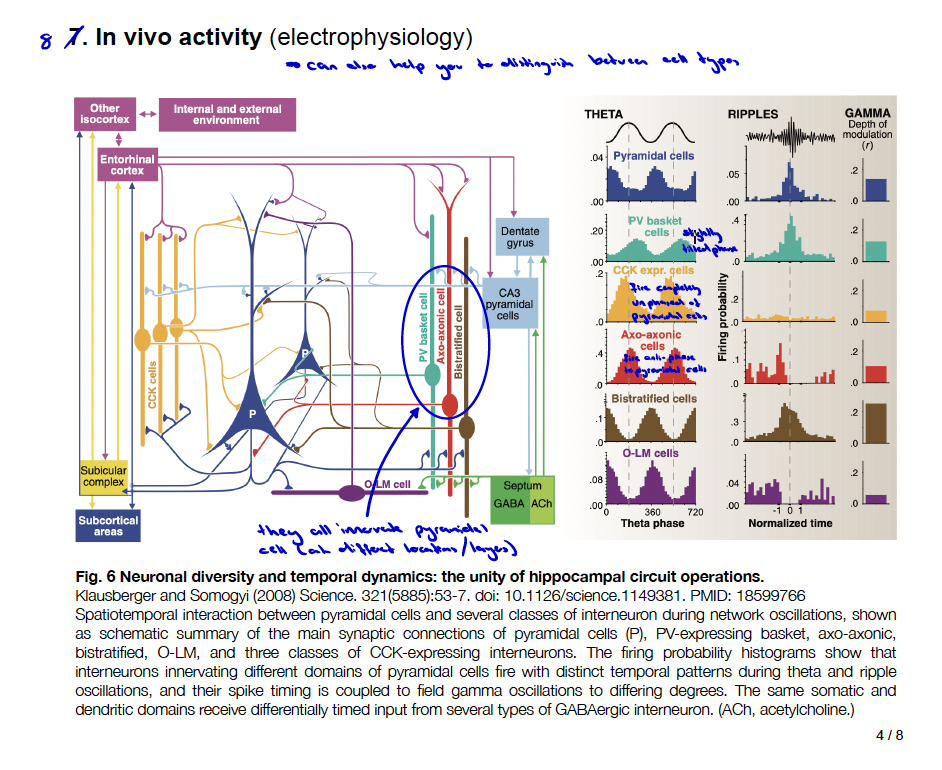
\includegraphics[width=1\textwidth]{Images/INVIVOELEC.png}\\[1cm]

\subsubsection{Neurochemical and synaptic markers (immunohistochemistry)}
Typically used markers to identify:
GABAergic interneurons (this does not identify one cell type but a specific group):
\begin{itemize}
    \item Parvalbumin (PV)
\item Cholecystokinin (CCK)
\item Somatostatin (SST)
\item Vasopressin intestinal peptide (VIP)
\item Neuropeptide Y (NPY)
\item Calbindin
\item Calretinin
\end{itemize}

Projection neurons (often sampling the biosynthesis of
neurotransmitters):
\begin{itemize}
    \item Tyrosine hydroxilase (TH) dopamine cells
\item Dopamine-b-hydroxilase (DBH) noradrenalin cells
\item Phenylethaloamine N-methyltransferase (PNMT)
adrenalin cells
\item Dopamine transporter (DAT) - dopamine cells
\item Choline acetyltransferase (ChAT) - cholinergic cells
\end{itemize}

\subsubsection{Gene Expression Profiles I (transcriptomics)}
ranscriptomic profiles identify neuronal
types. However, differences may exist
between mRNA and protein expression.
For example:
\\(1) CCK and cannabinoid type-1 (Cnr1)
immunostaining unambiguously identify CCK
neurons, but mRNA expression of the same
genes does not.
\\(2) Based on its protein expression, Camk2a
were used to generate transgenic lines to
genetically access pyramidal neurons (used
in many studies), but mRNA expression is
present in interneurons as well.
\\Distrinct mRNA and protein level are important for interpretation in Gene expession studies.
\\Cnr1: cannabinoid
\\Htr3a: neurodevelopmental marker
\\Pvalb: mostly fast spiking

\subsubsection{Gene Expression Profiles II (transcriptomics)}
Very powerful tool, we can do this for millions of cells in a single experiment.
\\Clustering of cells according to gene expression visualized on slide 11.

\subsubsection{multimodal approaches (Transcriptomics, electrophysiology, anatomy}
\begin{enumerate}
    \item Brain
    \item Electropysiology
    \item Cell Collection
    \item RNAseq
\end{enumerate}

\subsubsection{Summary and Key Points}Over the past 10-15 years, results from systems neuroscience have been making
increasingly clear that the activation of different neuronal cell types elicit specific behaviors.
\\The identification of every brain cell type is therefore not only important from a basic biological perspective but also facilitates the development of cell typespecific tools, e.g. transgenic lines.
\\However, key questions remain open…
\\Neuronal morphology, biophysical properties, in vivo activity, neurochemical and synaptic markers, and gene expression profiles (i.e. the different modalities of neuronal classification we discussed) may all reflect unique features of a cell type, but a one-to-one correspondence between the different modalities is not necessarily recognizable. 
,,They do not exist or the experiments did not have a sufficient resolution?
\\More broadly, the definition of a cell type remains debated as well as the question
if different cell types represent different entities or there is a continuous variation
between them.

\section{The CRISPR-Cas Genome Editing in the Brain}
\subsubsection{Principles of gene editing in mice}
Generation of knock-out mice
\\
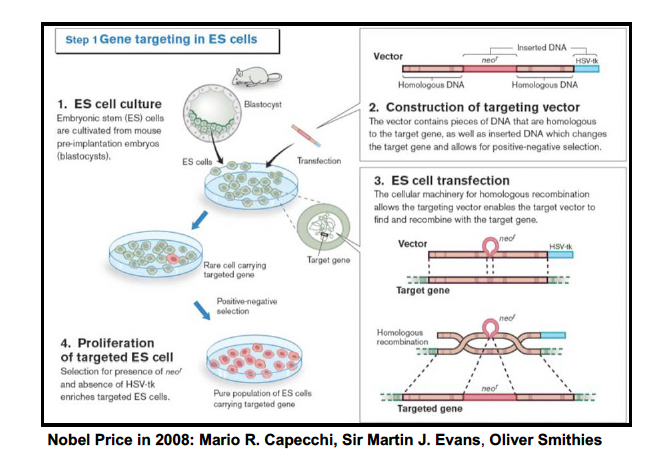
\includegraphics[width=1\textwidth]{Images/GeneEditinginMice.png}\\[1cm]
\subsubsection{Targeted nucleases: The genome editing revolution}
Zinc-finger nucleases
Zinc-finger nucleases (ZFNs) are a type of engineered endonuclease (a enzyme that cuts DNA) that are used for targeted DNA editing. They consist of a protein domain called a zinc finger, which binds to specific sequences of DNA, and the nuclease domain of the FokI endonuclease, which cuts the DNA. ZFNs allow for precise editing of the genome at specific locations, and have been used in research for applications such as gene therapy, crop improvement, and fundamental genetic research.

\\ZFNs are being replaced by newer technologies like CRISPR-Cas9 which are more versatile, efficient and cost-effective.

\subsubsection{CRISPR/Cas 9}
CRISPR - bacterial adaptive immune system.
Clustered, Regularly - Interspaced, Short, Palindromic, Repeats.
\\Repeats are 20-40 bp in length
\\Palindrome is a sequence that reads the same from left and right

\subsubsection{CRISPR Step-by-Step}
Identification of the target DNA sequence: The first step is to identify the specific DNA sequence that you want to edit. This can be done using existing genetic tools such as PCR or DNA sequencing.
\\Design of guide RNAs: Once the target sequence is identified, guide RNAs (gRNAs) are designed to specifically bind to the target sequence. gRNAs are short RNA molecules that guide the Cas9 protein to the target location in the DNA.
\\Delivery of the CRISPR-Cas9 complex: The gRNAs and Cas9 protein are delivered to the cells or organisms in which the genetic modification is to be made. This can be done by a variety of methods such as electroporation, viral vectors, or microinjection.
\\Cleavage of the DNA: The Cas9 protein uses the gRNAs as a guide to locate the target DNA sequence. Once it finds the target, it cuts the DNA, creating a double-stranded break.
\\Repair of the DNA: The cell's own repair machinery repairs the double-stranded break. If a repair template is provided, it will be incorporated into the genome at the break site. This allows for the insertion, deletion, or replacement of specific sequences in the genome.
\\Confirmation of the modification: The modified cells or organisms are screened to confirm the desired genetic modification has occurred.
\\Evaluation of the modified cells/organisms: After the modification has been confirmed, the modified cells or organisms are evaluated for the desired phenotype.

\subsubsection{Application of the CRISPR/Cas9 System}
2012: Reprogramming Cas9 to a target site by changing the sequence of the crRNA
(Siksnys and colleagues)
\\2012: Doudna, Charpentier and colleagues fused the crRNA and the tracrRNA
together to create a single, synthetic guide, and demonstrated target specific
DNA cutting in vitro
\\2013: Zhang, Church and colleagues demonstrated targeted genome cleavage in
human and mouse cells.
\subsubsection{Two Classes of CRISPR-Cas systems and their modular organization}
CRISPR-Cas systems are classified into two main classes based on their molecular architecture and functional mechanisms:

\\Class 1 CRISPR-Cas systems use a complex of multiple Cas proteins and a single, large crRNA (CRISPR RNA) molecule. The crRNA guides the Cas proteins to the target DNA and the Cas proteins cleave the target DNA. These systems are commonly used for genome editing.
\\Class 2 CRISPR-Cas systems use a single Cas protein, such as Cas9, and a small tracrRNA (trans-activating crRNA) that binds to the crRNA. The tracrRNA hybridizes with the crRNA to form a guide RNA (gRNA) that guides the Cas protein to the target DNA. These systems are also commonly used for genome editing.
Both class 1 and class 2 CRISPR-Cas systems are modular in nature, meaning that the different components of the system can be easily swapped out or replaced to target different DNA sequences.
The CRISPR array, a set of repetitive sequences, is the foundation of the CRISPR-Cas system, its transcribed into pre-crRNA and then processed into crRNA.
\\The Cas proteins, which are responsible for recognizing and cleaving the target DNA, are usually encoded by genes adjacent to the CRISPR array.
\\The crRNA or tracrRNA and Cas protein form a complex that recognizes the specific target DNA sequence and cleave it.

\\By replacing the crRNA or tracrRNA with different guide RNAs, researchers can target different DNA sequences for editing. Additionally, different Cas proteins can be used to create different types of modifications in the DNA, such as cutting, insertion, or replacement. This modularity makes CRISPR-Cas systems a powerful and flexible tool for genetic engineering.
\subsubsection{Targeted nucleases}

\subsubsection{CRISPR/Cas9 - PAM Recognition}
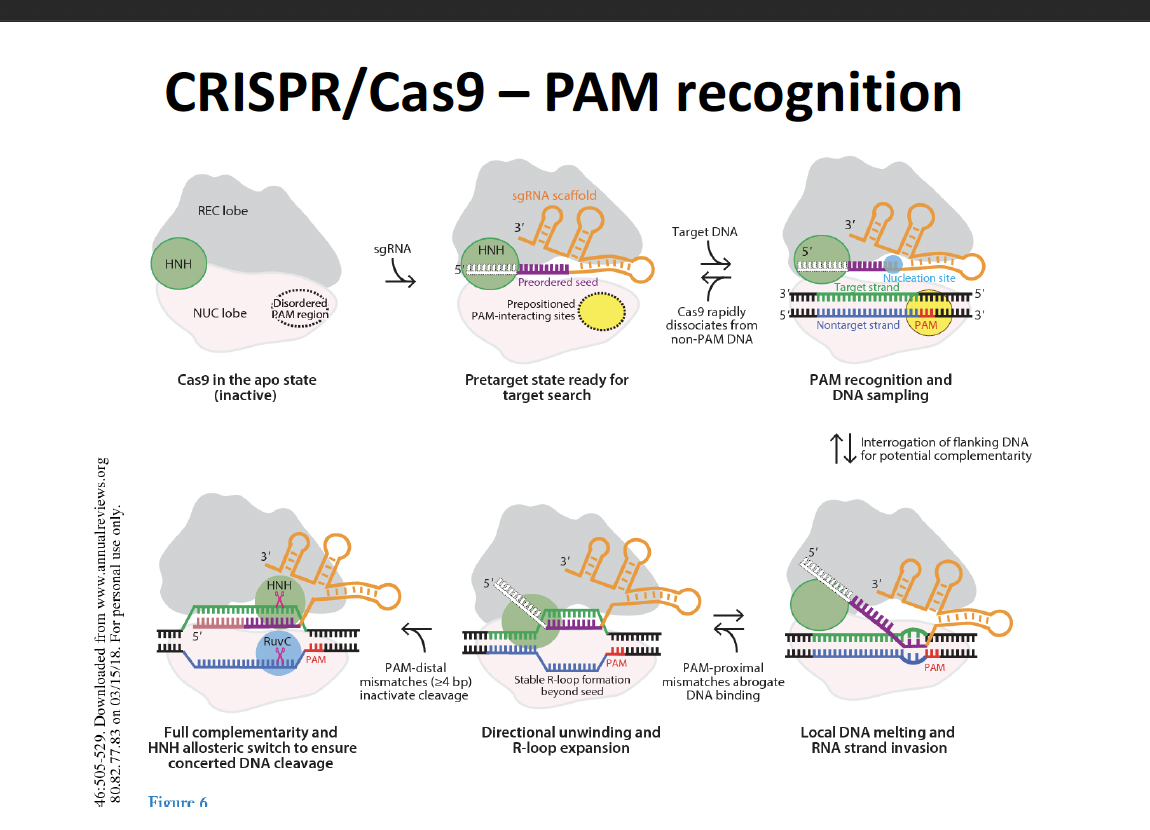
\includegraphics[width=0.8\textwidth]{Images/PAMREC.png}\\[1cm]

\subsubsection{Tools based on nuclease-impaired CRISPR-Cas systems}

    \begin{itemize}
\item Cleavage: This refers to the ability of the CRISPR-Cas system to cut DNA at specific locations. In this case, the CRISPR-Cas system has been modified so that it no longer has the ability to cut DNA, which can be useful for applications that do not require DNA cutting but still need the specificity of the CRISPR-Cas system.
\item Repression: This refers to the ability of the CRISPR-Cas system to inhibit the expression of specific genes by binding to the promoter regions of those genes. In this case, the CRISPR-Cas system has been modified so that it can no longer cut DNA, but can still bind to specific sequences and prevent the transcription of certain genes.
\item Activation: This refers to the ability of the CRISPR-Cas system to increase the expression of specific genes. In this case, the CRISPR-Cas system has been modified so that it can bind to specific sequences and enhance the transcription of certain genes.
\item Epimodification: This refers to the ability of the CRISPR-Cas system to modify the epigenetic state of a gene, which can control the expression of that gene without changing the underlying DNA sequence.
\item Imaging: This refers to the ability of the CRISPR-Cas system to be used as a tool for imaging specific sequences in the genome, either by fluorescently labeling the Cas protein or by using the Cas protein to recruit other imaging agents.
\item Nuclear reorganization: This refers to the ability of the CRISPR-Cas system to be used to change the organization of the nuclear material, such as moving a specific gene from one chromosome to another.
\end{itemize}

\subsubsection{CRISPR to Correct Genetic Diseases}
In vivo approach: CRISPR/Cas9 template; Then, either viral or non viral delivery via injection
\\Ex vivo approach: Extract stem cells, CRISPR/Cas9 correction, clonal selection, expansion.
\\OR: Fibroblast culturing, iPSC reprogramming, CRISPR/Cas9 correction, clonal selection, expansion, differentiation, and  implantation.
\subsubsection{In vivo gene therapy-delivery of genome editors to target tissues}
\begin{itemize}
    \item Viral vectors: Delivery of a DNA cassette that expresses the genome editor and sgRNA
    \item Non-viral lipid nanoparticles (LNPs): Delivery of an mRNA that encodes for the genome editor and the sgRNA.
\end{itemize}
\subsubsection{Vectors have been established from different viruses}
\begin{itemize}
    \item AAV vectors:
    \begin{itemize}
        \item Low immunogenicity
        \item Different serotypes (natural or synthetic) with tropisms for different tissues
        \item Mainly non-integrating
    \end{itemize}
\end{itemize}

\subsubsection{Diagram of rAAV transduction pathway}
Production of rAAV: The first step is to produce the rAAV vector, which is a modified version of the adeno-associated virus (AAV) that has been engineered to contain the genetic material of interest. rAAV vectors can be produced using various methods, such as plasmid transfection or viral packaging.
\\Purification of rAAV: Once the rAAV vector is produced, it must be purified to remove any impurities. This typically involves a series of centrifugation and filtration steps to separate the rAAV particles from other cellular components.
\\Delivery of rAAV to cells: The purified rAAV vector is then delivered to the target cells. This can be done by a variety of methods such as direct injection, viral transduction, or electroporation.
\\Entry of rAAV into cells: Once inside the target cells, the rAAV vector will enter the cell by binding to a specific receptor on the cell's surface. This is an essential step that enables the rAAV to be recognized by the cell, allowing it to be taken up by the cell.
\\Entry of rAAV into the nucleus: The rAAV then travels to the cell's nucleus, where the genetic material is released. The entry into the nucleus is a critical step as it allows the genetic material to be integrated into the genome and be expressed by the host cell.
\\Integration of rAAV into the genome: Once in the nucleus, the genetic material from the rAAV vector is integrated into the genome of the host cell. rAAV vectors preferentially integrate in a specific location in chromosome 19, which is relatively safe and doesn't disrupt any important gene.
\\Expression of the transgene: Once integrated into the genome, the genetic material from the rAAV vector is expressed by the host cell, resulting in the production of the protein encoded by the transgene.
\\Evaluation of the transduced cells: After transduction, the modified cells are evaluated for the desired phenotype, such as the expression of a specific protein, the correction of a genetic disease, or the modification of a specific gene.

\subsubsection{Lipid nanoparticles (LNPs) for RNA delivery}
Components of LNPs

\begin{itemize}
    \item PEG-lipid:
    \begin{itemize}
        \item They reside almost exclusively on the LNP surface, and
their concentrations control particle size
\item They create a steric barrier preventing particle
aggregation and improving in vivo circulation lifetimes.
    \end{itemize}
    \item Helper lipids (phospholipids and cholesterol)
    \begin{itemize}
        \item 
They promote formulation stability

    \end{itemize}
    \item Ionizable lipid
    \begin{itemize}
        \item  The headgroups contain tertiary amines that become
protonated under acidic pH and typically are uncharged at
neutral pH
\item The lipid tails make the molecule sufficiently hydrophobic
to promote incorporation into a nanoparticle
    \end{itemize}
\end{itemize}



\subsubsection{In vivo gene therapy in the retina}
Leber Congenital Amaurosis (LCA) is the most common cause of inherited childhood blindness, and
LCA10 is the most common form of LCA. This disease is caused by a single nucleotide mutation in
a photoreceptor gene, leading to serious vision loss or blindness within the first few months of life.
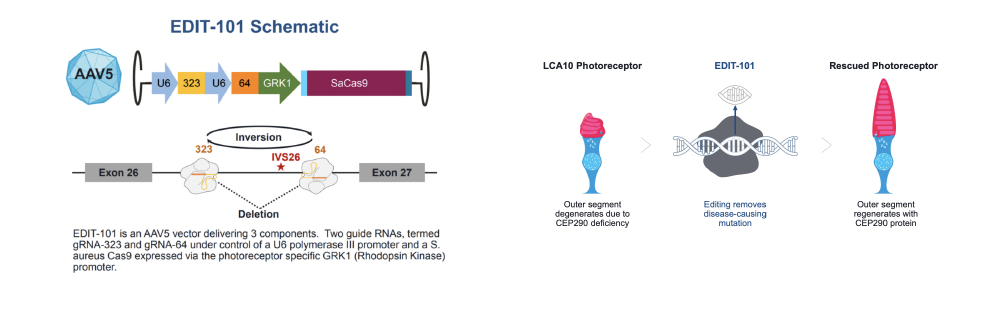
\includegraphics[width=1\textwidth]{Images/Edit101.png}\\[1cm]

\subsubsection{CRISPR to correct genetic diseases-precise editing with nucleases is inefficient in non-dividing cells}
CRISPR-mediated genome editing is a powerful tool for correcting genetic diseases by precisely editing the genome. However, the efficiency of CRISPR-mediated editing is lower in non-dividing cells compared to dividing cells.

\\Non-dividing cells, such as neurons, are less efficient at repairing double-stranded breaks in DNA than dividing cells. This is because non-dividing cells do not undergo mitosis, which is the process by which cells divide and replicate their DNA. Without mitosis, non-dividing cells are less able to repair double-stranded breaks in DNA through the process of homology-directed repair (HDR), which is the mechanism used by CRISPR-mediated genome editing.

\\Additionally, non-dividing cells have a lower level of key enzymes involved in HDR, such as DNA-dependent protein kinase (DNA-PK), which is required for the repair of double-stranded breaks.

\\Another problem is that the delivery of the CRISPR-mediated genome editing tools to the non-dividing cells is also a challenge, as these cells are often located in hard-to-reach areas, such as the brain.

\\Therefore, researchers are working on developing new methods to improve the efficiency of CRISPR-mediated genome editing in non-dividing cells, such as using different delivery methods, optimizing the repair template and alternative forms of genome editing that don't rely on HDR, like non-homologous end joining (NHEJ) or base editing.
\\NHEJ is a repair pathway that repairs double-stranded breaks in DNA without the need for a repair template, it can lead to insertions, deletions or even chromosomal rearrangements. It is less precise than HDR but it is more efficient in non-dividing cells.
\subsubsection{HDR is inefficient in the brain}
HDR (homology-directed repair) is a process by which cells repair double-stranded breaks in DNA through the use of a repair template that contains homologous sequences to the DNA surrounding the break. In the context of genome editing, this allows for the precise insertion, deletion, or replacement of specific sequences in the genome. However, HDR is less efficient in the brain compared to other tissues.

\\The main reason for this is that the brain has a low level of a key enzyme called DNA-dependent protein kinase (DNA-PK), which is involved in HDR. Without sufficient levels of DNA-PK, the cell's ability to repair double-stranded breaks through HDR is impaired. Additionally, the brain has a low rate of cell division, which also limits the efficiency of HDR.

\\Another reason is that the brain is highly complex and diverse, with different types of cells and cell populations that may have different HDR efficiencies. This makes it challenging to deliver the repair template to the right cells and achieve the desired level of precision.

\\Lastly, the brain is protected by the blood-brain barrier, which makes it harder to deliver the genetic material across the barrier and into the brain.

\\Overall, the low efficiency of HDR in the brain is a significant challenge for genome editing in the brain and researchers are trying to find ways to overcome this limitation, such as using different delivery methods and optimizing the repair template.

\subsubsection{Base editors: Cytidine deamination}
\\Base editing is a form of genome editing that allows for the direct conversion of one base to another without the need for double-stranded breaks or repair templates. This is achieved by using a specific type of enzyme called a base editor, which can make a precise change to a single base in the genome.

\\There are currently two types of base editors: cytidine base editors (CBEs) and adenine base editors (ABEs).

\\Cytidine base editors (CBEs) convert a cytosine (C) base to a thymine (T) base. This is achieved by using an enzyme called cytidine deaminase, which removes an amino group from cytosine, converting it to uracil. Then, the cell's repair machinery recognizes the uracil as a mistake and replaces it with thymine.
\\Adenine base editors (ABEs) convert an adenine (A) base to a guanine (G) base. This is achieved by using an enzyme called adenine deaminase, which removes an amino group from adenine, converting it to hypoxanthine. Then, the cell's repair machinery recognizes the hypoxanthine as a mistake and replaces it with guanine.
B\\oth cytidine deamination and adenine deamination are irreversible reactions, and the base editor can only convert one base at a time.

\\Base editing is a relatively new technology and it's still being optimized, but it has the potential to be more precise, efficient and safe compared to the traditional forms of genome editing. Base editors have already been used to correct genetic diseases in animals and are being tested in human clinical trials.
\subsubsection{Base editors: Adenine deamination}

\subsubsection{Targeting scope of base editors}
37$\%$ of pathogenic mutations are transition point mutations and theoretically targetable.

\subsubsection{Prime-editors: A highly versatile DNA double strand break-independent genome editor}
Prime editors are a new type of genome editing tool that are based on the CRISPR-Cas system. They use a modified version of the Cas9 protein and a guide RNA (gRNA) to make precise changes to the genome, but they do not rely on the creation of double-stranded breaks (DSBs) in the DNA like traditional CRISPR-mediated genome editing methods. Instead, they use a process called "prime editing" to directly convert one base to another in a specific location in the genome.

\\Prime editors consist of two main components: a prime editing guide RNA (pegRNA) and a modified Cas9 protein called prime editing Cas9 (pCas9). The pegRNA contains both the gRNA sequence that targets the specific location in the genome and a template sequence that specifies the desired change. The pCas9 protein is engineered to carry both nuclease activity, which cuts the DNA, and reverse-transcription activity, which copies the template sequence into the genome.

\\The biological mechanism behind prime editing is as follows:

\begin{itemize}
    \item The pegRNA binds to the specific location in the genome and the pCas9 protein binds to the pegRNA, creating a ribonucleoprotein complex.
\item The pCas9 protein makes a cut in the DNA at the targeted location.
\item The pCas9 protein then uses its reverse-transcription activity to copy the template sequence from the pegRNA into the DNA at the targeted location.
\item This creates a new strand of DNA that contains the desired change, and the cell's repair machinery uses this new strand to repair the cut in the DNA.
\end{itemize}



\\Prime editors are highly versatile, as they can make a wide range of changes to the genome, including point mutations, insertions, and deletions. They also have the potential to be more precise and efficient than traditional CRISPR-mediated genome editing methods, as they do not rely on the creation of DSBs in the DNA and can make changes to both coding and non-coding regions of the genome.


\section{Light-mediated discovery of surfaceome nanoscale
organization and intercellular receptor interaction networks}
\subsubsection{Surfaceome: The exposed Cell Surface
Proteome}
determines how cells can interact with the environment
\begin{itemize}
    \item cell-cell communication
    \item interaction wit pathogens
    \item binding of chemical messengers
    \item migration, adhesion, and cell survival
\end{itemize}
reflects differentiation state
\\indicates functional capacity


\subsubsection{Protein function is closely linked to the subcellular environment}
\begin{itemize}
    \item $>$50$\%$ of all proteins localize to multiple compartments
    \item only activity of subset determines function for compartment-specific processes
    \item Usually neglected in broad omics approaches
\end{itemize}

\subsection{The Surfaceome - a very social molecular interaction network}

\subsubsection{How can the surfaceome be revealed on a system-wide scale}?
\subsubsection{System-wide quantification of the cell surface proteotype and identification of extracellular glycosylation sites using autoCSC}
\begin{itemize}
    \item Tagging of cell surface residing glycoproteins with bi-functional linker probes upon gentle oxidation enables spatiotemporal surfaceome discovery
    \item AutoCSC enables quantitative surfaceome analysis with higher sensitivity, reproducibility, and throughput
\end{itemize}
Procedure is the following:
\begin{enumerate}
    \item Oxidation and biotinylation
    \item lysis and digestion
    \item High throughput processingg
    \begin{enumerate}
        \item Binding
        \item Washing
        \item Elution
    \end{enumerate}
    \item Spatial Proteotyping
    \item Cell surface N-glycopeptides with deamination at NXS/T motif
    \item DIA LC-MS/MS
    \item Identification and topology information and quantification
\end{enumerate}

\subsubsection{Cell Surface Capture (AutoCSC)tech enables system-scale analysis of the cell surface proteotype}
\begin{itemize}
    \item Cell Surface Capture enables snapshots of the
acute surface residing pool
\item Enabled applications with limited sample
amounts (> 1 Mio cells)
\item Live cell labeling - enrichment of extracellular
peptides – DIA LC-MS/MS analysis
\item Increased sensitivity and reproducibility by
automation & miniaturization
\item Phenotyping cells without antibodies
\end{itemize}
\subsubsection{Classification of Mouse B Cell Types using Surfaceome Proteotype Maps}
\\Phenotyping B cell populations without antibodies in order to identify subpopulations. Step-by-step procedure:
\begin{enumerate}
    \item Get B cells from the bone marrow, spleen, and peritoneum
    \item Flow sort into different cells via laser
    \item AutoCSC
    \item Protein cell surface expression profiles
    \item FACS validation
\end{enumerate}

\subsubsection{Dynamic regulation and nanoscale organization of the neuronal surfaceome}
\begin{itemize}
    \item Surface and intracellular protein pools
    \item Dynamic regulation of surface abundance
    \begin{itemize}
        \item Surface trafficking
        \item Protein abundance
        
    \end{itemize}
    \item Surface diffusion and synaptic targeting
\end{itemize}
\subsubsection{Unsupervised clustering reveals developmental stage specific surface expression patterns}
\begin{itemize}
    \item 6 clusters of dynamic surface protein profiles
    \item Profiles represent functional extracellular requirements
    \item Synaptic proteins largely trafficked to the surface prior synapse formation
\end{itemize}
\subsubsection{Surfaceome dynamics during neuronal development and synaptic plasticity reveal system-wide surfaceome reorganization independent of global proteostasis}
Neuronal development & synapse formation
\begin{itemize}
    \item Comprehensive time-resolved resource of the cortical culture surfaceome
\item Synaptic proteins trafficked to the surface prior synapse formation
\item Reveal wide-spread regulation on the level of surface trafficking at short time scales
\end{itemize}

Synaptic plasticity
\begin{itemize}
    \item Discovery-driven quantitative analysis of the neuronal surface during chemical LTP
\item Revealed quantitative changes beyond the AMPAR, potentially mediating the requirement of
exocytosis for LTP
\end{itemize}
Systems-scale analysis of the neuronal  surfaceome using chemoproteomic technologies

\subsubsection{Surfaceome Machine-Learning-based Predictor 'SURFY'}
Random forrest classifier on 131 features per protein and specifically per topological domain

\subsubsection{2886 Human Cell Surface Proteins}

\subsubsection{Surfaceome sizes differ across cell types}
\begin{itemize}
    \item 1,700 surfaceome genes were expressed in embryonic stem cells and derivative lines
\item The in silico surfaceome enables
\begin{itemize}
    \item the filtering of data generated by multi-omics screens and
\item supports the elucidation of the surfaceome nanoscale organization.
\end{itemize}

\end{itemize}

\subsection{How can the surfaceome interactions be revealed?}
\subsubsection{The Ligand Space}
Orphan ligand meaning: An orphan ligand is a ligand (a molecule that binds to a specific site on a larger molecule) that does not have a known receptor. This means that the ligand has been identified and its biological activity has been studied, but the specific molecule to which it binds has not yet been identified. Orphan ligands are often the subject of ongoing research in order to identify their corresponding receptors and understand their biological function.

\\Vast orphan ligand space
\begin{itemize}
    \item Engineered affinity binders
    \item Peptides, proteins
    \item secretome (sheddome)
    \item small molecules/drugs
    \item lipids
    \item viruses
    \item bacteria
    \item cells
\end{itemize}

\subsection{Finding a face in the crowd}
How do we identify cell surface targets?

How do we identify the receptors for an orphan ligand.

\subsubsection{Ligand-basd Receptor Identification Platform}
Chemoproteomic LRC (Ligand-based Receptor Capture) technology, direct identification of endogenous interactions on cells and tissues

\subsubsection{TRICEPS: Trifunctional chemoproteomic reagents allow for ligand-based receptor capture}
\begin{itemize}
    \item It’s not a pull down in the classical sense.
\item We do only label/capture pre-activated cell surface exposed N-glycosites
\item We exploit the ligand affinity to its receptor(s) to enhance chemical reaction kinetics for
labeling N-glycosites in the vicinity of the respective receptor(s.
\end{itemize}
\subsubsection{LRC has the potential to detect multiple interactions of promiscous ligands}
LRC technology does not require genetic manipulations or specific affinity binders

\subsubsection{}section{How can the surfaceome architecture be revealed on a
system-wide scale?}
Your protein does not exist. Proteoforms do.
\\Working hypothesis: Cell & proteoform-specific surfaceome sub-complexes

\subsubsection{Surfaces of T cells are not flat}

\subsubsection{Distinctive surface topography vs TCR distribution}
\begin{itemize}
    \item Technology: Variable angle total internal reflection microscopy (VA-TIRFM) and stochastic localization nanoscopy (SLN)
\item Perturbation: actin-disrupting toxin latrunculin-A (Lat-A)
\end{itemize}

\subsubsection{Why is surfaceome nanoscale architecture information relevant}
Study paper: CD20 as a gatekeeper of te resting state of human B cells
\\“Co-existing complexes harboring
shared proteins despite having
diverging functional signalling.”
\\“Our finding of plasma B cell surfaceome nanoscale
characteristics and adaptations in CD20-negative
cancer B cells opens possibilities for patients that have
relapsed after rituximab medication.”

\subsubsection{Surfaceome interactions mediate cellular signaling but often remain elusive - mostly due to their dynamic nature}
\subsubsection{Singlet Oxygen Generators (SOGs) oxidize proximal biomolecules by light}
Extensive illumination:
\begin{itemize}
    \item Photodynamic therapy of skin cancer
\item Photodynamic inactivation of bacteria
\end{itemize}
Concise illumination + mass spectrometry:
\begin{itemize}
    \item Decoding of ligand-receptor interactions:
\end{itemize} 

\subsubsection{SOGs match size of functional small molecules
}

\subsubsection{LUX-MS is an optoproteomic technology enabling the system-scale anlaysis of dyanmic surface interactions}
\begin{enumerate}
    \item Singlet Oxygen Generator (SOG)
    \item Light controlled proximity labelling
\item Miniaturized and automated capture
\item DDA/DIA LC-MS/MS 
\item Proximity candidates
\end{enumerate}
\subsubsection{LUX-MS Light controlled detection of dynamic surfaceome interactions}
\begin{itemize}
    \item Ligand-compatible, small molecular SOG probes
\item Proximity labeling reaction can be spatiotemporally controlled by light
\item Acute interactions/snapshots vs history of interactions
\item Decoding surfaceome interactions under physiological conditions
\end{itemize}

\subsubsection{LUX MS, our strobe technology for studying cell surface organization}
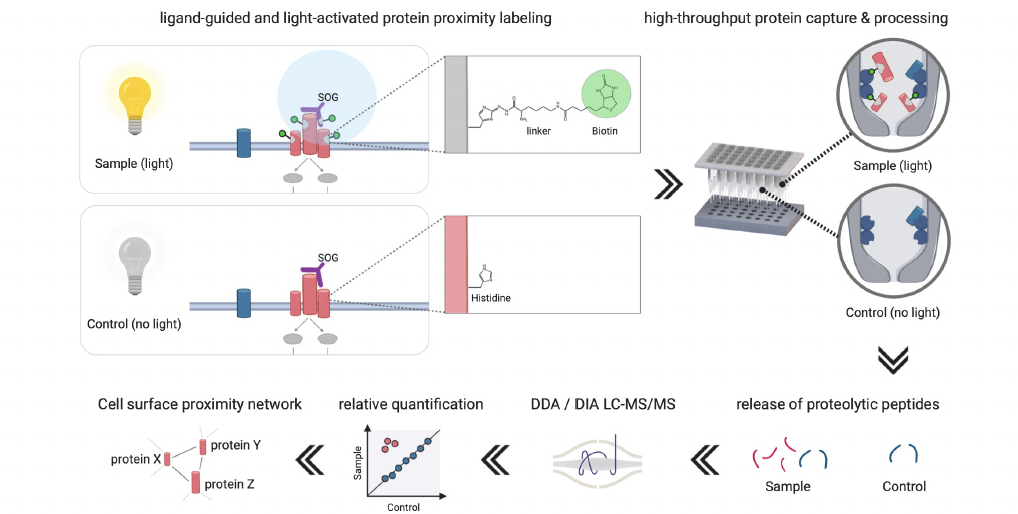
\includegraphics[width=1\textwidth]{Images/LUZ.png}\\[1cm]
\subsubsection{CD20 nanoscale organization on B-lymphoma cells}
Published CD20 interacting proteins
\begin{itemize}
    \item  MHC class I
(HLA-A!, HLA-A")
(FRET, Szöllosi et al. J. Immunol.)
\item MHCL class II
(HLA-DP!, HLA-DP")
(HLA-DQ!, HLA-DQ")
(HLA-DR!, HLA-DR")
(FRET, Szöllosi et al. J. Immunol.)
(Co-IP, Léveillé et al. Eur. J. Immunol.)
\item B-cell Receptor (CD79A, CD79B, IgM)
(Microscopy, Petrie et al. J. Immunol.)
(Co-IP, Polyak et al. J. Biol. Chem.)
(PLA, Kläsener et al. Elife)
\item  CD37 (suggested)
(FRET, Szöllosi et al. J. Immunol.)
\item CD40
(Co-IP, Léveillé et al. Eur. J. Immunol.)
\item CD71
(FRET, Szöllosi et al. J. Immunol.)
\item Tetraspanins (CD53, CD81, CD82) (weak)
\end{itemize}

\subsubsection{LUX-MS reveals antibody target and its acute surfaceome neighbourhood}
\begin{itemize}
    \item Deconvolution of antibody binding target
\item Lateral organization of CD20 on B-lymphoma cells
\item RTX-binding to CD20 affects B-cell receptor signaling 
\end{itemize}

\subsubsection{LUX labeling is restricted to target-expression cells and tunable by light}
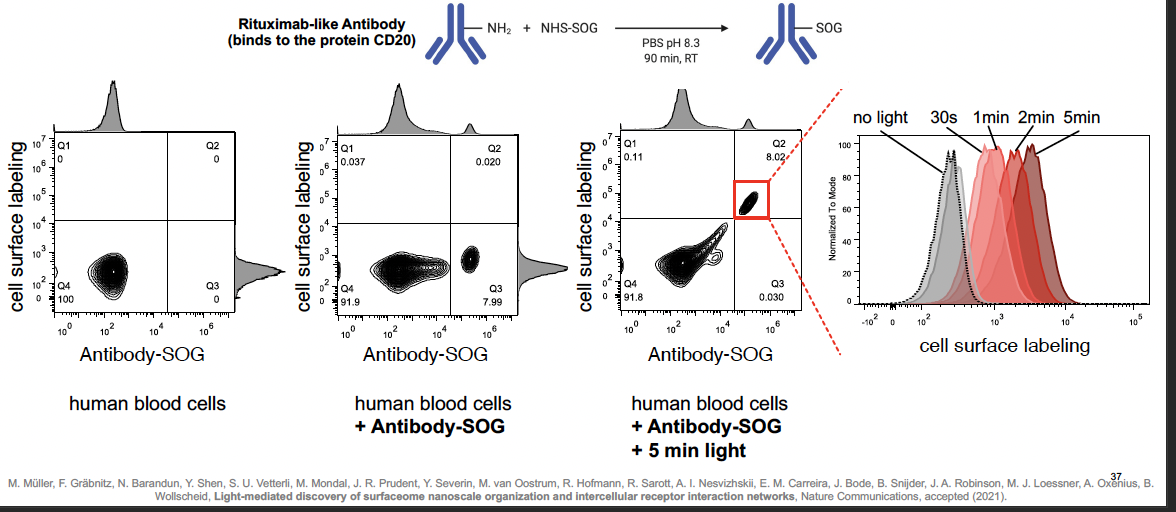
\includegraphics[width=1\textwidth]{Images/Labeling.png}\\[1cm]

\subsubsection{Establishing synchronized immune synapses around SOG coupled
antigens}
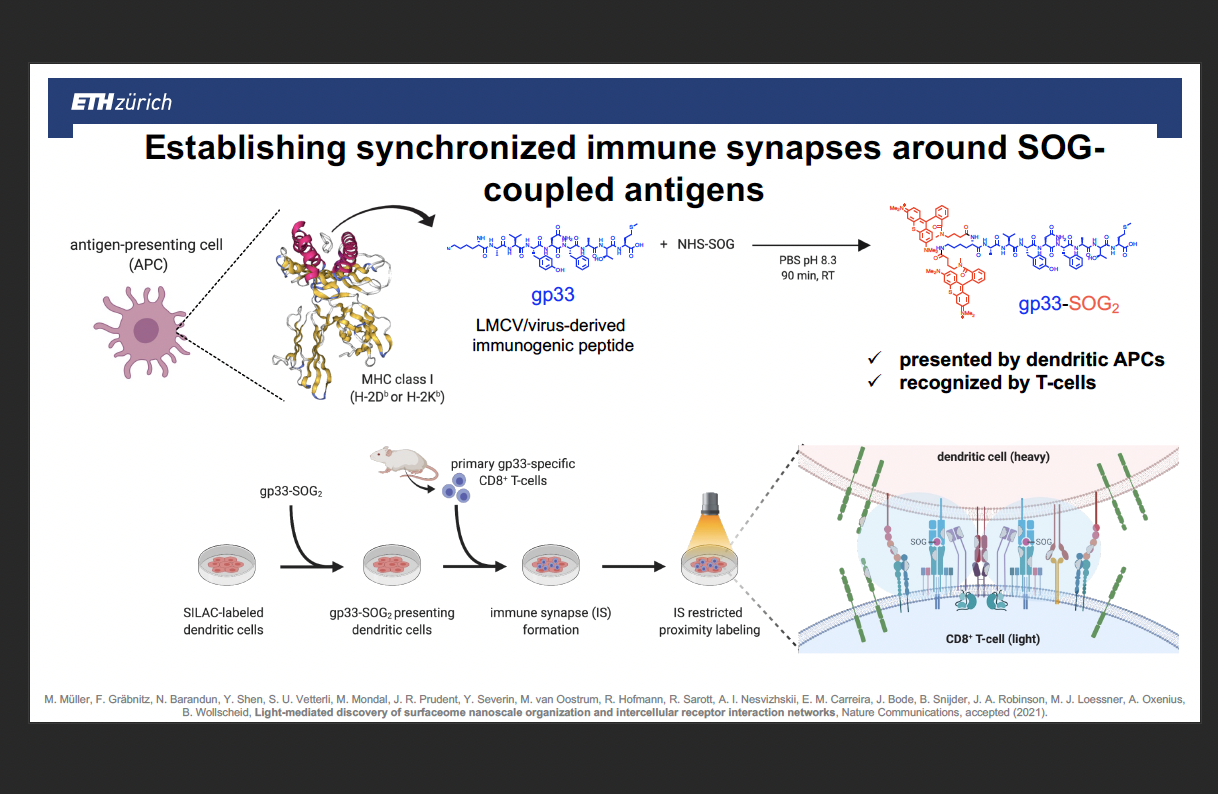
\includegraphics[width=1\textwidth]{Images/Synchro.png}\\[1cm]

\subsubsection{Elucidating intercellular signaling networks at the
Immunological Synapse}
\begin{itemize}
    \item LUX-derived proteotype model of the late-stage immune synapse:
\item Central downregulation of T-cell receptor (phagocytosis?)
\item IFNy-Receptor signaling at immunological synapse
\end{itemize}
\subsection{How can we utilize information about the surfaceome
architecture?}
\subsubsection{Utilizing surfaceome organization data to selectively kill
cancer cells}
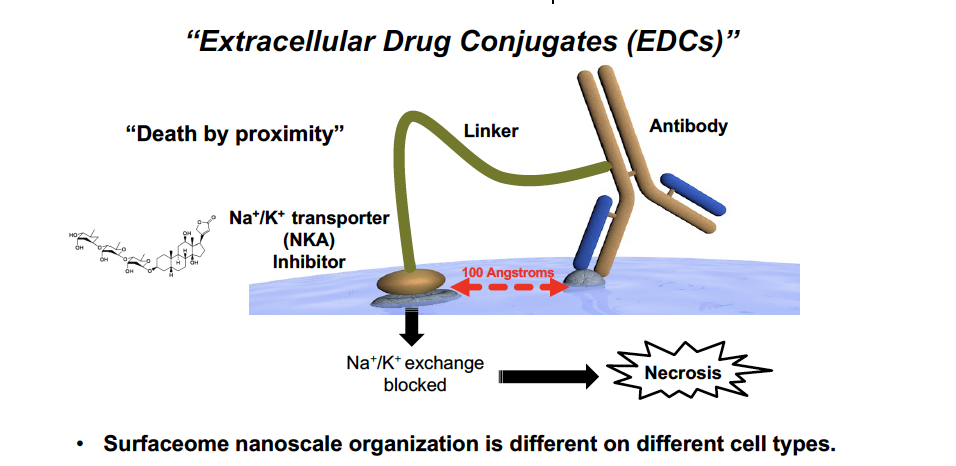
\includegraphics[width=1\textwidth]{Images/KillingCancer.png}\\[1cm]

\subsubsection{Colocalization-dependent targeting of cell sub-populations}
Study name: Designed protein logic to target cells with precise combinations of surfac antigens. BBy Marc Lajoie, Boyken (2020)
\\The Co-LOCKR strategy would enable the precise targeting of cell (sub-)populations based on detailed knowledge of the surfaceome architecture.

\subsubsection{Plug and Play for downstream application of therapeutic modalities}
See Beckmann (2021) for details

\subsubsection{Spatial proteotyping technologies aiding in the ra=onal
design of theranostic strategies to combat viral infections.}
This newly gained knowledge can in turn be leveraged now to combat viral infections using
innovative pharmaceutical strategies, targeting not only proteins residing within the drugaccessible
surfaceome, but rather host proteoform-centric complexes - as the mediators of
viral infection.

\subsubsection{Enabling the system-scale analysis of acute & dynamic
surfaceome interactions}
"Spatial Proteotyiping"
\\LUX-MS Technology enables detection of
acute & dynamic 
surfaceome interactions
\begin{itemize}
    \item  on a system-wide scale
\item in a light-controlled fashion
\item with ligands of any description
\item on living cells
\item across organisms
\item without the need for genetic manipulations
\end{itemize}

\section{Epigenetics}
\subsubsection{What is the Genome?}
A genome is the complete set of genetic information of an organism. It provides all the information an organism needs to function and it is shared among all cells of an organism.

\subsubsection{Is it the same among them all?}
In mammals, eurons are genetic mosaics due to retrotransposition early in development. Differences in the underlying genetic sequence could affect the epigenome of cells by modifying the binding of TFs and therefore the activity of regularory elements

\subsubsection{Epigenetics, what is it?}
All those regulated processes that, beginning with the genetic material, give rise to an organism.
As a field of researc, epigenetics emerged as an effort to understand unexpected observations.
\\Epigenetics is an umbrella term ; the study of molecular mechanisms that regulate gene transcription in eukaryotes


\subsubsection{Chromatin, what is it?}
Chromatin is a complex of proteins, RNA and DNA that constitutes the physiological state of the genome
\\It is the physiological template upon which transcriptional regulation occurs
\\essential for genome compaction within the nucleus
\\composition is highly dynamic during development and in response to environmental signals

\subsubsection{Eukaryotic Nucleus}
A eukaryotic nuncleus is a messy place. Thousands of regulatory decisions take place as we speak.
\\Gene regulation takes place in a context of adversity for the gene

\subsubsection{Epigenetic Mechanisms for the control of gene expression}
Different molecular mechanisms influence the transcriptional state of a gene
\\Nucleosomes: Make everything more compact
\\ATP-dependent chromatin remodelling complexes: Remodeller
\\CTCF and Cohesin: Architects
\\Histones and DNA: Modifiers
\\Histones and DNA: Readers I
\\DNA: Readers II

\subsubsection{REMEMBER}
while transcription factors (TFs) are not cosidered epigenetic regulators per se they are fundamental for epigenetic regulation as they recruit epigenetic modifiers to specific regions of the genome 


\subsection{The architecture of a gene
, what is it?}
\subsubsection{Regulatory elements modulate gene expression}
Regulatory elements are defined by biochemical signatures

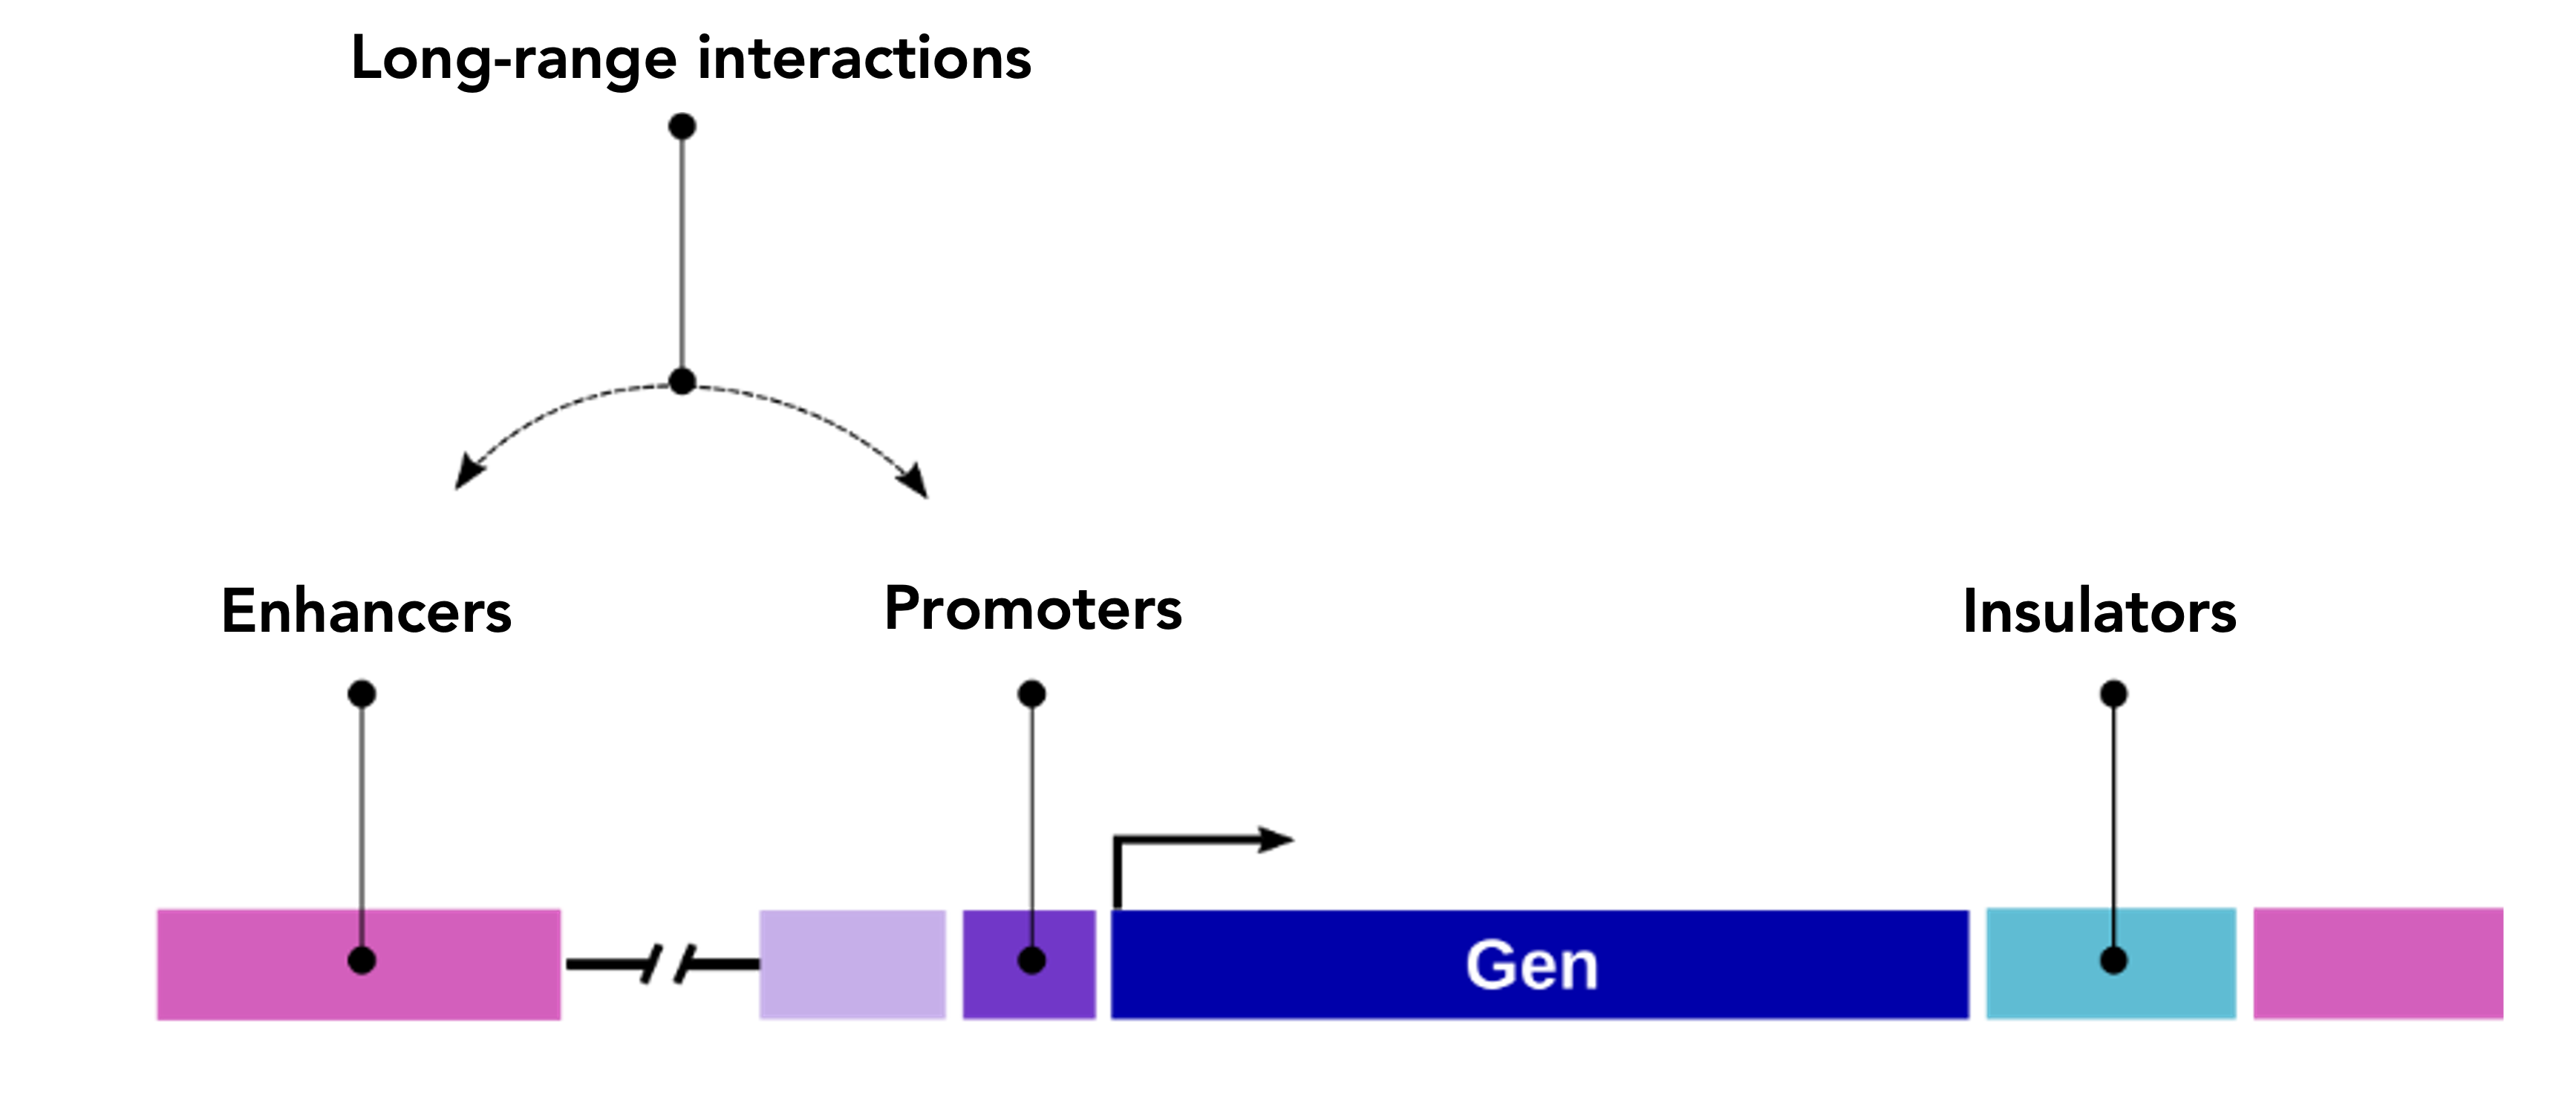
\includegraphics[width=1\textwidth]{Images/Epigenetics1.png}\\[1cm]

\subsection{Epigenome: What is it?}
The epigenome is the set of regulatory elements with biochemical signatures in a given cell type. The epigenome is made up of chemicals modifications and proteins that can associate  to the DNA and influence genome activity and integrity. Those biochemical modifications do not modify the DNA sequence but the change the way cells use the instructions encoded by regulatory elements

\subsection{What do we talk when we talk about Gene regulation?}
Regulatory Equilibrium
\\Regulatory genome, cell-type specific
\\DNA binding proteins, transcription factors
\\Epigenetic complexes, histone modifiers
\\Regulatory sequences, enhancers

\subsubsection{Epigenetic trait}
is a stably heritable phenotype resulting from changes in a chromosome without alterations in the DNA sequence.

\subsubsection{Brain function is strongly influenced by experience}
We are our experiences and the memory we have of them


\subsubsection{Emotional experiences can ave distinct physiological effects}
Can be distinguised frmo one another by their effect in the ability of the individual to cope with daily challenges

\subsubsection{Early life experiences can affect brain functions in adulthood 
}
Childhood is a sensitive period in life

\subsubsection{Childhood adversity alters cognitive and behavioral responses
}
Early life adversity is a significant risk factor for the development of mood disorders 
\\25$\%$ of the population experience cognitive and psychiatric disorders in adulthood  their etiology remains poorly understood 
\subsubsection{Remark}
Whether chromatin structure and its 3D organization 
are implicated in experience-dependent regulatory memory in brain cells remains controversial
\subsection{Chat GPT Based Full Epigenetics Notes}
Epigenetics is the study of heritable changes in gene function that do not involve changes to the underlying DNA sequence. These changes can include modifications to the DNA molecule itself or to the proteins with which DNA interacts. The term "epigenetics" was first coined by the British developmental biologist C. David Allis in the late 1990s to describe the study of how genetic information is passed from one generation to the next.

One of the key components of the epigenetic system is the nucleosome. A nucleosome is a unit of chromatin, which is the material that makes up chromosomes. Chromatin is composed of DNA and proteins, with the most abundant protein being histones. Histones are small, basic proteins that are rich in the amino acids lysine and arginine. They form a sort of "spool" around which DNA is wrapped, with about 147 base pairs of DNA wrapped around each histone octamer. Nucleosomes are formed by the winding of DNA around histones, and are the basic unit of chromatin organization.

Another important component of the epigenetic system is the ATP-dependent chromatin remodeling complex. These complexes are composed of proteins that can change the structure of chromatin by remodeling the nucleosomes. This can be done by sliding the histones along the DNA, by changing the position of the histones within the nucleosome, or by changing the overall shape of the nucleosome. Chromatin remodeling complexes are important for regulating gene expression, as they can change the accessibility of DNA to transcription factors, which are proteins that bind to DNA and control the rate at which genes are transcribed into RNA.

CTCF and cohesion are two other important components of the epigenetic system. CTCF is a protein that binds to DNA and regulates the organization of chromatin. It is involved in the formation of chromatin loops, which are regions of chromatin that are physically separated from each other but still interact with one another. Cohesion is the process by which sister chromatids, which are the identical copies of a chromosome that are formed during cell division, are held together. Cohesion is essential for the proper segregation of chromosomes during mitosis, the process by which a cell divides into two daughter cells.

DNA is the genetic material that contains the instructions for the development and function of all living organisms. It is made up of four nucleotide bases: adenine (A), thymine (T), cytosine (C), and guanine (G). These bases pair up in a specific way (A with T, and C with G) to form the "rungs" of the DNA ladder. The sequence of these bases determines the genetic code, which is read by the cell to make proteins, the building blocks of all living organisms.

Regulatory sequences are regions of DNA that control the rate at which genes are transcribed into RNA. These sequences can include enhancers, which are regions of DNA that increase the rate of transcription, and silencers, which are regions of DNA that decrease the rate of transcription. Enhancers and silencers can be located near a gene or far away from it, and can be activated or repressed by different signaling pathways.

Epigenetic complexes are groups of proteins that work together to control gene expression. These complexes can include DNA binding proteins, which bind to specific regions of DNA, and transcription factors, which bind to DNA and control the rate at which genes are transcribed into RNA. These complexes can also include histone modifying enzymes, which add or remove chemical groups to histones, changing their structure and function.

Chromatin is the material that makes up chromosomes. It is composed of DNA and proteins, with the most abundant protein being histones. Chromatin is organized into a hierarchical structure, with the most tightly packed form being heterochromatin, and the least tightly packed form being euchromatin. Heterochromatin is typically associated with regions of the genome that are not actively transcribed, while euchromatin is typically associated with regions of the genome that are actively transcribed. The organization of chromatin plays a crucial role in regulating gene expression, as it determines the accessibility of DNA to transcription factors and other regulatory proteins.

Epigenetic traits are heritable changes in gene function that do not involve changes to the underlying DNA sequence. These changes can include modifications to the DNA molecule itself or to the proteins with which DNA interacts. Epigenetic traits can be passed down from one generation to the next through the process of mitosis, the process by which a cell divides into two daughter cells. Epigenetic traits can also be influenced by environmental factors, such as diet, stress, and exposure to toxins.

Methylation and acetylation are two common epigenetic modifications that can occur on histones. Methylation is the process by which a methyl group is added to a histone, typically at lysine residues. This modification can lead to the formation of heterochromatin, which is associated with regions of the genome that are not actively transcribed. Acetylation is the process by which an acetyl group is added to a histone, typically at lysine residues. This modification can lead to the formation of euchromatin, which is associated with regions of the genome that are actively transcribed.

Methylation and acetylation take place at different stages of the cell cycle. Methylation typically occurs during interphase, when the cell is not actively dividing. Acetylation, on the other hand, typically occurs during the S-phase of the cell cycle, when DNA is replicated.

The step-by-step mechanism by which methylation occurs is as follows: 1) A methyltransferase enzyme binds to the histone, 2) S-Adenosyl-L-methionine (SAM) donates a methyl group to the histone, 3) The methyl group is added to the histone, typically at lysine residues. The consequences of methylation can lead to the formation of heterochromatin, which is associated with regions of the genome that are not actively transcribed.

The step-by-step mechanism by which acetylation occurs is as follows: 1) An acetyltransferase enzyme binds to the histone, 2) Acetyl-CoA donates an acetyl group to the histone, 3) The acetyl group is added to the histone, typically at lysine residues. The consequences of acetylation can lead to the formation of euchromatin, which is associated with regions of the genome that are actively transcribed.

In conclusion, epigenetics is a complex and dynamic field that involves the study of heritable changes in gene function that do not involve changes to the underlying DNA sequence. The epigenetic system is composed of various components, including nucleosomes, ATP-dependent chromatin remodeling complexes, CTCF and cohesion, histones, DNA, regulatory sequences, enhancers, epigenetic complexes, DNA binding proteins, transcription factors, chromatin, epigenetic traits, methylation, and acetylation. These components work together to control gene expression and influence the development and function of all living organisms. Understanding the mechanisms of epigenetics is essential for understanding the underlying causes of many human diseases, and for developing new therapies to treat these diseases.
\section{Clocks and Sleep: from Cells to Clinics}

\subsubsection{Why do we sleep?}
Because it's nighttime (circadian clock)
\\Because we're tired (sleep homeostasis)
\\A. Borbely's 2 process model is a model of sleep regulation that proposes that there are two distinct processes that govern sleep-wake behavior: the homeostatic process and the circadian process.

The homeostatic process, also known as the sleep drive, refers to the build-up of pressure for sleep as an individual stays awake. The longer an individual stays awake, the stronger the drive for sleep becomes. This process is thought to be regulated by a specific neurotransmitter, adenosine, which accumulates in the brain during wakefulness and is cleared during sleep.

The circadian process, on the other hand, refers to the 24-hour biological clock that regulates the timing of various physiological and behavioral processes, including sleep-wake cycles. This process is thought to be regulated by a specific set of cells in the hypothalamus called the suprachiasmatic nuclei (SCN), which respond to light signals and send signals to the rest of the body to regulate physiological processes.

The model suggests that these two processes interact with each other to regulate sleep-wake behavior. For example, the homeostatic process may push an individual to fall asleep, while the circadian process may keep them awake if it is not yet nighttime.

\subsection{Part I: Clocks}
\subsubsection{What are the Important Characteristics of a "Clock"?}
\begin{enumerate}
    \item It can be set to local time
\item It can tell you the time of day.
\item It can be used to measure lapse of time

\end{enumerate}

\subsubsection{Circadian Rhythms: The Basic Model}
Entrained circadian rhythms refer to the regular cycles of physiological and behavioral processes that align with the 24-hour light-dark cycle of the environment. These rhythms are regulated by the body's internal circadian clock and are synchronized with the external environment through cues such as light, temperature, and social cues. Entrained circadian rhythms are seen in many physiological processes, including the sleep-wake cycle, body temperature, and hormone levels.

\\Free-running circadian rhythms, on the other hand, refer to the natural, unaltered cycles of physiological and behavioral processes that occur in the absence of external cues. These rhythms are not influenced by the environment and are determined solely by the body's internal circadian clock. Free-running circadian rhythms can be observed in individuals living in isolation, such as in dark caves or in laboratory conditions where external cues are eliminated.

\\In summary, entrained rhythms are the rhythms that are synchronized with the environment, while free-running rhythms are the rhythms that are determined by the internal clock regardless of the environment.

\\We believe that light is taken up by photoreceptors, which give input to pacemakers, which give out a rhythm.


\subsubsection{To measure your inner clock}
\begin{enumerate}
    \item Take a skin biopsy
    \item Culture the cell
    \item Add a reporter-virus
    \begin{itemize}
        \item Human circadian gene + firefly light gene "luciferase"
    \end{itemize}
    \item Period length: the time for one cycle
    \item Amplitude: max vs min values
    \item Phase: when is the peak highest?
\end{enumerate}

\subsubsection{Detection}
In order to detect this phhenomenon, give the cells light with photomultiplier
\subsubsection{Chronotype correlates with cellular period length}

\subsubsection{Summary 1}
Larks are people whose biological clocks are “set
too early” or “run too fast”
\\Owls are people whose biological clocks are “set
too late” or “run too slow”
\\How is this medically relevant? We’ll find out soon.

\subsubsection{So, what is the mechanism of}
A genetic screen for defects in circadian rhytmicity leads to identification of the period locus in Drosophila

\subsubsection{and the same genes are important in mice}
Defect in clock genes leads to the loss of circadian behavior

\subsubsection{and in en and women}
Familial Advanced-Pase Sleep Syndrome (FASPS) is believed to be caused by a point mutation in te Per2 gene. 

\subsubsection{Basic design principle of circadian clocks: Negative feedback loop of transcription and translation}
The basic design principle of circadian clocks is the use of a negative feedback loop of transcription and translation. This refers to the process by which specific genes are activated (transcription) and the resulting protein products are produced (translation) in a cyclical manner, which then regulates the activity of the clock.

The negative feedback loop of transcription and translation is composed of two main components: the clock genes and the clock proteins. Clock genes are a group of genes that are responsible for encoding clock proteins, which are responsible for regulating the activity of the clock.

The negative feedback loop is initiated when clock genes are activated and the resulting clock proteins are produced. These clock proteins then interact with each other and inhibit the activity of the clock genes, thus closing the loop. This cycle of gene activation and protein production repeats itself in a 24-hour cycle, creating the circadian rhythm.

The negative feedback loop of transcription and translation is a fundamental mechanism that ensures the stability and precision of the circadian clock. The clock's ability to generate a self-sustaining rhythm, independent of the environment, but responsive to it makes it a robust, time-keeping mechanism.

\subsubsection{Model of the Mammalian Circadian Oscillator}
The model of the mammalian circadian oscillator is a theoretical framework that describes the molecular, cellular, and neural mechanisms that underlie the regulation of circadian rhythms in mammals.

The model is based on the discovery of a small group of genes known as clock genes, which are responsible for encoding clock proteins that regulate the activity of the circadian clock. These genes include CLOCK, BMAL1, PER, and CRY, which form a transcriptional-translational feedback loop.

The core of the model is a transcriptional-translational feedback loop that is composed of two main components: the positive element (CLOCK and BMAL1) and the negative element (PER and CRY). The positive element drives the transcription of the negative element, which in turn represses the activity of the positive element, thus closing the loop.

This feedback loop is responsible for the generation of a 24-hour rhythm in the expression of clock genes and clock proteins. The rhythmic expression of these genes and proteins is responsible for the regulation of various physiological and behavioral processes, including the sleep-wake cycle, body temperature, and hormone levels.

The model also includes the involvement of other signaling pathways, such as the MAPK pathway, which modulates the activity of the core loop. The model also includes the contribution of other brain regions such as the SCN (suprachiasmatic nuclei) which receives light signals and sends signals to the rest of the body to regulate the physiological processes.

In summary, the model of the mammalian circadian oscillator is a theoretical framework that describes the molecular, cellular, and neural mechanisms that underlie the regulation of circadian rhythms in mammals. It is based on the discovery of clock genes and the transcriptional-translational feedback loop that generates a 24-hour rhythm in the expression of clock genes and clock proteins.
\subsubsection{Circadian clocks control physiology}
\subsection{The circadian clock directly regulates the HPA axis}
Look at the slides for this

\subsubsection{Circadian glucocorticoids are just a part}
\subsubsection{The circadian clock controls metabolism}
he circadian clock plays a crucial role in controlling metabolism by regulating the timing of various metabolic processes throughout the day. Studies have shown that many metabolic pathways, including glucose metabolism, lipid metabolism, and energy expenditure, are under the control of the circadian clock.

The circadian clock controls glucose metabolism by regulating the timing of insulin secretion and glucose uptake in cells. Insulin secretion is highest during the daytime when glucose levels are typically high and lowest during the night when glucose levels are typically low. This ensures that glucose is used efficiently and stored when it is not needed.

The circadian clock also controls lipid metabolism by regulating the timing of fatty acid synthesis and breakdown. Fatty acid synthesis is highest during the daytime when energy levels are typically high and lowest during the night when energy levels are typically low. This ensures that fats are stored when they are not needed and used for energy when they are needed.

The circadian clock also controls energy expenditure by regulating the timing of thermogenesis, which is the production of heat by burning calories. Thermogenesis is highest during the daytime when energy levels are typically high and lowest during the night when energy levels are typically low. This ensures that energy is used efficiently and stored when it is not needed.

\subsubsection{Example: Glycogen storage and blood glucose}
\subsubsection{Clock dysfunction leads to metabolic syndrome}
Look at te slides

\subsubsection{People disturb their own clocks}

\subsubsection{Circadian clocks control mood and behavior}
Severe circadian disruption is associated with all depressive and affective disorders
\begin{itemize}
    \item Bipolar
    \item Depression
    \item Seasonal affective
    \item Schizophrenia
\end{itemize}

\subsubsection{All major neurotransmitter systems show defects in clock-deficient mice}

\subsubsection{Dopamine levels are elevated in Per2 mutant mice}
Dopamine is a neurotransmitter that is involved in a wide range of physiological and behavioral processes, including movement, motivation, and reward. Studies have shown that dopamine levels are elevated in Per2 mutant mice, which are mice that have a mutation in the Per2 gene, one of the core clock genes involved in regulating circadian rhythms.

Per2 is a gene that encodes the protein Period 2, which is an essential component of the transcriptional-translational feedback loop that generates circadian rhythms. In Per2 mutant mice, the gene is non-functional, leading to an alteration in the circadian rhythm of various physiological and behavioral processes.

Studies have shown that the alteration in the circadian rhythm of dopamine levels in Per2 mutant mice is caused by a disruption in the regulation of dopamine synthesis and release. Specifically, the mutation leads to an increase in the activity of the enzyme tyrosine hydroxylase (TH), which is responsible for the synthesis of dopamine. This results in an elevation of dopamine levels in the brain of Per2 mutant mice.

This elevation of dopamine levels in Per2 mutant mice has been associated with several behavioral changes, such as an increased activity level, hyperactivity, and impulsivity. These behavioral changes have been linked to changes in the activity of dopamine receptors and downstream signaling pathways, suggesting that the alteration in dopamine levels in Per2 mutant mice has a significant impact on brain function.
\subsubsection{Te clock regulates monoamine oxidase A and dopamine levels}
The circadian clock plays a role in regulating monoamine oxidase A (MAO-A) and dopamine levels. MAO-A is an enzyme that is responsible for the degradation of neurotransmitters such as dopamine. Studies have shown that the circadian clock regulates MAO-A expression and activity, which in turn affects dopamine levels.

During the day, when dopamine levels are typically high, MAO-A activity is low, allowing dopamine to remain at high levels in the brain. This is important for maintaining normal physiological and behavioral functions during the day. During the night, when dopamine levels are typically low, MAO-A activity increases, leading to the degradation of dopamine and ensuring that dopamine levels are low at night.

Studies have also shown that the circadian clock also regulates the expression of dopamine receptors and downstream signaling pathways, which in turn affects dopamine levels. For example, dopamine receptors are typically more active during the day when dopamine levels are high and less active at night when dopamine levels are low.

Disruptions in the circadian clock, such as those caused by mutations in clock genes or disruptions in the light-dark cycle, can lead to changes in the levels of dopamine and MAO-A. This can result in changes in behavior, mood, and other physiological functions.
\subsubsection{The circadian clock controls memory}
Hippocampal-dependent learning requires a functional circadian system

\subsubsection{Rest-activity consolidation favors organisation of synaptic potentiation and downscaling}
Rest-activity consolidation refers to the process by which the brain consolidates information and memories during periods of rest or sleep. It is believed that this process is necessary for organizing and strengthening neural connections, which is essential for learning and memory.

During periods of rest or sleep, the brain is thought to be in a state of synaptic potentiation, which refers to the strengthening of neural connections. This is thought to be necessary for the consolidation of new information and memories.

On the other hand, during periods of activity or wakefulness, the brain is thought to be in a state of synaptic downscaling, which refers to the weakening or elimination of neural connections that are no longer needed. This is thought to be necessary for the elimination of irrelevant information and memories.

The process of rest-activity consolidation is thought to be facilitated by the release of specific neurotransmitters and neuromodulators, such as dopamine, acetylcholine, and GABA, which are involved in the regulation of synaptic plasticity.

Studies have shown that rest-activity consolidation is affected by disruptions in the circadian clock, such as those caused by mutations in clock genes or disruptions in the light-dark cycle. These disruptions can lead to changes in the timing of synaptic potentiation and downscaling, which can affect learning and memory.


\subsubsection{Disrupting clock control of synaptic function leads to intellectual disability}
Mutations in NONO lead to syndromic intellectual disability and inhibitory synaptic defects

\subsubsection{Summary 2}
\begin{itemize}
    \item Feedback loops of transcription and
translation regulate circadian clocks
\item Distinct molecular mechanisms control
circadian metabolism, mood, and memory

\end{itemize}
Disruption of these clocks results in diverse
physiological morbidities 

\subsection{Part II: Sleep}
\subsubsection{How do we recognize sleep?}
\subsubsection{A few universal ideas about sleep/rest}
\begin{enumerate}
    \item Distinct posture
\item Reduced environmental awareness
\item Homeostatic regulation: "the less you get, the more you want"
\end{enumerate}

\subsubsection{But come on, does a fly really sleep?
}
The same drugs that affect your sleep, affect their
“sleep”.
\begin{itemize}
    \item  Caffeine
\item Benzodiazepines
\item Many more
\end{itemize}
Genetic mutations in shared genes that affect your
sleep, affect their “sleep”.

\subsubsection{We define sleep stages by the kinds of EEGG waves seen at each stage}
Awake, NREM, and REM.

\subsubsection{EEG waves reflect underlying neuronal synchrony}

\subsubsection{We go through several cycles of sleep each night}
\subsubsection{Sleep oscillations (especially slow waves) increase with greater sleep pressure}

\subsubsection{How are sleep oscillations regulated?}
Sleep oscillations are regulated by the interaction of different neural systems in the brain, including the "flip-flop switch" mechanism. The flip-flop switch refers to the alternating activity of two groups of neurons in the hypothalamus, the ventrolateral preoptic nucleus (VLPO) and the tuberomammillary nucleus (TMN), during different stages of sleep. The VLPO is active during non-REM sleep and promotes sleep by inhibiting the activity of wake-promoting neurons in the TMN. The TMN is active during REM sleep and promotes wakefulness by inhibiting the activity of sleep-promoting neurons in the VLPO. This flip-flopping activity between these groups of neurons helps to regulate the alternation between non-REM and REM sleep, and between wakefulness and sleep.
\subsubsection{Sleep-wake models}
There are several different models that have been proposed to explain the regulation of sleep and wakefulness in the brain. Some of the main ones include:

\\The two-process model of sleep regulation: This model proposes that there are two main processes that regulate sleep and wakefulness: a homeostatic process that builds up during wakefulness and is released during sleep, and a circadian process that is driven by an internal biological clock.
\\The reciprocal interaction model: This model proposes that there are two groups of neurons in the brain that promote wakefulness and sleep, respectively, and that they are in a state of reciprocal inhibition.
\\The ascending arousal model: This model proposes that there is a system of ascending arousal in the brainstem that promotes wakefulness, and that this system is modulated by several other neural systems, such as the circadian rhythm and the homeostatic process.
The flip-flop model: This model proposes that there are two groups of neurons in the hypothalamus that promote wakefulness and sleep respectively, and they are in a state of reciprocal inhibition.
\\The sleep-wake homeostasis model: It suggest that there's a process that builds up during wakefulness and is released during sleep and the accumulation of this process during wakefulness will increase the drive for sleep.
It's worth noting that these models are not mutually exclusive, but rather complementary and provide different perspectives on the regulation of sleep and wakefulness.

\\The CT-TC loops model: This model proposes that there are two types of neural circuits in the brain that promote wakefulness and sleep, respectively: the cholinergic-thalamo-cortical (CT) loop and the GABAergic-thalamo-cortical (TC) loop. The CT loop is active during wakefulness and promotes arousal, attention and cognition. The TC loop is active during sleep and promotes inhibition and unconsciousness. This model suggests that the balance between the activity of these two loops regulates the transitions between wakefulness and sleep.
\\The GABA-glutamate model: This model proposes that the balance between the activity of the neurotransmitters GABA and glutamate in the brain plays a key role in regulating sleep and wakefulness. GABA is an inhibitory neurotransmitter that promotes sleep and reduces arousal, while glutamate is an excitatory neurotransmitter that promotes wakefulness and increases arousal. This model suggests that the balance between the activity of these two neurotransmitters regulates the transitions between wakefulness and sleep.
\subsubsection{Narcolepsy}
The loss of wake-promoting hypothalamic neurons results in REM sleep during excitement

\subsubsection{How are sleep and sleep EEG waves useful?}
The state of sleep facilitates cellular rebuilding processes
\\Metabolism: Real time breath analysis across a night of sleep. 2016 differentially expressed features detected 4320 metabolomes/night
\\Nearly all metabolism is orchestrated across sleep state
\\Sleep favors global synaptic downscaling
\\Sleep waves synchronize the transfer of memories from one brain location to another. At the simplest level, this is what dreams are: movement and strengthening memories. Potential mindmap:
\begin{enumerate}
    \item Hippocampo-neocortical communication
    \item Selective refining of memory representations/rescaling of synaptic weight
    \item Strengthening of neocortical memory  representations
\end{enumerate}

\subsubsection{Place cells: neurons that fire (mostly) when you are at a certain place}
Look at Aterton TINS 2015 study

\subsubsection{Summary 3}
Sleep oscillations are controlled globally and locally
\\Sleep oscillations control metabolism and cognitive function